% AThesis v2.2

% این قالب بر اساس فرمت پایان‌نامه‌ها و رساله‌های تحصیلات تکمیلی دانشگاه صنعتی اصفهان تهیه شده است.

% ارسال نظرات جهت بهبود قالب:
% a101.fakhari@gmail.com

% توصیه می‌شود که از توزیع تک‌لایو (TexLive) استفاده شود:
% http://tug.org/texlive/acquire-iso.html

% از نصب بودن فونت B ZAR و B Zar Bold بر روی سیستم خود اطمینان حاصل کنید. اگر به مشکل پیدا نکردن فونت برخوردید، از وجود این فونت ها در پوشه Windows/Fonts از طریق CMD مطمین شوید.
% کمپایلر ادیتور را روی XeLaTeX قرار دهید.

% موفق باشید.
% امین فخاری
% ‌دی‌ماه 1394
% -----------------------------------------------------------------------------------

% نکات:

% برای آن‌که پردازش فایل و مشاهده خروجی در هنگام نوشتن پایان‌نامه آسان‌تر و سریع‌تر انجام شود، انجام موارد زیر توصیه می گردد:
% الف) فصل‌ها و بخش‌هایی که در حال نوشتن آن‌ها نیستید را غیر فعال کنید. به‌عنوان مثال، در این قالب، این دستورات را می‌توان در صورت عدم نیاز با اضافه کردن % به طور موقت غیرفعال کرد:
% \MakeTitlePage
% \MakeFarsiSignaturePage
% \input{Chapters/nowledgments}
% \MakeCopyRightPage
% \clearpage
\thispagestyle{empty}
\newgeometry{left=3cm,right=4cm,top=7cm}

{\BZarScaleOne
{\fontsize{28pt}{0}\selectfont
\noindent
% تقدیم اثر---------------------------------------------------------
تقـدیم به
\\[1cm]
\hspace*{1cm}
مادرم به مهربانی فرشته
% ؛---------------------------------------------------------
}}
		
\restoregeometry
% \MakeTableOfContents
% \MakeListOfFigures
% \MakeListOfTables
% \MakeFarsiAbstract
% \input{Chapters/Chapter#}
% \MakeAppendices
% \section{جزئیات اشتباهات مدل}
\setlength{\hoffset}{0cm}
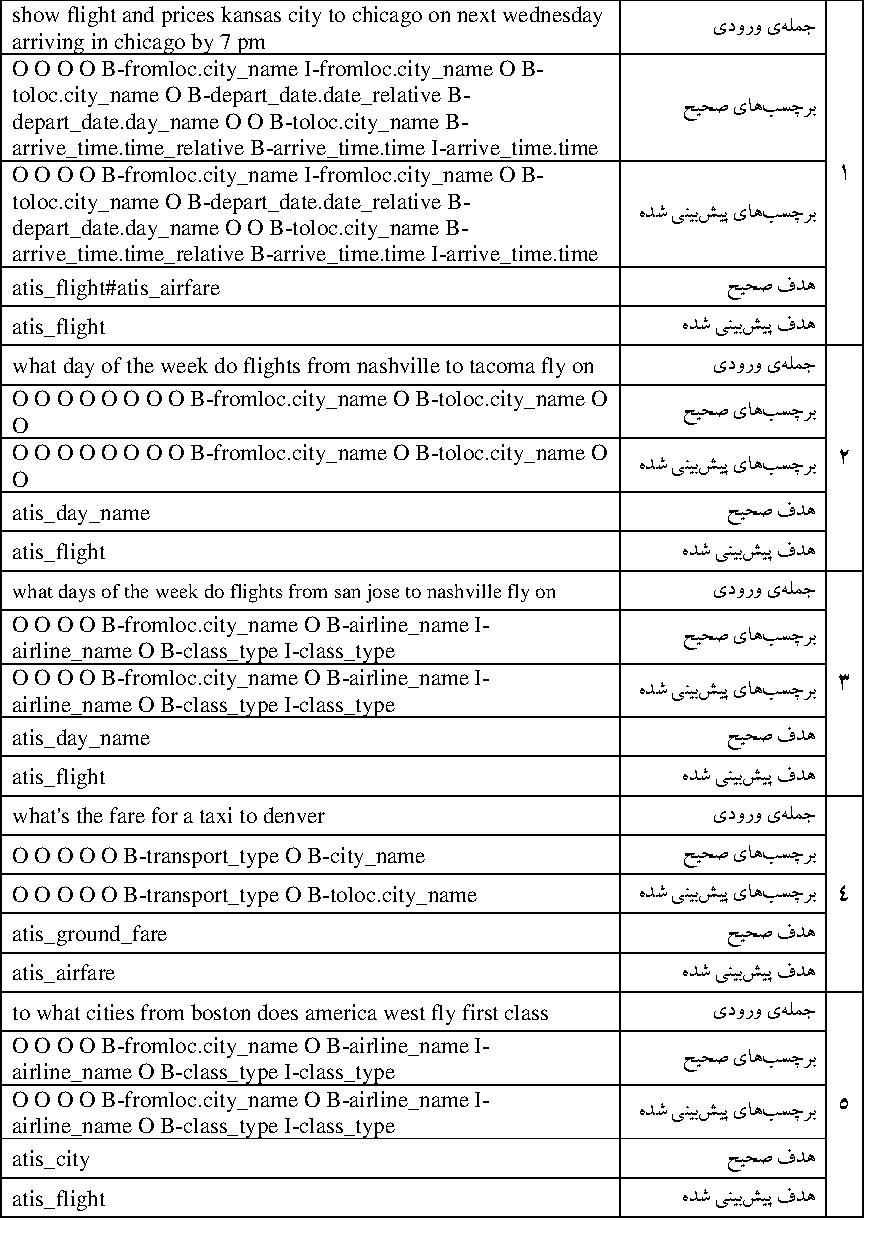
\includepdf[pages=1,nup=1x1,pagecommand={\rl{\subsection{اشتباهات در مجموعه داده‌ی\lr{ATIS}}}}\vspace{-\baselineskip},width=(\textwidth*8/9)]{Tables/atiserrors.pdf}
\includepdf[pages=2-,nup=1x1,pagecommand={},width=(\textwidth*1)]{Tables/atiserrors.pdf}
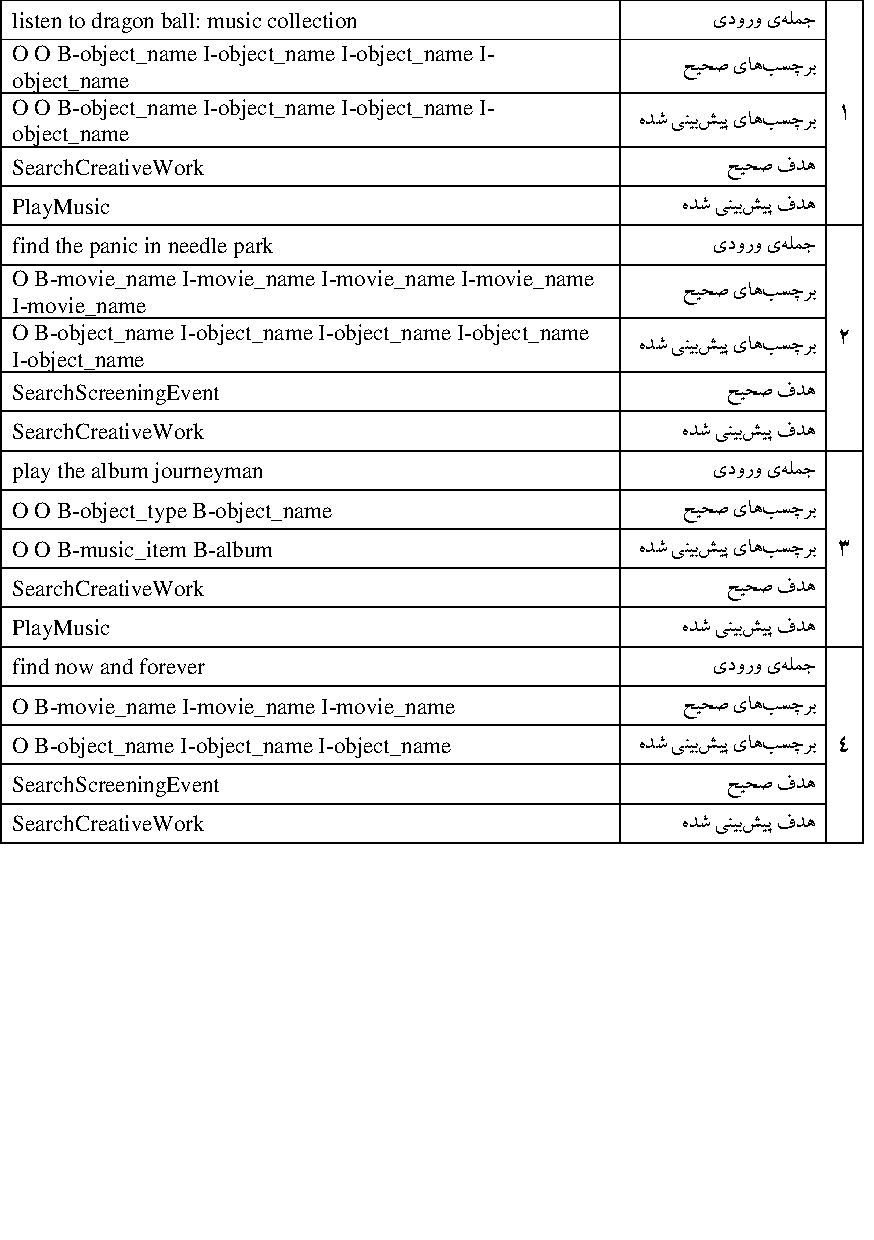
\includepdf[pages=1,nup=1x1,pagecommand={\rl{\subsection{اشتباهات در مجموعه داده‌ی\lr{SNIPS}}}}\vspace{-\baselineskip},width=(\textwidth*8/9)]{Tables/snipserrors.pdf}
%\includepdf[pages=2-,nup=1x1,pagecommand={},width=(\textwidth*1)]{Tables/snipserrors.pdf}

% \MakeEnglishAbstract
% \MakeEnglishSignaturePage
% ب) از گزینه draft برای فراخوانی کلاس استفاده کنید. یعنی
% \documentclass[a4paper,fleqn,10pt,oneside,draft]{book}
% این گزینه حالت چرکنویس را ایفا می‌کند و بر روی بسته‌های مختلف اثرهای متفاوتی دارد. به‌عنوان مثال: به جای شکل، تنها چهارچوب آن نمایش داده شود، لینک‌های hyperref غیر فعال گردد، فایل‌های خارجی را در بسته listings اضافه نمی‌کند و ... و همه این موارد سبب کاهش زمان اجرا و حجم فایل می‌شود.

% در صورتی که میخواهید به سطر بعد بروید اما نمیخواهید بین دو کلمه‌ای که نوشتید فاصله بیفتد کافی است در انتهای خط اول  (بدون فاصله) کاراکتر % را اضافه کنید. با این عمل، لاتک خط فاصله ایجاد شده در اثر تغییر سطر را به عنوان توضیح اضافه یا کامنت در نظر میگیرد و در خروجی اعمال نمی‌کند.

% توصیه می‌شود از شکل‌های برداری با فرمت PDF استفاده شود. این کار علاوه بر افزایش کیفیت رسال/پایان‌نامه/گزارش، باعث کاهش حجم شکل‌ها (و در نتیجه  کاهش حجم فایل نهایی) و همچنین کاهش زمان پردازش می‌شود.

% در این قالب سعی شده است که از تمامی بخش‌های موجود در پایان‌نامه‌ها نمونه‌ای آورده شود.

\documentclass[a4paper,fleqn,10pt,oneside]{book}
%-----------------------------
% بسته‌های دلخواه را در این قسمت اضافه نمایید:
\usepackage{colortbl} % برای تنظیم رنگ خط جدول
\usepackage{longtable} % برای جدول های طولانی
\usepackage{ragged2e} % برای جاستیفای کردن انگلیسی ابسترکت
\usepackage{setspace} % برای تنظیم اندازه خط ها در ابسترکت
\usepackage{pifont} % برای بولت ها
\usepackage[hyphens]{url}
\usepackage{hyperref}
%-----------------------------
\usepackage[final]{pdfpages}
\usepackage{Settings/AThesisStyle}

%-----------------------------
% دستورهای مورد نیاز را در این قسمت اضافه نمایید:

%-----------------------------

\begin{document}

\pagestyle{plain}
\pagenumbering{adadi}
\setcounter{page}{2}

% ░░░░░░░▒▒▒▒▒▒▓▓▓▓ In the Name of Allah ▓▓▓▓▒▒▒▒▒▒░░░░░░░
%%\clearpage
%%\thispagestyle{empty}
%%\begin{figure}[t]
%%\centering
%%
\includegraphics[scale=1.3]{Settings/Allah.pdf}
%%\end{figure}

% ░░░░░░░▒▒▒▒▒▒▓▓▓▓ Title Page ▓▓▓▓▒▒▒▒▒▒░░░░░░░
\DepartmentFa{دانشکده مهندسی برق و کامپیوتر}
%%\ThesisTypeFa{رساله} % 
\ThesisTypeFa{پایان‌نامه}% Or \ThesisTypeFa{پیشنهادیه پایان‌نامه}
%%\DegreeFa{دکتری} % Or 
\DegreeFa{کارشناسی ارشد}
\FieldFa{مهندسی نرم‌افزار}
\YourFullnameFa{مهرداد رفیعی‌پور}
\FirstSupervisorFa{دکتر جواد سلیمی سرتختی}
\FirstAdvisorFa{دکتر فرشته دهقانی}
%\SecondSupervisorFa{دکتر فرشته دهقانی} % Optional (Remove It If You Don't Have)
\YearFa{1401}
\TitleFa{
ارائه‌ی یک مدل برای درک زبان طبیعی
\\[0.4cm]
%%توسط انگشتان نرم
 با استفاده از شبکه‌های عصبی عمیق
}
% اگر عنوان رساله طولانی بود، در دو خط به صورت نشان داده شده تقسیم شود.

\MakeTitlePage

% ░░░░░░░▒▒▒▒▒▒▓▓▓▓ Signature - Farsi ▓▓▓▓▒▒▒▒▒▒░░░░░░░
\Prefix{آقای} %\Prefix{خانم}
\DateFa{1401/11/30}
\FirstAdvisorFa{دکتر فرشته دهقانی}
%\SecondAdvisorFa{دکتر مشاور دوم} % Optional (Remove It If You Don't Have)
\FirstExaminerFa{}
\SecondExaminerFa{} % Optional (Remove It If You Don't Have)
\ThirdExaminerFa{} % Optional (Remove It If You Don't Have)
%\FourthExaminerFa{دکتر داور چهارم} % Optional (Remove It If You Don't Have)
%\FifthExaminerFa{دکتر داور پنجم} % Optional (Remove It If You Don't Have)
\DeanOfDepartmentFa{}

%\MakeFarsiSignaturePage

% ░░░░░░░▒▒▒▒▒▒▓▓▓▓ Acknowledgments ▓▓▓▓▒▒▒▒▒▒░░░░░░░
%%\clearpage
\thispagestyle{empty}
\newgeometry{left=3cm,right=4cm,top=7cm}

{\BZarScaleOne
{\fontsize{20pt}{0}\selectfont
\noindent
% عنوان تشکر و قدردانی---------------------------------------------------------
تشکر و قدردانی
% ؛---------------------------------------------------------
}}
\vspace{0.5cm}

{\BZarScaleOne
{\fontsize{12pt}{0.9cm}\selectfont % Zar 13
\noindent
% متن تشکر و قدردانی---------------------------------------------------------
جناب دکتر سلیمی استاد راهنمای محترم\\
سرکار خانم دکتر دهقانی استاد مشاور گرانقدر






% ؛---------------------------------------------------------
}}

\restoregeometry

% ░░░░░░░▒▒▒▒▒▒▓▓▓▓ CopyRight ▓▓▓▓▒▒▒▒▒▒░░░░░░░
%%\MakeCopyRightPage

% ░░░░░░░▒▒▒▒▒▒▓▓▓▓ Dedication ▓▓▓▓▒▒▒▒▒▒░░░░░░░
\clearpage
\thispagestyle{empty}
\newgeometry{left=3cm,right=4cm,top=7cm}

{\BZarScaleOne
{\fontsize{28pt}{0}\selectfont
\noindent
% تقدیم اثر---------------------------------------------------------
تقـدیم به
\\[1cm]
\hspace*{1cm}
مادرم به مهربانی فرشته
% ؛---------------------------------------------------------
}}
		
\restoregeometry

% ░░░░░░░▒▒▒▒▒▒▓▓▓▓ Abstract - Farsi ▓▓▓▓▒▒▒▒▒▒░░░░░░░
\AbstractFa{
با افزایش محبوبیت تلفن‌های هوشمند، استفاده از ابزارهای مبتنی بر سیستم گفت‌وگو نیز به طرز چشم‌گیری افزایش داشته است. درک زبان طبیعی، بخشی حیاتی از یک سیستم گفت‌وگو است؛ چراکه نقص در آن باعث ایجاد گلوگاه در چرخه‌ی عملکرد سیستم گفت‌وگو می‌شود. تشخیص هدف کاربر و پرکردن جای خالی، دو وظیفه‌ی اصلی درک زبان طبیعی هستند. 
شبکه‌های عصبی بازگشتی به طور گسترده برای بهبود این وظایف مورد بررسی قرار گرفته‌اند، اما دارای ضعف‌های شناخته شده‌ای مانند گرادیان محو شونده و زمان آموزش بالا هستند. به تازگی، ترنسفورمر برای رفع ایرادات مذکور معرفی شده است. از طرف دیگر، تعداد کمی از کارهای پیشین، خروجی مدل‌های زبانی را برای کار مورد نظر تعبیه می‌کنند.
در این پایان‌نامه، مدل \lr{CTran} معرفی می‌شود. \lr{CTran} یک مدل رمزنگار-رمزگشا‌ی مبتنی بر شبکه‌ی عصبی کانولوشنی و ترنسفورمر است که برای دو چالش تشخیص هدف و پرکردن جای خالی طراحی شده است. در رمزنگار \lr{CTran}، از بِرت به عنوان فراهم کننده‌ی تعبیه‌ی اولیه واژه ها استفاده شده است. سپس، یک لایه‌ی کانولوشنی با اندازه‌های هسته‌ی متفاوت استفاده شده، خروجی آن ترانهاده و سپس الحاق شده است. در بخش آخر رمزنگار، خروجی به یک پشته‌ی رمزنگار ترنسفورمر تغذیه شده تا تعبیه‌ی جمله‌ی ورودی تکمیل شود. در \lr{CTran} به منظور تولید خروجی برای هر وظیفه، دو رمزگشای جداگانه معرفی شده، که هردو یک رمزنگار را به طور مشترک استفاده می‌کنند. برای رمزگشای تشخیص هدف، مکانیزم توجه به خود و به دنبال آن از یک لایه‌ی خطی تماماً متصل به کار گرفته شده است. برای رمزگشای پرکردن جای خالی، رمزگشای ترنسفورمر تراز شده معرفی گردیده است. برای تراز کردن رمزگشای ترنسفورمر، از ماتریس قطری استفاده شده است. ماتریس قطری، موقعیت‌های متناظر با برچسب‌های هدف در رمزنگار را، در دسترس قرار داده و سایر موقعیت‌ها را مخفی می‌کند. در انتهای کار، به منظور سنجش صحت عملکرد مدل پیشنهادی، مدل بر روی دو مجموعه داده‌ی \lr{ATIS} و \lr{SNIPS} آزمایش گردید. نتایج آزمایش‌ها نشان می‌دهد که مدل پیشنهادی در تشخیص جای خالی، بر روی هر دو مجموعه داده، عملکرد بهتری از مدل‌های پیشین دارد. علاوه بر این، عملکرد دو استراتژی مدل زبانی به عنوان رمزنگار و مدل زبانی به عنوان تعبیه واژه‌ها، سنجیده شد. نتایج نشان می‌دهد که استراتژی استفاده از مدل زبانی تنها به عنوان تعبیه‌ی واژه‌ها، عملکرد بهتری دارد.
}

\KeywordsFa{
1-شبکه‌ی عصبی عمیق،  2-پردازش زبان طبیعی، 3-درک زبان طبیعی،  4-تشخیص هدف در متن، 5-پر کردن جای خالی در متن
}
\MakeFarsiAbstract

% ░░░░░░░▒▒▒▒▒▒▓▓▓▓ Table of Contents/Figures/Tables ▓▓▓▓▒▒▒▒▒▒░░░░░░░
\MakeTableOfContents
\MakeListOfFigures
\MakeListOfTables

% ----------------------------------------------------------------------------
\clearpage
\pagestyle{myheadings}
\pagenumbering{arabic}
\setcounter{page}{1}

% ░░░░░░░▒▒▒▒▒▒▓▓▓▓ Chapters ▓▓▓▓▒▒▒▒▒▒░░░░░░░
\clearpage
\baselineskip=0.9cm

\chapter{پیش‌درآمد}
\pagebreak
\section{مقدمه}
در فصل پیش رو، مقدمه‌ای بر مسئله‌ی درک زبان طبیعی بیان می‌شود. در ادامه، از کاربرد آن در سیستم‌های گوناگون و سیستم‌های امروزی سخن گفته شده و اهمیت آن تبیین گردیده است. در این راستا،  ابتدا تعریف مسئله‌ی درک زبان طبیعی و دو وظیفه‌ای که پایه‌های مسئله را تشکیل داده‌اند گفته شده است و در ادامه، اهمیت مسئله و کاربرد آن را در دنیای واقعی تشریح شده است.
\section{تعریف مسئله: طراحی یک مدل برای درک زبان طبیعی}
سیستم گفت‌وگو\LTRfootnote{Dialogue System}
 یک برنامه‌ی رایانه‌ای است که برای تعامل با انسان از طریق متن یا صوت طراحی شده است. سیستم گفت‌وگو از طریق شبیه‌سازی مکالمه با انسان، امکان خودکارسازی امور را افزایش می‌دهد. در نتیجه، استفاده از آن باعث سادگی تعامل انسان با رایانه و افزایش دسترسی به اطلاعات و امکانات سیستم رایانه‌ای می‌شود.
در یک سیستم گفت‌وگو، کاربر سؤالی را به زبان طبیعی مطرح می‌کند که پاسخ آن درون پایگاه دانش قرار دارد. وظیفه‌ی سیستم گفت‌وگو این است که هدف و اطلاعات مهم معنایی را از سؤال استخراج کرده و ضمن پیدا کردن پاسخ مناسب از پایگاه دانش، جوابی فراخور را به کاربر نمایش دهد. بدین منظور، مطابق شکل \ref{Fig:dialoguesystem}، در ابتدا سوال کاربر وارد واحد درک زبان طبیعی\LTRfootnote{Natural Language Understanding} می‌شود. این واحد هدف و ترکیبات معنایی موجود در سوال را استخراج کرده و در اختیار واحد مدیریت مکالمه\LTRfootnote{Dialogue Management Unit} قرار می‌دهد. واحد مدیریت مکالمه، وظیفه‌ی نگهداری و ردیابی مکالمه‌ی کاربر و همچنین تعامل با پایگاه دانش را برعهده دارد.  این واحد با توجه به سیاست‌‌های\LTRfootnote{Policy} موجود، تصمیمی را اتخاذ کرده و آن را در اختیار واحد تولید زبان\LTRfootnote{Language Generation Unit} قرار می‌دهد، تا این واحد اقدام به تولید پاسخ کند. توانایی کاربر به سؤال کردن محدود نمی‌شود؛ بلکه می‌تواند درخواست انجام عمل نیز بدهد. در این صورت، به جای تولید پاسخ به زبان طبیعی، عمل مناسب توسط سیاست‌های موجود در پایگاه دانش مشخص شده و به واحد مدیریت مکالمه ابلاغ می‌شود.
\begin{figure}[!htb]
	\centering
	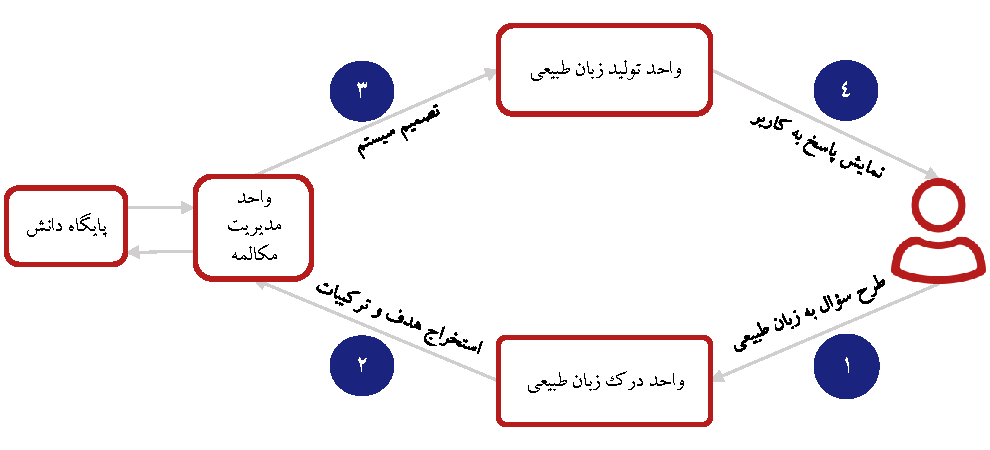
\includegraphics[scale=0.9]{Figures/dialoguesystem.pdf}
	\caption{فرایند عملکرد سیستم‌های گفت‌وگو}
	\label{Fig:dialoguesystem}
\end{figure} 


همانطور که در شکل \ref{Fig:dialoguesystem} مشهود است، درک زبان طبیعی نخستین بخش در چرخه‌ی عملکرد سیستم گفت‌وگو است. این امر بیانگر نقش حیاتی این سیستم است؛ به نحوی که نقص در عملکرد این بخش منجر به ایجاد گلوگاه\LTRfootnote{Bottleneck} برای سایر اجزاء سیستم می‌شود.
 درک زبان طبیعی شامل دو وظیفه‌ی "تشخیص هدف"\LTRfootnote{Intent-Detection} و "پرکردن جای خالی"\LTRfootnote{Slot-Filling} است.  غایت در وظیفه‌ی تشخیص هدف، پیش‌بینی منظور کاربر از سوال مطرح شده است. همچنین، پرکردن جای خالی به معنای استخراج اطلاعات معنایی\LTRfootnote{Semantic Information} از درون جمله است. اطلاعات معنایی، واژه‌هایی از جمله هستند که دارای نام، کد، زمان و اطلاعاتی بوده که به تکمیل وظیفه کمک می‌کنند. پر کردن جای خالی را می‌توان به عنوان یک مسئله‌ی برچسب‌زنی توالی\LTRfootnote{Sequence Labeling}، و تشخیص هدف را به عنوان یک مسئله‌ی کلاس‌بندی\LTRfootnote{Classification} تعریف کرد.
 
 
برای تعریف رسمی مسئله، تعداد واژه‌ها در زبان کاربر با $V$، تعداد برچسب‌های یکتا با $T$، تعداد اهداف یکتا در مجموعه داده با $I$ و تعداد واژه‌های سؤال با $n$، نمایش داده می‌شود. در این صورت، کاربر سوال خود را در قالب $Q=\{q_{1},q_{2},q_{3},\cdots,q_{n}\} , q_{i}\in\mathbb{W}^{V}$ مطرح می‌کند. واحد درک زبان طبیعی به ازاء هر $Q$، یک هدف $i\in\mathbb{W}^{I}$، و ترتیب $S$ که به صورت $S=\{s_{1},s_{2},s_{3},\cdots,s_{n}\} , s_{i}\in\mathbb{W}^{T}$ تعریف می‌شود را، تولید خواهد کرد. جدول \ref{Tab:atis} نمونه‌ای از سوال کاربر، برچسب مورد انتظار و هدف مورد نظر را از مجموعه داده‌ی \lr{ATIS} نمایش می‌دهد. در این مثال، برچسب‌های $O$ به معنای عدم وجود ترکیبات مهم معنایی در واژه است. ترکیباتی که حاوی اطلاعات مهم باشند، با برچسبی متناسب با معنای آن واژه، برچسب‌زنی می‌شوند. این برچسب‌ها از نظر معنایی هم‌راستا با هدف کاربر هستند. 


\begin{table*}[ht]
	\begin{latin}
		\input{Tables/atis_example.txt}
	\end{latin}
	
	\caption{
		نمونه‌ی سؤال کاربر، برچسب‌های صحیح و هدف مورد نظر کاربر از مجموعه داده‌ی \lr{ATIS}.
	}
	\label{Tab:atis}
\end{table*}
به منظور انجام دو وظیفه‌ی یاد شده، لازم است که مدل بر روی مجموعه داده‌ی مشخصی آموزش داده شود. 
هدف اصلی این پایان‌نامه، طراحی مدلی است که بتواند حل مسئله‌ی مذکور را یاد بگیرد؛ یعنی در مواجه با سؤال دیده نشده، هدف صحیح و اطلاعات معنایی موجود در جمله را استخراج کرده و در اختیار سایر بخش‌های سیستم گفت‌وگو قرار دهد.
طراحی یک مدل درک زبان طبیعی که در شرایط مختلف خوب عمل کند، یک چالش کلیدی است؛ چراکه زبان طبیعی پیچیده و غیرقابل پیش‌بینی است. این ویژگی زبان طبیعی باعث شده است که رایانه برای درک جمله و هدف کاربر با دشواری روبرو شود. همچنین مدل درک زبان باید همواره به‌روزرسانی و بازآموزی شود تا با تغییرات زبان و درخواست‌های جدید کاربران سازگار بماند. برای ساخت یک مدل درک زبان طبیعی، باید حجم زیادی داده جمع‌آوری و علامت‌گذاری شود. این علامت‌گذاری‌ها شامل هدف کاربر از نوشتن جمله و موجودیت‌های درون جمله می‌شوند.

\section{اهمیت مسئله}
با رشد سریع تلفن‌های هوشمند، استفاده از ابزارهای مبتنی بر سیستم گفت‌وگو نیز به طرز چشم‌گیری افزایش داشته است. استفاده از سیستم گفت‌وگو می‌تواند با کاهش ترافیک خطوط ارتباطی شرکت‌ها، هزینه‌ی عملیاتی\LTRfootnote{Operational Cost} آن‌ها کاهش دهد. از طرف دیگر سرعت پاسخگویی یک سیستم گفت‌وگو، باعث راحتی کار کاربر برای دریافت خدمت و افزایش رضایتمندی او می‌شود. در ادامه به معرفی برخی از ابزارهای دیجیتال که از سیستم گفت‌وگو بهره برده‌اند پرداخته می‌شود.
\\
	\textbf{\ding{118} خدمات مشتری به صورت خودکار:}
می‌توان از یک سیستم گفت‌وگو برای ارائه خدمات به صورت خودکار به مشتریان در وب‌سایت‌ها استفاده کرد. چنین سیستمی قادر است به سوالات متداول پاسخ‌های خودکار ارائه دهد، مشتریان را به بخش مربوطه هدایت کند و اطلاعاتی سودمند برای کسانی که کمک بیشتری می‌خواهند ارائه دهد.
\begin{figure}[!htb]
	\centering
	\subfloat[دستیار دیجیتال مسترکارت]{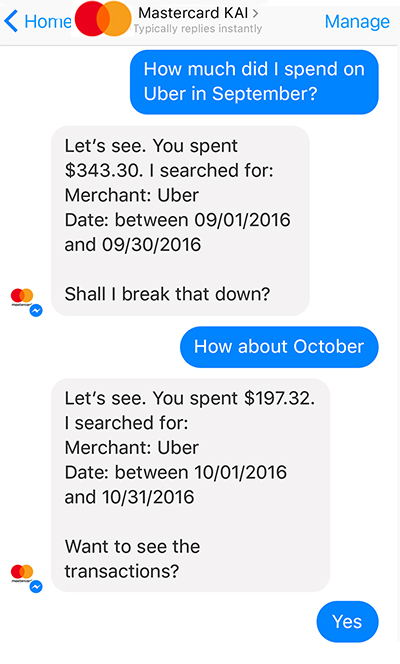
\includegraphics[scale=0.45]{Figures/mastercard.jpg}}
	\quad
	\subfloat[دستیار شخصی گوگل]{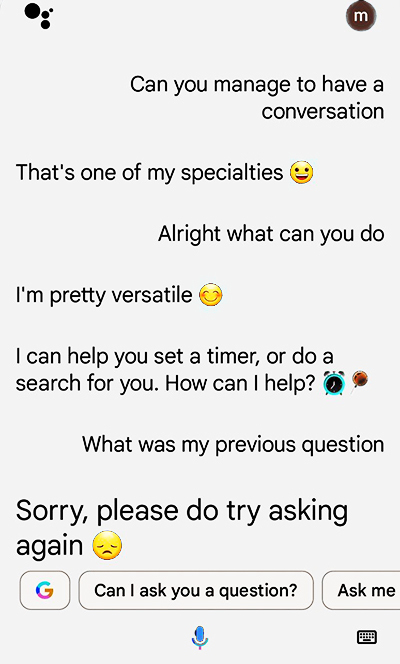
\includegraphics[scale=0.45]{Figures/assistant.jpg}}
	\caption{
		دستیار دیجیتال استفاده شده در وبسایت‌ها برای بهبود تجربه‌ی کاربری مشتریان
	}
	\label{Fig:DialoguesystemExamples۲}
\end{figure}
\\
\textbf {\ding{118} دستیار شخصی دیجیتال:}
دستیارهای شخصی دیجیتال، توانایی انجام کارهای روزمره مانند پخش موسیقی، تنظیم یادآور و کنترل ابزارهای هوشمند را دارند. بهره‌وری از این امکانات، منجر به افزایش کیفیت زندگی کاربران می‌شود. از نمونه‌های امروزی این دستیارها می‌توان به دستیار گوگل در شکل \ref{Fig:DialoguesystemExamples۲}، الکسا و سیری اشاره کرد.
\\
\textbf {\ding{118} دستیار شخصی خرید:}
این نوع از دستیارها در وبسایت‌های فروشگاهی به منظور فراهم کردن تجربه‌ی خرید بهتر برای کاربران مورد بهره‌وری قرار می‌گیرند. کاربر می‌تواند به جای ساعت‌ها گشتن در وبسایت برای یافتن محصول، با ارائه‌ی درخواست خود به دستیار خرید، سریع‌تر به محصول مورد نظرش برسد. چنین سیستمی قادر به ارائه پیشنهادهای ویژه به کاربر به منظور افزایش احتمال خرید او نیز هست. شکل \ref{Fig:DialoguesystemExamples} چنین سیستمی را در فروشگاه مایکروسافت و شرکت راه‌آهن امترک نمایش می‌دهد.
\\
\textbf {\ding{118} تدریس خصوصی برخط:}
این ابزار شامل یک سیستم گفت‌وگو برای تفسیر سوالات دانش‌آموزان و ارائه پاسخ‌های مناسب می‌باشد. قادر به ارائه راهنمایی و پشتیبانی شخصی به دانش آموزان است و می‌تواند به آن‌ها به منظور تسلط بر مطالعات خود کمک کند.
\begin{figure}[!htb]
	\centering
	\subfloat[دستیار دیجیتال فروشگاه مایکروسافت]{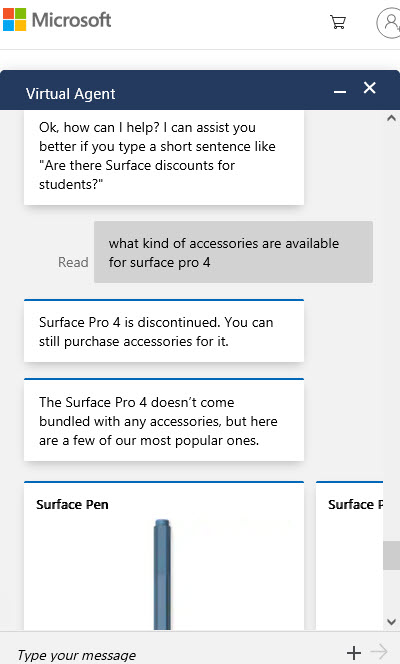
\includegraphics[scale=0.6]{Figures/microsoft.jpg}}
	\quad
	\subfloat[پشتیبان دیجیتال شرکت راه‌آهن امترک]{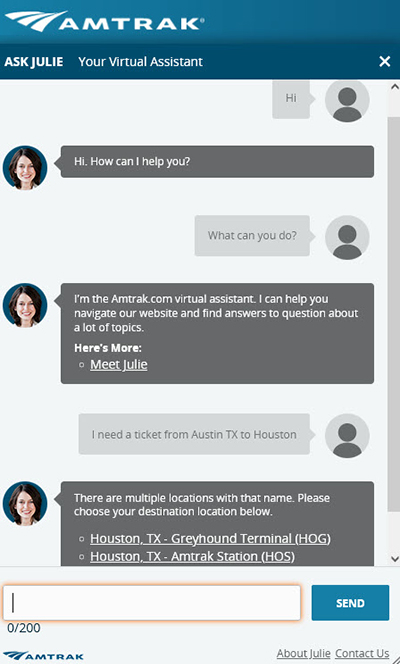
\includegraphics[scale=0.6]{Figures/amtrak.jpg}}
	\caption{
		دستیار دیجیتال استفاده شده در وبسایت‌ها برای بهبود تجربه‌ی کاربری مشتریان
	}
	\label{Fig:DialoguesystemExamples}
\end{figure}
\\
\textbf{\ding{118} تعامل در رسانه‌های اجتماعی:}
برای ارائه خدمات تعامل در شبکه‌های اجتماعی می‌توان از یک سیستم گفت‌وگو استفاده کرد. این سیستم قادر است سوالات مشتریان را در کانال‌های شبکه‌های اجتماعی تفسیر کرده و به شیوه‌ای مناسب به آن‌ها پاسخ دهد. همچنین، این سیستم می‌تواند واژه‌های کلیدی و عباراتی را که نشان‌دهنده احساسات مثبت یا منفی هستند، شناسایی کرده و به آن پاسخ دهد. از موارد پیاده‌سازی شده می‌توان به ربات شرکت تلوزیونی ام‌تی‌وی، و سامسونگ استرالیا نام برد \cite{socialchatbot}.

از طرف دیگر، مدلی که توانایی حل دو مسئله‌ی تشخیص هدف کاربر و استخراج روابط معنایی را بر داشته باشد، در بسیاری از وظایف دیگر پردازش زبان طبیعی نیز کاربرد دارد. همانطور که گفته شد، تشخیص هدف کاربر یک مسئله‌ی کلاس‌بندی است. از سایر وظایف کلاس‌بندی در زبان طبیعی که می‌توانند از معماری ارائه شده بهره ببرند، می‌توان به تحلیل احساسات\LTRfootnote{Sentiment Analysis}، تشخیص کلام نفرت‌افکن\LTRfootnote{Hate-Speech}، تشخیص اخبار جعلی\LTRfootnote{Fake-News Detection} و تشخیص موضع\LTRfootnote{Stance Detection} اشاره کرد. از سوی دیگر، مسئله‌ی پرکردن جای خالی یک مسئله‌ی برچسب‌زنی توالی است. سایر زمینه‌هایی که می‌توانند معماری مشترکی با این وظیفه داشته باشند شامل استخراج موجودیت، ابهام زدایی معنای واژه و برچسب زنی اجزاء سخن هستند. تشابه ساختار ورودی-خروجی و انتظارات مشابهی که از مدل زمینه‌های ذکرشده وجود دارد، باعث برجسته شدن فواید یک مدل قدرتمند در زمینه‌ی درک زبان طبیعی می‌شود.
\section{اهداف پژوهش}
به منظور آشنایی با محتوای پژوهش، باید با اهداف مورد نظر آن آشنا شد. در ادامه، اهدافی که این پایان‌نامه حول آن شکل گرفت معرفی می‌شوند.\\
\textbf{اول) }بسیاری از مدل‌های ارائه شده برای درک زبان طبیعی، همچنان از شبکه‌ی \lr{LSTM} به عنوان رمزنگار یا رمزگشا در مدل خود استفاده می‌کنند. نخستین هدف این پژوهش، ارائه‌ی مدلی است که شبکه‌های عصبی بازگشتی را کاملا کنار گذاشته و با ترنسفورمرها جابجا کند.\\
\textbf{دوم) }استفاده از ترنسفورمر، ضعف‌های ذاتی شبکه‌ی عصبی بازگشتی را پوشش می‌دهد. با این وجود شاید به نظر برسد که استفاده از شبکه‌ی عصبی کانولوشنی دیگر در رمزنگار ضروری نیست. هدف دوم پژوهش، بررسی عملکرد ترکیب شبکه‌ی عصبی بازگشتی، با ترنسفورمر در رمزنگار است.\\
\textbf{سوم) }تراز بودن مدل، موضوعی مهم در وظیفه‌ی برچسب زنی توالی است؛ اما تاکنون شیوه‌ای برای تراز کردن رمزگشای ترنسفورمر ارائه نشده است. هدف دوم پژوهش، ارائه کردن مدلی برای تراز کردن رمزگشای ترنسفورمر است.\\
\textbf{چهارم) }مدل زبانی بِرت انقلابی در یادگیری انتقالی در زبان طبیعی ایجاد کرد. پیش از برت، مدل زبانی اِلمو ارائه شده بود اما به اندازه‌ی برت مورد بررسی قرار نگرفت. علاوه بر این، تعداد کارهای اندکی در درک زبان طبیعی از المو استفاده کردند. در این کار قصد داریم عملکرد مدل زبانی المو را در شرایط یکسان، بر روی وظیفه‌ی درک زبان طبیعی بسنجیم. \\
\textbf{پنجم)} برخی از کارهای پیشین، مدل زبانی را به عنوان رمزنگار، و برخی دیگر به عنوان تعبیه‌ی کلمات استفاده کردند. یکی دیگر از اهداف این پژوهش، مقایسه‌ی این دو شیوه برای به کار گیری مدل زبانی است.\\
\textbf{ششم)} آخرین هدف در این پایان‌نامه، معرفی یک مدل جدید است که بر روی مجموعه داده‌ی \lr{SNIPS}‌ و یا \lr{ATIS}، بیشترین دقت را داشته باشد.
\section{ساختار پایان‌نامه}
در ادامه‌ی این پایان نامه، ابتدا در فصل ۲، به مفاهیم پایه‌ی درک زبان طبیعی و شبکه‌ی عصبی پرداخته می‌شود. در ادامه‌ی فصل ۲، مطالبی برای آشنایی با شبکه‌های عصبی ارائه می‌شود. سپس انواع شبکه‌های عصبی که در زمینه‌ی درک زبان طبیعی و وظایف مرتبط، از آن‌ها استفاده شده، معرفی می‌شوند. علت توصیف گسترده‌ی این شبکه‌ها، ماهیت کار این پایان‌نامه است؛ چراکه در این پایان‌نامه، یکی از کارهایی که صورت گرفته، تلاش برای پوشش ضعف شبکه‌های مورد استفاده است. در فصل ۳، یک دسته‌بندی کلی از کارهای پیشین در نظر گرفته شده، و در قالب این دسته‌بندی، پیشین مورد بررسی قرار گرفته‌اند. در فصل ۴،  مدل پیشنهادی این پایان‌نامه، یعنی \lr{CTran}، و اجزای سازنده‌ی آن معرفی شده‌اند. در فصل ۵، به تنظیمات به کار برده شده برای آموزش مدل، مجموعه داده‌های مورد استفاده، نتایج مدل پیشنهادی روی مجموعه داده‌ها و تجزیه و تحلیل نتایج پرداخته می‌شود. در فصل ۶، یک نتیجه‌گیری از آزمایش‌های صورت گرفته ارائه می‌شود. در پایان، کارهایی که می‌توان در آینده برای بهبود مدل پیشنهادی انجام داد، ذکر می‌شوند.



\chapter{ادبیات پژوهش}
\pagebreak
\section{مقدمه}
در فصل قبل، پیش‌درآمدی بر مسئله‌ی درک زبان طبیعی ارائه شد. از اهمیت مسئله سخن گفته و کاربرد آن در وظیفه‌های مختلف پردازش زبان طبیعی مطرح شد. به منظور بررسی روش‌ها و مدل‌های ارائه شده در این حوزه، آشنایی با مفاهیم پایه و همچنین اجزاء سازنده‌ی مدل‌ها لازم است. در فصل پیش رو به تعریف اصطلاحات و مفاهیم پایه پرداخته می‌شود. سپس، انواع شبکه‌های عصبی شده و شیوه‌های تعبیه‌ی واژه‌ها  معرفی می‌شوند.

\section{مفاهیم پایه}
در قسمت‌های مختلف این پایان‌نامه، اصطلاحاتی به کار برده شده که نیازمند روشنگری هستند. همچنین برخی از تعاریف مانند واژه و نشانه، مختص وظیفه‌ی درک زبان طبیعی هستند. در ادامه به معرفی ادبیات مورد استفاده در  این پایان نامه پرداخته می‌شود.
\textbf{یادگیری ماشین\LTRfootnote{Machine Learning}:}
یادگیری ماشین مجموعه‌ای از الگوریتم‌ها و مدل‌هایی است که به کامپیوتر اجازه می‌دهد بدون برنامه نویسی صریح، الگو و دانش را از داده‌ها استخراج کند. در یادگیری ماشین، کامپیوتر می‌تواند پیش‌بینی کرده یا تصمیم‌گیری کند. هدف اصلی در یادگیری ماشین، تولید الگوریتمی است که بتواند تصمیمات خود را به داده‌های جدید نیز تعمیم دهد. یادگیری ماشین به منظور کاهش یا به حداقل رساندن دخالت انسان، در وظایف مختلف استفاده می‌شود.
\\
\textbf{یادگیری باناظر\LTRfootnote{Supervised}:}
یادگیری باناظر شیوه‌ای از یادگیری ماشین است که از مجموعه داده‌ی برچسب گذاری شده، برای پیش‌بینی خروجی داده‌های جدید استفاده می‌کند. درواقع، در یادگیری باناظر از مجموعه داده‌ی آموزشی استفاده می‌کنند که حاوی پاسخ‌های صحیح است.
\\
\textbf{یادگیری خودناظر\LTRfootnote{Self-Supervised}:}
یادگیری خودناظر شاخه‌ای از یادگیری ماشین است که در آن، الگوریتم از خود داده‌ی آموزشی یاد می‌گیرد. در این شیوه، داده‌های آموزشی برچسب ندارند و الگوریتم باید از داده‌های آموزشی الگوها را استخراج کند.
\\
\textbf{سیستم گفت‌وگو:}
سیستم گفت‌وگو یک سیستم کامپیوتری است که برای شبیه‌سازی مکالمه با یک انسان به زبان طبیعی طراحی شده است. این سیستم می‌تواند اطلاعات را از طریق متن، گفتار\LTRfootnote{Speech}، لمس\LTRfootnote{Haptic} و تصاویر دریافت کند.
\\
\textbf{سیستم گفت‌وگوی هدف محور:}
نوعی از سیستم گفت‌وگو است که برای کمک به کاربر در دستیابی به یک هدف خاص طراحی شده است. این سیستم معمولاً مبتنی بر مجموعه‌ای از اهداف و شرایط از پیش تعریف شده است و از یک استراتژی تعریف شده برای هدایت کاربر به سمت آن اهداف استفاده می‌کند. سیستم گفت‌وگوی هدف محور برای انجام اهدافی مانند رزرو، سفارش محصولات و ارائه خدمات به مشتریان استفاده می‌شود.
\\
\textbf{درک زبان طبیعی:}
یک زمینه‌ی تحقیقاتی است که بر روی آموزش کامپیوترها، به منظور درک زبان انسان تمرکز دارد. برای این کار، کامپیوتر باید متن یا گفتار زبان طبیعی را دریافت کند و روابط معنایی\LTRfootnote{Semantic Relations} را از آن استخراج کند. این روابط شامل  تحلیل و درک نحو\LTRfootnote{Syntax}، معنا شناسی\LTRfootnote{Semantics} و عمل شناسی\LTRfootnote{Pragmatics} یک زبان است. این روابط با تعریف دو وظیفه\LTRfootnote{Task} استخراج می‌شوند؛ تشخیص هدف و تشخیص جای خالی.
\\
\textbf{تشخیص هدف:}
تشخیص هدف، فرآیند درک مقصود کلی\LTRfootnote{Overall Goal} از درخواست کاربر و تعیین هدف پشت آن است. هدف مشخص کننده‌ی عملی است که سیستم باید انجام دهد. به عنوان مثال، اگر کاربر بپرسد "آب و هوا امروز چگونه است؟" مقصود کلی کاربر آگاهی از آب و هوا، و هدف او به دست آوردن آب و هوای فعلی است. تشخیص هدف را می‌توان به‌عنوان طبقه‌بندی جمله‌ی کاربر، به دسته‌های از پیش تعیین‌شده تعریف کرد.
\\
\textbf{پر کردن جای خالی:}
پر کردن جای خالی، فرآیند استخراج اطلاعات مهم از جمله‌ی کاربر است که برای تکمیل درخواست کاربر، ضروری می‌باشد. این زیروظیفه شامل استخراج اطلاعات مرتبط مانند نام، تاریخ، مکان، اعداد، کدها، محصولات و غیره می‌شود. به عنوان مثال، اگر کاربر بپرسد "چه پروازهایی از لس آنجلس به نیویورک وجود دارد؟" وظیفه پر کردن جای خالی شامل استخراج مکان‌های لس آنجلس و نیویورک از ورودی کاربر است.
%\\
%\textbf{مجموعه داده\LTRfootnote{Dataset}:}
%مجموعه داده  به کلکسیونی از داده‌ها گفته می‌شود که برای آموزش و ارزیابی مدل‌های ارائه شده استفاده می‌شود. یک مجموعه داده  در حوزه‌ی زبان طبیعی، حاوی جملاتی به زبان طبیعی، برچسب‌های مربوط به هر واژه و یک کلاس به عنوان هدف کاربر است.
\\
\textbf{واژه\LTRfootnote{Word}:}
واژه در حوزه‌ی کاری درک زبان طبیعی، به معنای مجموعه‌ای از حروف و اعداد است که توسط یک جداکننده (فاصله‌ی خالی)\LTRfootnote{White Space} از یکدیگر جدا شده‌اند. واژه می‌تواند شامل ترکیبی از حروف معنی‌دار یا ترکیبی از حروف، اعداد و علائمی باشد که حاوی اطلاعات است.
\\
\textbf{نشانه\LTRfootnote{Token}:}
از آنجا که نمی‌توان واژه‌های زبان طبیعی را مستقیما وارد شبکه‌ی عصبی کرد، ابتدا واژه را به نشانه تبدیل می‌کنند. در این فرایند، ممکن است واژه به اجزاء سازنده‌اش شکسته شود تا پیدا کردن روابط معنایی میان واژه‌ها برای شبکه ساده‌تر شود. سپس برای هر نشانه‌ی یکتا، یک شماره‌ی یکتا در نظر گرفته می‌شود. به فرایند شکستن واژه‌ها نشان کردن\LTRfootnote{Tokenize} و به شماره‌ی یکتای نشان، شناسه‌ی نشان\LTRfootnote{Token ID} می‌گویند. 


\section{شبکه‌ی عصبی}
شبکه‌ی عصبی یکی از روش‌های یادگیری ماشین بوده که نقشی محوری در یادگیری عمیق ایفا می‌کند. این شبکه بر اساس مشاهدات قبلی، ضمن تشخیص الگوهای موجود، نسبت به چالش پیش روی خود تصمیم‌گیری کرده و پیش‌بینی‌های مورد نظر را انجام می‌دهد. منظور از مشاهدات قبلی، داده‌هایی است که شبکه در طول فرایند آموزش با آن برخورد داشته است. به منظور بررسی صحیح عملکرد، این داده‌ها نباید با سایر داده‌هایی که برای فرایند آزمایش استفاده می‌شوند اشتراکی داشته باشند.
شبکه‌ی تغذیه‌به‌جلو نوعی شبکه‌ی عصبی مصنوعی است که اتصالات میان گره‌های آن تشکیل حلقه نمی‌دهد. در شبکه‌ی تغذیه‌به‌جلو، اطلاعات فقط از یک سمت جریان دارد؛ اطلاعات از گره‌های ورودی وارد شبکه شده، از لایه‌ی مخفی گذر کرده و به سمت گره‌های خروجی می‌رود. شکل \ref{Fig:MLP}، نوعی از شبکه‌ی عصبی تغذیه‌به‌جلو به نام شبکه‌ی تماماً متصل را ترسیم می‌کند. در این شبکه، گره‌ها در لایه‌های متفاوت قرار می‌گیرند. گره‌های یک لایه هیچ‌گونه اتصال مستقیمی به یکدیگر ندارند و گره‌های هر لایه، توسط وزن‌ها به گره‌های لایه‌ی بعد متصل می‌شوند. فرایند یادگیری در شبکه، توسط الگوریتم پس‌انتشار\LTRfootnote{Back-Propagation} صورت می‌گیرد. این الگوریتم، ابتدا داده‌های ورودی را به شبکه تغذیه کرده و سپس خطای شبکه را با محاسبه‌ی فاصله‌ی بین خروجی تولید شده و خروجی واقعی به دست می‌آورد. پس از آن،  خطا به عقب در شبکه منتشر می‌شود و وزن‌ها را با توجه به بزرگی خطا تنظیم می‌کند. فرایند تنظیم وزن‌ها با استفاده از یک الگوریتم بهینه سازی\LTRfootnote{Optimization Algorithm} انجام می‌شود که وزن‌ها را در جهتی تنظیم می‌کند که خطا را به حداقل برساند. از میان الگوریتم‌های شناخته شده‌ی بهینه‌سازی، می‌توان به کاهش گرادیان\LTRfootnote{Gradient Descent}، کاهش گرادیان تصادفی و آدام اشاره کرد.
\\
شبکه‌ی تماماً متصل چند لایه، برای کاربردهای کلاس‌بندی که ورودی آن‌ها یک بردار باشد، سودمند است؛ اما در صورتی که اطلاعات مورد نظر حاوی ترتیب باشند، امکان نگهداری اطلاعات ترتیبی مربوط به بردارها وجود ندارد.
 \begin{figure}[!htb]
 	\centering
 	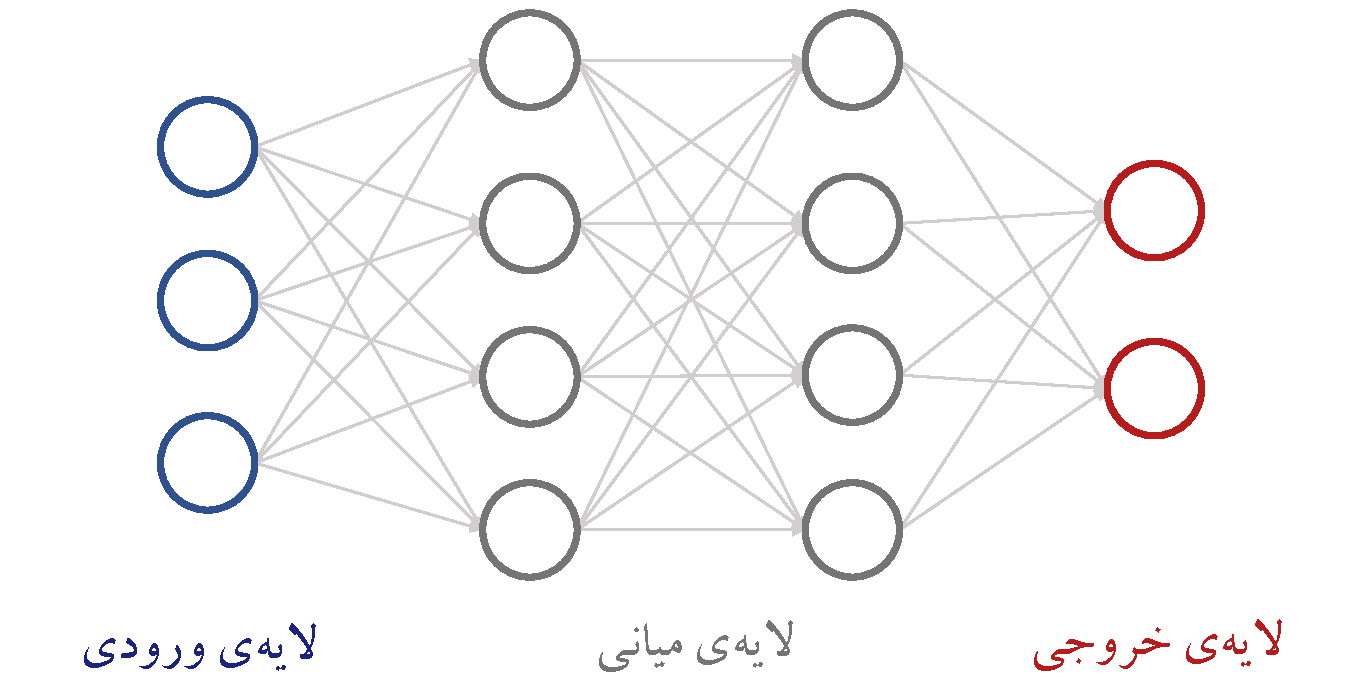
\includegraphics[scale=0.4]{Figures/neuralnet.pdf}
 	\caption[شبکه‌ی عصبی تماماً متصل با دو لایه‌ی میانی]{شبکه‌ی عصبی تماماً متصل با دو لایه‌ی میانی. هرکدام از لایه‌های ورودی، میانی و خروجی با رنگ یکتا  متمایز شده‌اند.}
 	\label{Fig:MLP}
 \end{figure}



\section{شبکه‌ی عصبی بازگشتی}
شبکه‌ی عصبی بازگشتی نوعی شبکه‌ی عصبی است که اتصالات میان گره‌های آن، حلقه تشکیل می‌دهند. درواقع، گره‌ها به نحوی به هم متصل هستند که به شبکه امکان به خاطر سپردن ورودی‌های گذشته را می‌دهد. به خاطر سپردن، این امکان را برای شبکه محیا می‌کند که تصمیمات آینده‌ی آن، وابسته به ورودی‌های پیشین نیز بشود \cite{rnn}. بدین ترتیب، خروجی شبکه می‌تواند حاصل ترتیبی از رویدادها باشد که در قالب بردار درآمده‌اند. از این رو، ورودی‌های یک شبکه‌ی عصبی بازگشتی، بصورت ترتیبی است. به عبارت دیگر ترتیب ورودی، خود دارای معنا و مفهوم است و باید ضمن دادن ورودی‌ها به شبکه، این مفهوم حفظ شود. بطور مثال جریان صدا، فریم‌های تصویر(فیلم)، و متن زبان طبیعی می‌توانند از شبکه‌های عصبی بازگشتی بهره ببرند. به این نوع ورودی‌ها، سری‌های زمانی\LTRfootnote{Time Series} نیز می‌گویند.
 \begin{figure}[!htb]
	\centering
	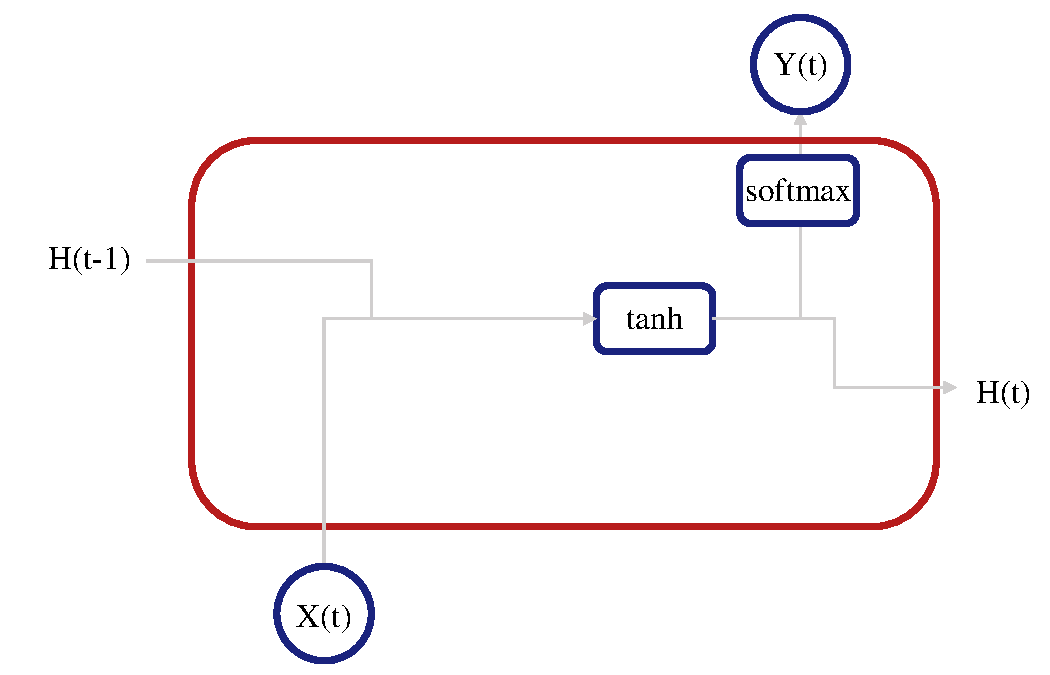
\includegraphics[scale=0.6]{Figures/RNN.pdf}
	\caption{یک بلوک از شبکه‌ی عصبی بازگشتی}
	\label{Fig:RNNBlock}
\end{figure}

شکل \ref{Fig:RNNBlock} معماری شبکه‌ی عصبی بازگشتی را نمایش می‌دهد. در معماری این نوع شبکه‌ها، علاوه بر بردار ورودی شبکه $X_{(i)}$، بردار حالت مخفی\LTRfootnote{ُHidden State} $H_{(i-1)}$  از مرحله‌ی قبلی شبکه نیز به عنوان ورودی به آن داده می‌شود. برای ورودی شبکه، وزن‌های بردار ورودی $W_{x}$ و برای بردار حالت مخفی، وزن‌های بردار حالت مخفی $W_{h}$، جداگانه در نظر گرفته می‌شود. بدین ترتیب، بردار حالت مخفی هر مرحله از طریق معادله‌ی \ref{Eq:RNNBlockHidden} و بردار خروجی از طریق معادله‌ی \ref{Eq:RNNBlockOutput} محاسبه می‌شود.
\begin{equation}
	H_{t} = tanh(W_{x}.X(t) + W_{h}.X(t-1) + b_{h})
	\label{Eq:RNNBlockHidden}
\end{equation}\vspace{-\baselineskip}
\begin{equation}
	Y_{t} = softmax(W_{Y}.H_{t} + b_{Y})
	\label{Eq:RNNBlockOutput}
\end{equation}
در معادلات فوق، $W_{Y}, W_{H}, b_{h}, b_{Y}$ همگی پارامترهای قابل آموزش هستند.


 \begin{figure}[!htb]
	\centering
	\includegraphics[scale=0.7]{Figures/RNNenrolled.pdf}
	\caption[شبکه‌ی عصبی بازگشتی گسترده شده در بعد زمان]{شبکه‌ی عصبی بازگشتی گسترده شده در بعد زمان. در این شکل هر بلوک بیانگر یک گام زمانی است.}
	\label{Fig:RNNenrolled}
\end{figure}
برای استفاده از شبکه‌ی عصبی بازگشتی در کاربرد پردازش متن، مطابق شکل \ref{Fig:RNNenrolled}، در هر گام زمانی\LTRfootnote{Time-Step}، یک واژه به همراه بردار حالت مخفی قبل به شبکه داده می‌شود. بردار تولید شده‌ی $Y_{(t)}$ به عنوان خروجی شبکه در گام زمانی $t$ و بردار $H_{(t)}$ به عنوان بردار حالت مخفی به گام زمانی بعد داده می‌شود. با چنین ساختار شبکه‌ای، می‌توان ورودی با طول پویا به شبکه داد.


برای استفاده‌ی شبکه‌ی عصبی بازگشتی در وظیفه‌هایی مانند ترجمه، عموماً از معماری رمزنگار - رمزگشا استفاده می‌کنند. در رمزنگار، ورودی شبکه‌ی عصبی تبدیل به یک بردار می‌شود. این بردار در گام بعد، وارد رمزگشا می‌شود تا نشانه‌های مورد نظر را تولید کند. شکل \ref{Fig:RNNenrolled}، مورد استفاده‌ی شبکه‌ی عصبی بازگشتی در رمزنگار را توضیح می‌دهد. شکل \ref{Fig:RNNdecoderenrolled} شیوه‌ی استفاده از شبکه عصبی بازگشتی در رمزگشا را به تصویر می‌کشد. در بخش رمزگشا، از آنجایی که نشانه‌های صحیح موجود نیست، نشانه‌ای قراردادی مانند $(BOS)$\LTRfootnote{Beggining of Sentence} را به عنوان اولین نشانه وارد شبکه می‌کنند. سپس در هر گام زمانی، نشانه‌ی تولید شده توسط مدل به عنوان ورودی مرحله‌ی بعد استفاده می‌شود. این کار تا زمانی تکرار می‌شود که نشانه‌ای قراردادی مانند $(EOS)$\LTRfootnote{End Of Sentence} تولید شود.
 \begin{figure}[!htb]
	\centering
	\includegraphics[scale=0.7]{Figures/RNNdecoderenrolled.pdf}
	\caption[شبکه‌ی عصبی بازگشتی در نقش رمزگشا، گسترده شده در بعد زمان]{شبکه‌ی عصبی بازگشتی در نقش رمزگشا، گسترده شده در بعد زمان. در این شکل هر بلوک بیانگر یک گام زمانی است.}
	\label{Fig:RNNdecoderenrolled}
\end{figure}

یک شبکه عصبی بازگشتی از نظر تئوری باید قادر به تولید دنباله‌هایی با هر پیچیدگی ای باشد اما در عمل مشاهده می‌کنیم که اگر تعداد گام زمانی در چنین شبکه‌ای به اندازه کافی زیاد باشد، در ذخیره سازی اطلاعات مرتبط با ورودی‌های قبلی به مدت طولانی ناتوان است \cite{RNNGradientProblem}.
علاوه بر اینکه این خصیصه توانایی شبکه را در مدل سازی ورودی‌های طولانی تضعیف می‌کند، باعث می‌شود که شبکه در زمان تولید دنباله‌ای از کلمات، در معرض ناپایداری قرار بگیرد. مشکلی که وجود دارد این است که اگر پیش‌بینی‌های شبکه تنها وابسته به چند ورودی اخیر باشد و این ورودی ها خود نیز توسط شبکه تولید شده باشند، شانس بسیار کمی برای تصحیح و جبران اشتباهات گذشته توسط شبکه وجود دارد. به طور مثال اگر ترجمه‌ی یک واژه در ابتدای جمله، به واژه‌ای در انتهای جمله وابسته باشد، و جمله‌ی یاد شده طولانی هم باشد، ممکن است شبکه نتواند به خوبی عمل کند. علت این امر دو مسئله‌ی گرادیان محو شونده\LTRfootnote{Vanishing Gradient} و گرادیان انفجاری\LTRfootnote{Exploding Gradient} است \cite{VanishingGradient}.
\\
انواع مختلفی از شبکه‌های عصبی بازگشتی وجود دارد؛ بطور مثال \lr{GRU} و \lr{LSTM} . از آنجا که در اکثر کاربرد‌های زبان طبیعی شبکه‌ی \lr{LSTM} مورد استفاده قرار می‌گیرد، تنها به معرفی این معماری پرداخته می‌شود.

\section{حافظه‌ی کوتاه‌مدت طولانی}
داشتن یک حافظه بلند مدت شبکه را به ثبات بیشتری می‌رساند؛ چراکه اگر شبکه بتواند از تاریخچه‌ی خود درک صحیحی پیدا کند، می‌تواند با مشاهده‌ی ورودی‌های ابتدایی، پیش‌بینی بهتری ارائه کند. شبکه‌ی حافظه‌ی کوتاه‌مدت طولانی\LTRfootnote{Long Short-Term Memory (LSTM)}، با معرفی سلول حافظه\LTRfootnote{Memory Cell} قادر است نسبت به حفظ حافظه فعلی از طریق دروازه‌های معرفی شده تصمیم‌گیری کند \cite{lstm}. ازنظر شهودی، اگر واحد \lr{LSTM} داده‌ی مهمی در دنباله ورودی را در گام‌های ابتدایی تشخیص دهد، با استفاده از دروازه‌های معرفی شده می‌تواند این اطلاعات را طی گام‌های زمانی بعدی نیز منتقل کند. بدین ترتیب، \lr{LSTM} می‌تواند این گونه وابستگی‌های بلندمدت را دریافت کرده و حفظ دارد. در ادامه به معرفی این دروازه‌ها پرداخته می‌شود.


 \begin{figure}[!htb]
	\centering
	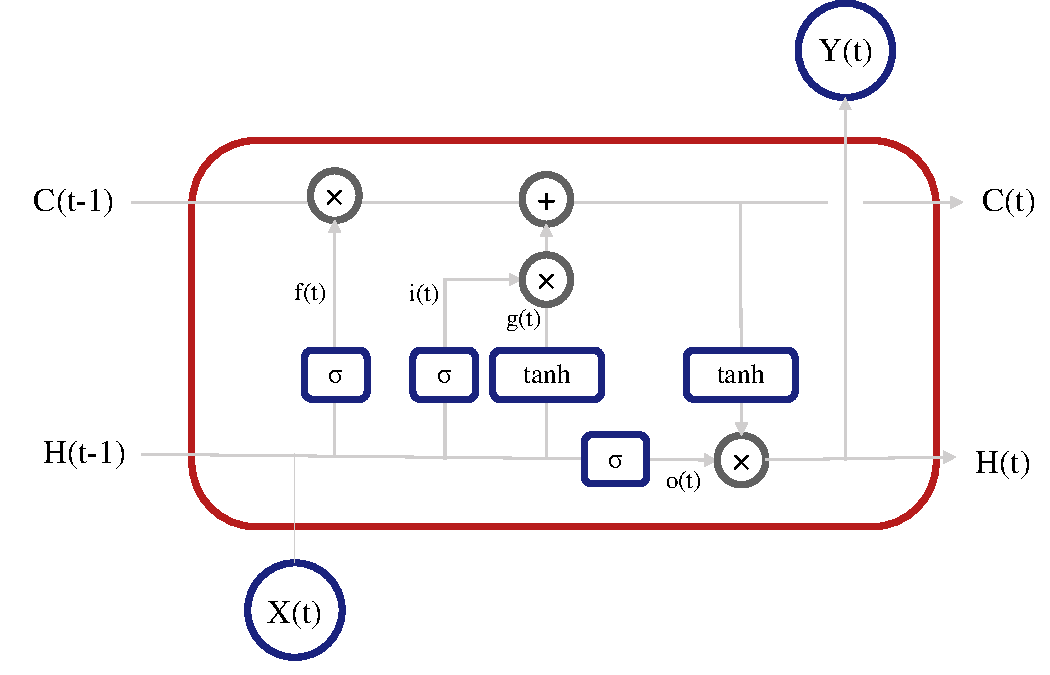
\includegraphics[scale=0.6]{Figures/LSTM.pdf}
	\caption{یک بلوک از حافظه کوتاه‌مدت طولانی}
	\label{Fig:LSTMBlock}
\end{figure}
شکل \ref{Fig:LSTMBlock} ساختار درون یک بلوک \lr{LSTM} را به‌تصویر می‌کشد. معماری \lr{LSTM}‌ دارای ۳ دروازه است؛ دروازه‌ی ورودی\LTRfootnote{Input Gate}، دروازه‌ی فراموشی\LTRfootnote{Forget Gate} و دروازه‌ی خروجی\LTRfootnote{Output Gate}.
این سه دروازه با همکاری یکدیگر حافظه‌ی فعلی سلول $C_{t}$ را بروزرسانی و حالت فعلی شبکه $H_{t}$ را تعیین می‌کنند.  
معادله‌ی \ref{Eq:LSTMForget} دروازه‌ی فراموشی $f_{t}$ را نشان می‌دهد. این دروازه مشخص می‌کند چه میزان از اطلاعات قبلی باید دور ریخته شود.
\begin{equation}
	f_{t} = σ(W_{f}.[H_{t-1},X_{t}] + b_{f})
	\label{Eq:LSTMForget}
\end{equation}
در این رابطه $σ$ تابع فعال ساز و $W$ و $b$ هردو پارامترهای قابل آموزش هستند. معادله‌ی \ref{Eq:LSTMInput} بیانگر دروازه‌ی ورودی است. این دروازه مشخص می‌کند چه میزان از اطلاعات ورودی در گام زمانی فعلی باید در حافظه‌ی فعلی سلول ذخیره شود.
\begin{equation}
	i_{t} = σ(W_{i}.[H_{t-1},X_{t}] + b_{i})
	\label{Eq:LSTMInput}
\end{equation}
معادله‌ی \ref{Eq:LSTMOutput} نشانگر دروازه‌ی خروجی است. دروازه‌ی خروجی مشخص می‌کند که با توجه به سلول حافظه $C_{t}$، چه چیزی در خروجی قرار گیرد.
\begin{equation}
	o_{t} = σ(W_{o}.[H_{t-1},X_{t}] + b_{o})
	\label{Eq:LSTMOutput}
\end{equation}
به همین ترتیب، حالت فعلی سلول حافظه ازطریق معادله‌ی \ref{Eq:LSTMCt} به دست می‌آید. در این معادله، $⊙$ بیانگر ضرب نقطه‌ای\LTRfootnote{Dot Product} است.
\begin{equation}
	\begin{array}{l}
		q_{t} = tanh(W_{q}.[H_{t-1},X_{t}] + b_{q})\\
		C_{t} = f_{t} ⊙ C_{t-1} + i_{t} ⊙ q_{t}
	\end{array}
	\label{Eq:LSTMCt}
\end{equation}
در آخر، حالت مخفی $H_{t}$ و خروجی $Y_{t}$ در زمان $t$، توسط معادله‌ی \ref{Eq:LSTMHt} محاسبه می‌شود.
\begin{equation}
	\begin{array}{l}
		H_{t} = o_{t} ⊙ tanh(C_{t})\\
		Y_{t} = softmax(H_{t}) 
	\end{array}
	\label{Eq:LSTMHt}
\end{equation}
\subsection{حافظه‌ی کوتاه‌مدت طولانی دوطرفه}
تا کنون، پیش‌فرض استفاده از \lr{LSTM} برای تعبیه‌ی کلمات به صورت ترتیبی و در یک جهت بود. اما در زبان طبیعی، وابستگی‌های معنایی دوطرفه هستند؛ به این معنا که تعبیه‌ی یک واژه می‌تواند علاوه بر وابستگی به واژه‌ی پیشین، به واژه‌ی بعد از خود نیز وابسته باشد. از این رو، بنظر می‌رسد که معماری اولیه‌ی \lr{LSTM} این نیاز را برطرف نمی‌کند. یکی از راهکارهایی که برای حل این مسئله ارائه کردند در شکل \ref{Fig:BILSTM} ترسیم شده است.


 \begin{figure}[!htb]
	\centering
	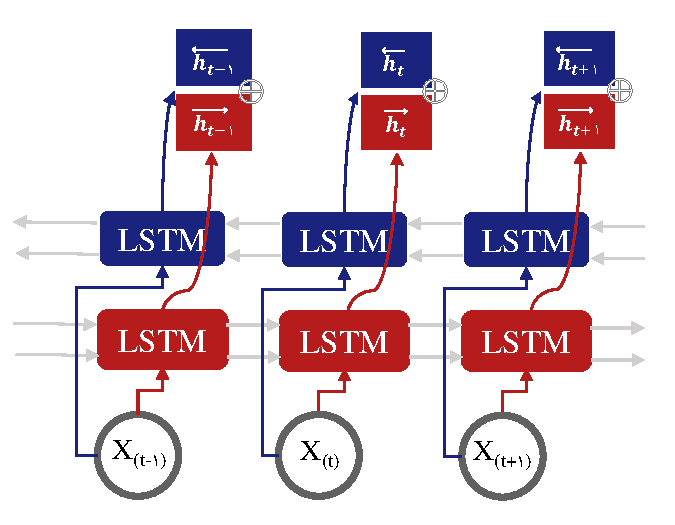
\includegraphics[scale=0.7]{Figures/bilstmenrolled.pdf}
	\caption[شبکه‌ی \lr{LSTM} دوطرفه]{شبکه‌ی \lr{LSTM} دوطرفه، گسترده شده در بعد زمان.}
	\label{Fig:BILSTM}
\end{figure}
شکل \ref{Fig:BILSTM}، یک \lr{LSTM} دوطرفه را نشان می‌دهد که در بعد زمان گسترده شده است. در \lr{LSTM} دوطرفه، یک لایه‌ی \lr{LSTM}، ابتدا از سمت چپ به راست $\overset{\rightarrow}{h}$، و سپس لایه‌ای دیگر از سمت راست به چپ $\overset{\leftarrow}{h}$، توالی واژه‌ها را پردازش می‌کند. تعبیه‌ی حاصل به دست آمده از این دو عملیات، با یکدیگر الحاق $\oplus$ می‌شوند تا تعبیه‌ی پایانی دوطرفه $(\overset{\rightarrow}{h}\oplus \overset{\leftarrow}{h})$ برای واژه ساخته شود.
\subsection{مکانیزم توجه}
روش دیگری که برای بهبود عملکرد شبکه‌ی \lr{LSTM} استفاده می‌شود، مکانیزم توجه \cite{attention_bahdanau} است. مکانیسم توجه به شبکه اجازه می‌دهد هنگام تصمیم گیری برای تولید هر نشانه، روی بخش‌های خاصی از ورودی تمرکز کند. این کار، با تخصیص وزن‌های مختلف به هر عنصر در دنباله ورودی انجام می شود. بدین ترتیب، مکانیزم توجه به عناصری که برای تصمیم گیری اهمیت بیشتری دارند وزن بیشتری می‌دهد. برداری که حاوی وزن‌ها است، بردار توجه نامیده می‌شود. این بردار توجه، به عنوان بخشی از ورودی، وارد شبکه‌ی \lr{LSTM} می‌شود. شیوه‌ی وارد کردن این بردار، الحاق آن با بردار تعبیه‌ی ورودی است. شکل \ref{Fig:attenbahdanau} شیوه‌ی محاسبه‌ی مکانیزم توجه را نشان می‌دهد.
 \begin{figure}[!htb]
	\centering
	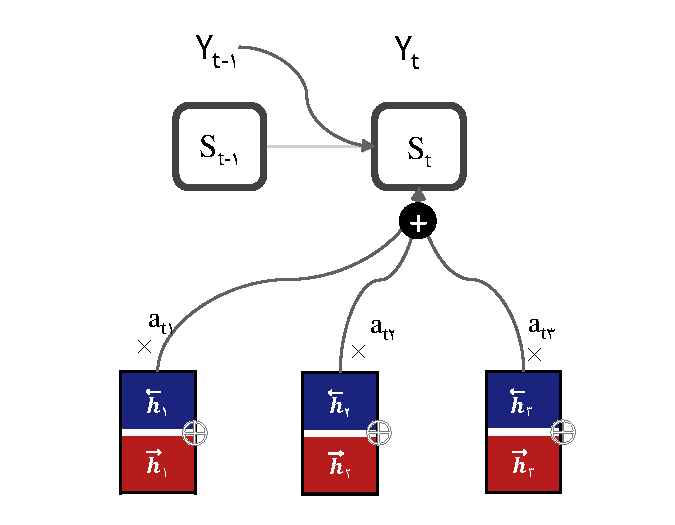
\includegraphics[scale=0.7]{Figures/bahdanauattention.pdf}
	\caption[مکانیزم توجه]{مکانیزم توجه تعریف شده در \cite{attention_bahdanau}.}
	\label{Fig:attenbahdanau}
\end{figure}


در واقع، در یک شبکه‌ی رمزگشای \lr{LSTM} که از مکانیزم توجه بهره می‌برد، حالت مخفی در هر مرحله‌ی زمانی، تابعی از حالت مخفی قبلی $S_{t-1}$، خروجی تولید شده‌ی قبلی $Y_{t-1}$ و بردار توجه $C_{t}$ است. این تابع را به صورت $s_{i}=f(S_{t-1},Y_{t-1},C_{t})$ نمایش می‌دهند. لازم به ذکر است که در این معادله، مقدار $C_{t}$ به ازاء هر واژه در خروجی متفاوت است. برای محاسبه‌ی $C_{t}$، جمع وزن‌داری از تمام حالت مخفی‌های رمزنگار ایجاد می‌شود، که وزن آن در طول فرایند یادگیری تغییر می‌کند. معادله‌ی \ref{Eq:atten_bahdanau} شیوه‌ی محاسبه‌ی $C_{t}$ را نمایش می‌دهد.
\begin{equation}
	c_{t}=\sum_{j=1}^{T_{x}}a_{tj}h_{j}
	\label{Eq:atten_bahdanau}
\end{equation}
در معادله‌ی \ref{Eq:atten_bahdanau}، $a_{tj}$ ماتریس متغیر قابل آموزش، به اندازه‌ی طول توالی ورودی $T_{x}$ در طول توالی خروجی $T_{y}$ است.
ماتریس توجه برای همه‌ی موقعیت‌ها، درواقع متغیر بوده و در طول فرایند آموزش مدل در وظیفه‌ی مورد نظر، تغییر می‌کند. از این رو، وزن‌های بردار توجه برای هر نوع وظیفه‌ی پردازش زبان طبیعی، متفاوت است.
\subsection{ضعف ذاتی}
با وجود برتری شبکه‌ی \lr{LSTM} در برابر شبکه‌ی بازگشتی، چالش‌هایی برای استفاده از این شبکه نیز وجود دارد. با توجه به این که پارامترهای شبکه‌ی \lr{LSTM}‌ نسبت به شبکه‌ی بازگشتی بسیار بیشتر است، آموزش آن و همگرا شدن شبکه نیازمند زمان و داده‌های بیشتری است. همچنین، \lr{LSTM} همیشه نمی‌تواند ظرافت‌های موجود در یک متن را درک کند. در ادامه، \lr{LSTM}‌ با وجود بهبود عملکرد شبکه‌ی بازگشتی، پوششی کوچک بر ضعف‌های ذاتی این نوع شبکه ایجاد کرده‌است \cite{info12110442}؛ اما ضعف ذاتی همچنان وجود دارد و نمی‌توان عملکردی مناسب در ترتیب‌های بزرگ دید \cite{VanishingGradient,Kag2020RNNs}. از طرف دیگر، به‌خاطر ورود ترتیبی بردارها به شبکه و پردازش سلسله مراتبی اطلاعات، نمی‌توان به خوبی از ظرفیت سخت‌افزارهای امروزی که قابلیت پردازش موازی و سریع داده‌ها را دارند بهره ‌برد. با توجه به مسائل ذکر شده، احتیاج به شبکه‌ای با پوشش واقعی این ضعف‌ها وجود دارد.
\section{شبکه‌ی عصبی کانولوشنی}

شبکه عصبی کانولوشنی\LTRfootnote{Convolutional Neural Network (CNN)} از یک لایه ورودی، لایه‌های پنهان و یک لایه خروجی تشکیل شده است. 
 در هر عملیات کانولشن، یک ماتریس هسته و یک ماتریس ورودی وجود دارد. ماتریس هسته\LTRfootnote{Kernel} که به آن فیلتر نیز می‌گویند، با حرکت روی ماتریس ورودی و ضرب نقطه‌ای مقادیر دو ماتریس که در معادله‌ی  \ref{Eq:Convolution} تعریف شده است، ماتریس خروجی را تولید می‌کند. به ماتریس تولید شده نقشه‌ی ویژگی\LTRfootnote{Feature Map} می‌گویند. 
 \begin{equation}
 	c=A\left(x\odot f+b\right)
 \label{Eq:Convolution} 
\end{equation}
در معادله‌ی فوق که عملیات کانولوشن را نشان می‌دهد، ورودی $x$، هسته $f$ و تابع فعال‌ساز $A$، و عملیات کانولوشن با $c$ برابر است.\\
حرکت هسته بر روی ماتریس ورودی می‌تواند همراه با پرش باشد، به این معنا که از محاسبه‌ی برخی از پنجره‌های ممکن صرف نظر شده و پنجره‌ی بعدی را محاسبه می‌شود. به پارامتر تعیین کننده‌ی پرش پنجره، گام\LTRfootnote{Stride} می‌گویند. در صورتی که از پد\LTRfootnote{Pad} استفاده نشود، ابعاد ماتریس ویژگی کوچک‌تر از ماتریس ورودی می‌شود. پد در شبکه‌ی کانولوشنی به معنای ایجاد موقعیت‌های جدید در ماتریس، با مقادیر ازپیش تعریف شده است. این مقادیر از پیش تعریف شده می‌تواند با توجه به سیاست خاصی از اعداد درون ماتریس انتخاب شود یا عدد مشخصی مانند صفر درون آن قرار گیرد. همچنین استفاده از گام بزرگتر از ۱ باعث کوچکی ماتریس ویژگی می‌شود. اندازه‌ی خروجی را می‌توان با استفاده از معادله‌ی \ref{Eq:ConvolutionDimension} محاسبه کرد. در این معادله، گام با $S$ اندازه‌ی ورودی با $N$، اندازه‌ی هسته با $M$، اندازه‌ی پد با $P$ و اندازه‌ی خروجی با $O$ مشخص شده است.
  \begin{equation}
 	O=\frac{N - \left(M-1\right)+P}{S}
 	\label{Eq:ConvolutionDimension} 
 \end{equation}
ورودی شبکه‌ی کانولوشنی می‌تواند به اندازه‌ی دلخواه بعد داشته باشد. برای هر بعد می‌توان با استفاده از معادله‌ی \ref{Eq:ConvolutionDimension}، اندازه‌ی خروجی را محاسبه کرد. شکل \ref{Fig:CNN} انجام عملیات کانولوشن یک هسته بر روی یک ماتریس را نمایش می‌دهد. برای سادگی در نمایش، کانال ورودی برابر ۱ در نظر گرفته شده است. لازم به ذکر است که کانال ورودی همواره با کانال هسته برابر است. در صورتی که کانال ورودی بزرگتر از ۱ باشد، مقدار هسته در هر کانال متفاوت با دیگری‌است.
 \begin{figure}[!htb]
	\centering
	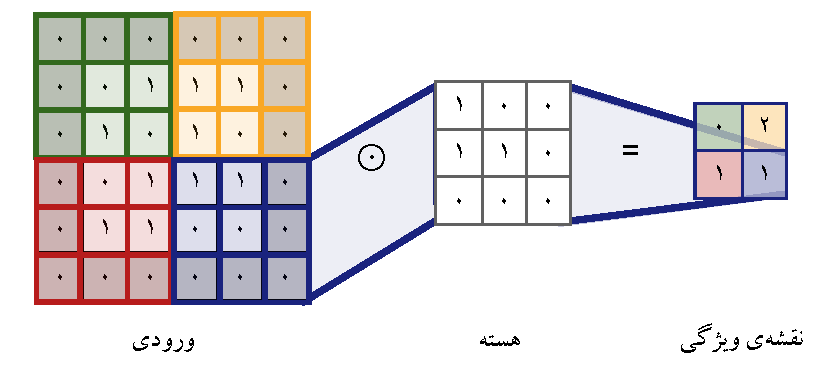
\includegraphics[scale=1]{Figures/cnn.pdf}
	\caption[کانولوشن یک هسته بر روی ماتریس ورودی]{
کانولوشن یک هسته بر روی ماتریس ورودی. در این شکل، هسته دارای طول ۳، عرض ۳ و کانال ۱ و ماتریس ورودی دارای طول ۳، عرض ۳ و کانال ورودی برابر۱ است. در این عملیات گام برابر با ۳ و پد برابر ۲ در نظر گرفته شده است. همچنین، رنگ خاکستری نمایانگر پد بوده و هر رنگ سبز، زرد، قرمز و آبی برابر با یک پنجره است.}
	\label{Fig:CNN}
\end{figure}

برای هر ورودی، یک بعد به عنوان تعداد کانال ورودی در نظر گرفته می‌شود. بعد از پایان اعمال یک هسته بر روی ورودی، آن بعد تبدیل به ۱ می‌شود. به عنوان مثال، در صورتی که ابعاد ورودی $(Height,Width,D)$ بوده، با فرض استفاده از پد، تعداد کانال ورودی برابر $D$، و و استفاده از یک هسته، خروجی برابر با $(Height,Width,1)$ می‌شود. اما عملیات کانولوشن می‌تواند با چند هسته و با مقادیر اولیه‌ی مختلف برای هسته‌ها تکرار شود. بدین ترتیب، در صورتی که از تعداد $K$ هسته استفاده شود، خروجی برابر با $(Heigh,Width,K)$ خواهد شد.
  در صورتی که شبکه‌ی کانولوشنی به صورت لایه‌ای باشد، نقشه‌ی ویژگی هر لایه، برای لایه‌ی مرحله‌ی بعد استفاده می‌شود. در لایه‌های بعد از لایه‌ی کانولوشن، معمولاً لایه‌های ادغامی\LTRfootnote{Pooling}، لایه‌های کاملاً متصل و لایه‌های نرمال‌سازی قرار می‌گیرند.
 \section{میدان تصادفی شرطی زنجیره‌ی خطی}
 میدان تصادفی شرطی\LTRfootnote{Conditional Random Field (CRF)}  زنجیره خطی، نوعی مدل گرافیکی احتمالی است که ابزار قدرتمندی برای مدل‌سازی و پیش‌بینی روابط بین متغیرها در یک دنباله می‌باشد. مانند سایر \lr{CRF}ها، \lr{CRF} زنجیره خطی هم، برای وظایف یادگیری با ناظر و هم بدون نظارت مانند طبقه بندی، تقسیم بندی\LTRfootnote{Segmentation} و برچسب گذاری استفاده می‌شود. \lr{CRF} زنجیره خطی، به ویژه برای کارهایی که شامل داده‌های متوالی هستند، مانند پردازش زبان طبیعی مفید است. اگرچه در هیچ کجای معماری پیشنهادی، از \lr{CRF}  استفاده نشده است، اما بخاطر به استفاده‌ی برخی از مدل‌های پیشین از آن، در این بخش به طور خلاصه معرفی می‌شود.
 
با در نظر گرفتن بردار خروجی رمزنگار برای وظیفه‌ی تشخیص جای خالی $Y=\{y_{1},y_{2},\cdots ,y_{N}\}$، توالی برچسب‌های جای خالی $s=\{s_{1},s_{2},\cdots ,s_{N}\}$ و تمام توالی‌های برچسب ممکن برای $s$ به عنوان $S(y)$، یک \lr{CRF} احتمال وقوع دنباله‌ی ترتیبی $s$ را در صورت مشاهده‌ی ورودی $y$، به ازای تمام $s$های ممکن، با معادله‌ی \ref{Eq:CRF} محاسبه می‌کند.
 \begin{equation}
 	p(s|y;W,b)=\frac{\prod_{i=1}^{N}e^{W^{T}_{s_{i-1},s_{i}}y_{i}+b_{s_{i-1},s_{i}}}}{\sum_{s^{\prime}\in S(y)}^{}\prod_{i=1}^{N}e^{W^{T}_{s^{\prime}_{i-1},s^{\prime}_{i}}y_{i}+b_{s^{\prime}_{i-1},s^{\prime}_{i}}}}
 	\label{Eq:CRF}
 \end{equation}

در معادله‌ی فوق، $W^{T}_{s_{i-1},s_{i}}$ بردار وزن و$b_{s_{i-1},s_{i}}$ بایاس متناظر با جفت برچسب $(s_{i},s_{i-1})$ است. همچنین، $W^{T}_{s^{\prime}_{i-1},s^{\prime}_{i}}$ بردار وزن و $b_{s^{\prime}_{i-1},s^{\prime}_{i}}$ بایاس متناظر با جفت برچسب $(s^{\prime}_{i},s^{\prime}_{i-1})$ هستند. معادله‌ی فوق، احتمال وقوع دنباله‌ی $s$ را در صورت مشاهده‌ی بردار تعبیه‌ی $y$ حساب می‌کند. برای انتخاب برچسب‌ها در \lr{CRF}، از الگوریتم \lr{Viterbi} استفاده می‌شود. معادله‌ی \ref{Eq:viterbi}،  محتمل‌ترین دنباله برچسب‌گذاری $s^{*}$ را محاسبه می‌کند.
 \begin{equation}
	s^{*}=	\underset{s\in S(y)}{argmax}  \: p(s|y; W,b)
	\label{Eq:viterbi}
\end{equation}

\section{ترنسفورمرها}
در سال‌های اخیر و با معرفی معماری ترنسفورمر\LTRfootnote{Transformer}، جهش قابل توجهی در عملکرد مدل‌های پردازش زبان طبیعی ایجاد شده است. معماری ترنسفورمر، آغازگر سبک جدیدی از طراحی شبکه‌ی عصبی است. این معماری‌ها، صرفاً با اتکاء بر مکانیزم توجه، داده‌های ترتیبی را تجزیه، تحلیل و پردازش می‌کنند \cite{transformerboom}. ترنسفورمر معایب شناخته‌شده‌ی شبکه‌های عصبی بازگشتی یعنی گرادیان محو شونده و گرادیان انفجاری را تا حد زیادی برطرف می‌کند. در گذشته، برای حفظ اطلاعات موجود در توالی، داده به صورت ترتیبی وارد شبکه می‌شد؛ اما در شبکه‌ی ترنسفورمر، با تکیه بر مکانیزم توجه، داده‌ها به صورت موازی و همزمان وارد شبکه می‌شوند. این امر باعث افزایش چشمگیر سرعت آموزش شبکه و همچنین استفاده‌ی بهینه از سخت‌افزارهای امروزی شده است.
 از طرف دیگر، برای پردازش دوطرفه‌ی متن در شبکه‌ی عصبی بازگشتی، جمله یک بار از راست به چپ و سپس از چپ به راست وارد شبکه شده و تعبیه‌ی خروجی با هم الحاق می‌شد. اگرچه اینکار مفید بود، اما تعبیه‌ی حقیقی دوطرفه از جمله ایجاد نمی‌کرد. اتکاء شبکه‌ی ترنسفورمر بر مکانیزم توجه، موجب ایجاد یک تعبیه‌ی دوطرفه‌ی حقیقی می‌شود؛ چراکه ترنسفورمر به صورت همزمان به تمام موقعیت‌های موجود درون جمله دسترسی دارد.
 
 
با توجه به استفاده‌ی گسترده‌ی مدل پیشنهادی از این معماری، در بخش پیش رو به تفصیل به معرفی معماری ترنسفورمر پرداخته می‌شود. ابتدا ایده‌ی کلی این معماری برای پردازش داده‌های ترتیبی تشریح شده و سپس اجزایی که این ایده را محقق می‌کنند، معرفی می‌شوند. در پایان، تغییراتی که داده در جریان گذر از این معماری به خود می‌بیند، به تفصیل توضیح داده می‌شود.


شکل \ref{Fig:Transformers}، معماری ترنسفورمر را نمایش می‌دهد. ساختار ترنسفورمر مبتنی بر سبک رمزنگار-رمزگشا است که در گذشته بصورت گسترده در وظیفه‌های پردازش زبان طبیعی مورد استفاده بوده است. این معماری بصورت پیش‌فرض برای وظیفه‌ی ترجمه کاربرد دارد. این معماری بصورت مؤلفه‌ای\LTRfootnote{Component} بوده و می‌توان هرکدام از رمزنگار یا رمزگشا را جداگانه مورد استفاده قرار داد.
 \begin{figure}[!htb]
	\centering
	\includegraphics[scale=0.62]{Figures/transformers.pdf}
	\caption[معماری شبکه‌ی ترنسفورمر]{معماری شبکه‌ی ترنسفورمر. سمت چپ معماری رمزنگار و سمت راست معماری رمزگشای ترنسفورمر را نمایش می‌دهد.}
	\label{Fig:Transformers}
\end{figure}
در ساختار ترنسفورمر، به‌جای ورود ترتیبی نشانه‌ها به شبکه، کل نشانه‌ها بصورت همزمان وارد شبکه می‌شوند. با توجه به اینکه رمزنگار ترنسفورمر ذاتاً یک شبکه خود همبسته\LTRfootnote{AutoRegressive} نیست، برای حفظ اطلاعات مهمی که در ترتیب داده موجود است، از تعبیه‌ی موقعیتی\LTRfootnote{Positional Encoding} استفاده شده است. ازطرف دیگر، برای درک روابط معنایی درون جمله، از مکانیزم توجه چند سر استفاده شده است. چند سر بودن مکانیزم توجه به مدل کمک می‌کند تعداد بیشتری از روابط درون جمله را درک کند.
%% منبع
\subsection{مکانیزم توجه چند سر}
هدف از تعریف مکانیزم توجه چند سر، اضافه کردن محتوای زمینه‌ای هر واژه از یک جمله، به هر واژه در جمله‌ی دیگر است. به عنوان مثال، فرض کنید دو جمله‌ی \lr{A} و  \lr{B} وجود دارند و هدف، اضافه کردن پیش زمینه‌ی جمله‌ی \lr{A} به جمله‌ی \lr{B} است. با استفاده از مکانیزم توجه، می‌توان بردار جدیدی به ازاء هر نشانه‌ی موجود در جمله‌ی \lr{B} ایجاد کرد که محتوای معنایی جمله‌ی \lr{A} را در بر دارد. مکانیزم توجه این کار را با اضافه کردن جمع وزن داری از تعبیه‌ی هر نشانه‌ی موجود در \lr{A} به تعبیه‌ی نشانه‌ی \lr{B} انجام می‌دهد؛ یعنی ابتدا یک جمع وزن‌دار از تعبیه‌ی نشانه‌های \lr{A} ایجاد کرده، آنها را با هم جمع می‌کند تا یک بردار به دست آید. بردار به دست آمده، بیانگر ارتباطات و مفاهیم به دست آمده از جمله‌ی \lr{A} است که به نشانه‌ی فعلی درحال پردازش در جمله‌ی \lr{B} مربوط می‌شود. این کار به ازاء تمام نشانه‌های موجود در \lr{B} انجام می‌شود، تا تمام این نشانه ها حاوی پیش زمینه‌ی مربوطه شوند. مطابق شکل \ref{Fig:Attention}، این بردار پیش‌زمینه، توسط سه بردار کلید\LTRfootnote{Key}، مقدار\LTRfootnote{Value} و پرسش\LTRfootnote{Query} ایجاد می‌شود. عموماً کلید و مقدار از جمله‌ی مبدأ (در مثال ذکر شده، جمله‌ی \lr{A}) و پرسش از جمله‌ی مقصد (در مثال بالا، جمله‌ی \lr{B}) ایجاد می‌شود.
\begin{figure}[!htb]
	\centering
	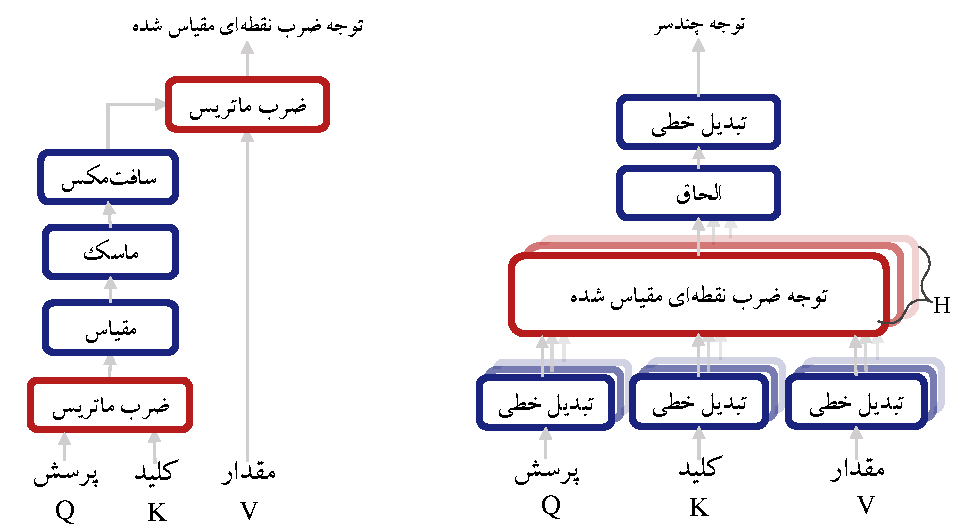
\includegraphics[scale=0.7]{Figures/attention.pdf}
	\caption[سمت چپ توجه ضرب نقطه‌ای مقیاس شده]{سمت چپ توجه ضرب نقطه‌ای مقیاس شده. سمت راست، توجه چندسر. در توجه چندسر، سرها به صورت موازی محاسبه می‌شوند.}
	\label{Fig:Attention}
\end{figure}


 معادله‌ی \ref{Eq:Attention}، نحوه‌ی محاسبه‌ی توجه ضرب نقطه‌ای مقیاس شده را نشان می‌دهد. با در نظر گرفتن $d_{k}$ به عنوان بعد بردار کلید و $d_{v}$ به عنوان بعد بردار مقدار در این معادله، کلید $K\in\mathbb{R}^{d_{k}}$، مقدار $V\in\mathbb{R}^{d_{v}}$، پرسش $Q\in\mathbb{R}^{d_{k}}$، عملیات ترانهادن\LTRfootnote{Transpose} $T$ و $.$ بیانگر ضرب ماتریس است. 
\begin{equation}
	Attention(Q, K, V) = V \times softmax(\frac{Q . K^{T}}{\sqrt{d_{k}}})
	\label{Eq:Attention}
\end{equation}
در مرجع \cite{transformer} نشان داده‌شده که برای مقادیر بزرگ $d_{k}$، مقادیر محصول نقطه‌ای بزرگ می‌شود که باعث شده تابع سافت‌مکس به نقطه‌ای برسد که گرادیان بسیار کوچکی دارد. برای مقابله با این اثر، آن‌ها با مقیاس $\frac{1}{\sqrt{d_{k}}}$ محصول نقطه‌ای را تغییر دادند؛ از این‌رو این معادله، ضرب نقطه‌ای مقیاس شده نام دارد.
\\
برای محاسبه‌ی توجه چند سر می‌توان از معادله‌ی \ref{Eq:MultiHead} استفاده کرد. در این معادله تعداد سرهای توجه $H$، و عملیات الحاق\LTRfootnote{Concatenation} با علامت $⊕$ مشخص شده است.
\begin{equation}
	\begin{array}{l}
		Attention_{h}(Q, K, V) = (Q . W_{h}^{Q}, K . W_{h}^{K}, V . W_{h}^{V}) \\
		Attention = Attention_{1} ⊕ Attention_{۲} ⊕ ... ⊕ Attention_{H} \\
		MultiHead = W^{M} . Attention
	\end{array}
	\label{Eq:MultiHead}
\end{equation}
در معادله‌ی \ref{Eq:MultiHead}، پیدا کردن روابط معنایی بین $H$ سر تقسیم شده‌اند. 
\\
درصورت تمایل برای جلوگیری از اعمال توجه بر روی برخی از موقعیت‌های درون جمله‌ی مبدا، می‌توان ماسک $M\in\mathbb{R}$ را در معادله‌ی \ref{Eq:Attention} اعمال کرد. در این صورت، معادله‌ی یاد شده به معادله‌ی \ref{Eq:MaskedAttention} تغییر می‌یابد.
\begin{equation}
	Attention_{Masked}(Q, K, V) = V \times softmax(\frac{Q . K^{T}}{\sqrt{d_{k}}}+M)
	\label{Eq:MaskedAttention}
\end{equation}
متعاقباً، مکانیزم توجه چند سر پوشیده، با معادله‌ی \ref{Eq:MaskedMultiHead} و با جابجایی مکانیزم توجه عادی با پوشیده بدست می‌آید. در این صورت، ماتریس ماسک $M_{diagonal}\in\mathbb{R}^{S\times T}$ نیز باید همراه با سایر ورودی‌ها، به تابع تغذیه شود؛ که در آن $S$ طول ترتیب مبدا و $T$ طول ترتیب مقصد است.
\begin{equation}
	\begin{array}{l}
		Attention^{h}_{masked}(Q, K, V) = (Q . W_{h}^{Q}, K . W_{h}^{K}, V . W_{h}^{V}) \\
		Attention_{masked} = Attention_{masked}^{1} ⊕ Attention_{masked}^{۲} ⊕ ... ⊕ Attention_{masked}^{H} \\
		MultiHead_{masked} = W^{M} . Attention_{masked}
	\end{array}
	\label{Eq:MaskedMultiHead}
\end{equation}
از مکانیزم توجه چند سر می‌توان برای مقاصد مختلف بهره برد. در ادامه به دو شیوه‌ی مرسوم آن و بینش پشت آن‌ها پرداخته می‌شود.
\subsubsection{توجه به خود}
زمانی که هر سه بردار کلید، مقدار و پرسش از یک جمله تولید شوند، به آن توجه به خود\LTRfootnote{Self-Attention} می‌گویند. هدف از معرفی توجه به خود، ایجاد تعبیه‌ی جدیدی برای نشانه است که در آن، تعبیه‌ی سایر نشانه‌های جمله دیده شده است. به عبارتی، به استفاده از توجه به خود، تعبیه‌ی نشانه‌ها با پیش‌زمینه‌ای که نشانه در آن استفاده شده آمیخته می‌شود.
\subsubsection{توجه متقابل}
در صورتی که کلید و مقدار از یک جمله و پرسش از جمله‌ی دیگری تولید شود، آن را توجه متقابل\LTRfootnote{Cross-Attention} می‌نامند. توجه متقابل کاربرد مهمی در وظیفه‌ی ترجمه دارد؛ چراکه با استفاده از آن، می‌توان ارتباطات معنایی میان دو جمله، در دو زبان مختلف را پیدا کرد.

\subsection{تعبیه‌ی موقعیتی}
به علت بازگشتی نبودن شبکه‌ی ترنسفورمر، باید روش دیگری برای حفظ ترتیب نشانه‌های ورودی معرفی شود. به این دلیل، در \cite{transformer} تعبیه‌ی موقعیتی را معرفی کرده‌اند. برای موقعیت نشانه‌های درون جمله، مطابق معادله \ref{Eq:PositionalEncoding} دو تابع تعریف شده است. در یک جمله، $N$ موقعیت مکانی (نشانه) و به ازاء هر نشانه، یک بردار $d_{model}$ بعدی\LTRfootnote{Dimension} وجود دارد.  معادله‌ی \ref{Eq:PositionalEncoding} برای بعدهای زوج از تابع سینوسی،‌ و برای بعدهای فرد تابع کسینوسی استفاده می‌کند. تعبیه‌ی موقعیتی، بعد یکسانی با بعد مدل $d_{model}$ دارد؛ به این منظور که بتوان تعبیه‌ی موقعیتی را با بردار تعبیه جمع کرد.
\begin{equation}
	\begin{array}{l}
		PE_(pos,2i) = Sin(\frac{pos}{10000^{\frac{2i}{d_{model}}}})\\\\
		PE_(pos,2i+1) = Cos(\frac{pos}{10000^{\frac{2i}{d_{model}}}})
	\end{array}
	\label{Eq:PositionalEncoding}
\end{equation}
در معادله‌ی بالا، موقعیت نشانه در جمله $pos$  و بعد مورد نظر آن  $i$  است. بدین ترتیب، برای بعد زوج و فرد هرکدام یک تابع وجود دارد. همچنین، طول موج‌های تولید شده یک افزایش هندسی از $2\pi$ به $2\pi . 10000$ می‌باشد. این توابع در مقایسه با توابعی که موقعیت مکانی را در طول آموزش یاد می‌گیرند، برتری دارند؛ چراکه می‌توانند در طول فرایند تست، تعبیه‌ی مکانی جملاتی با طول دیده نشده در فرایند آموزش را، در زمان تست استقرا کنند  \cite{transformer}.
\subsection{جریان داده}
در این بخش، تغییراتی که بر روی تعبیه‌ی اولیه‌ی نشانه‌ها صورت می‌گیرد تا به بردار نهائی تبدیل شود، تشریح می‌شوند. جریان داده به دو بخش زمان آموزش و زمان استنتاج\LTRfootnote{Inferrence} تقسیم می‌شوند. در ادامه، به توضیح این دو بخش پرداخته می‌شود.
\subsubsection{زمان آموزش}
به شکل \ref{Fig:Transformers} توجه کنید. در بخش رمزنگار، جمله‌ی ورودی ابتدا تبدیل به نشانه می‌شود. سپس برای این نشانه‌ها با استفاده از معادله‌ی \ref{Eq:PositionalEncoding} تعبیه‌ی موقعیتی ایجاد شده و با تعبیه‌ی اولیه نشانه‌ها جمع می‌شود. در مرحله‌ی بعد، ماتریس به دست آمده به صورت کامل و در یک مرحله وارد رمزنگار شده است؛ به این معنا که ورود ماتریس ترتیبی نیست. در بخش اول توجه به خود بر روی ماتریس ورودی ایجاد و سپس ماتریس توجه به دست آمده با ورودی جمع می‌شود. به عمل جمع کردن ماتریس توجه با ماتریس اولیه، اتصال باقی‌مانده\LTRfootnote{Residual Connection} می‌گویند \cite{residualconnection}. آخرین مرحله‌ی رمزنگار، یک شبکه‌ی تغذیه‌به‌جلو است که روی ماتریس حاصل از این شبکه نیز یک اتصال باقی‌مانده اعمال می‌شود.


در زمان آموزش، در بخش رمزگشا از شیوه‌ی اجبار معلم\LTRfootnote{Teacher Forcing} استفاده می‌شود. در این شیوه نشانه‌های هدف نیز همراه با ورودی به شبکه داده می‌شود. بدین ترتیب، به جای استفاده از خروجی شبکه برای تولید نشانه‌های احتمالی و آموزش ترتیبی مدل، فرایند آموزش را می‌توان به صورت موازی و بسیار سریع‌تر انجام داد. برای ورود نشانه‌های هدف در معماری رمزگشا، همه‌ی نشانه‌ها یک واحد به سمت راست جابجا می‌شوند؛ این کار به‌این منظور صورت می‌گیرد که شبکه بتواند در زمان استنتاج، که نشانه‌ی هدف را ندارد، با وارد کردن یک نشانه (معمولا $[BOS]$)، فرایند تولید نشانه را در رمزگشا آغاز کند. در گام نخست، ماتریس موقعیت مکانی با ماتریس تعبیه‌ی نشانه‌ها جمع شده و سپس وارد رمزگشا می‌شود. سپس عملیات توجه به خود چندسر پوشیده بر روی ماتریس تعبیه‌ی نشانه‌ها انجام و یک اتصال باقی‌مانده اعمال می‌شود. پوشیده در اینجا، به منظور استفاده از یک ماسک ماتریس مثلثی بالایی\LTRfootnote{Upper Triangular Matrix} است که از پردازش موقعیت‌های غیرمجاز توسط مکانیزم توجه جلوگیری می‌کند. این موقعیت‌های غیرمجاز در زمان آموزش، موقعیت‌های جلوتر از نشانه‌ی درحال پردازش هستند؛ چراکه کمک گرفتن از آن‌ها در زمان آموزش، برای مدل وابستگی ایجاد می‌کند، و از آن‌جا که در زمان استنتاج نشانه‌های موقعیت‌های جلوتر ناشناخته هستند، عملکرد مدل با اختلال روبرو می‌شود.
در گام دوم، کلید و مقدار از آخرین لایه‌ی رمزنگار، و پرسش از تعبیه‌ی نشانه‌ها، ایجاد و وارد واحد توجه متقابل می‌شود. در ادامه، ماتریس ایجاد شده از توجه متقابل با ماتریس تعبیه جمع، و وارد یک لایه‌ی تغذیه‌به‌جلو می‌شود. بر روی ماتریس حاصل از تغذیه‌به‌جلو نیز یک اتصال باقی‌مانده اعمال شده و بعد از یک لایه‌ی خطی و تابع سافت‌مکس، خروجی نهائی رمزگشای ترنسفورمر ایجاد می‌شود.

\subsubsection{زمان استنتاج}
تفاوت زمان استنتاج با آموزش در عدم وجود نشانه‌های هدف است؛ به همین دلیل، این تفاوت خود را در شیوه‌ی استفاده از رمزگشا نشان می‌دهد. در زمان استنتاج، رمزگشا تولید نشانه‌های خروجی را به صورت ترتیبی انجام می‌شود. بدین منظور، بعد از اتمام فرایند رمزنگاری، با دادن نشانه شروع $[BOS]$ به‌عنوان اولین نشانه به رمزگشا فرایند تولید خروجی آغاز می‌شود. سپس تمام فرایند‌های ذکرشده در زمان آموزش تکرار می‌شوند تا یک نشانه به عنوان خروجی تولید شود. خروجی تولید شده مجددا با نشانه‌ی $[BOS]$ الحاق شده و به عنوان ورودی مرحله بعد به رمزگشا تغذیه می‌شود. مراحل ذکر شده، تا رسیدن به نشانه‌ی $[EOS]$ تکرار می‌شوند.

\section{تعبیه‌ی نشانه‌ها}
برای این که جملات وارد شبکه‌ی عصبی شوند، باید ابتدا به واژه‌ها شکسته و واژه‌ها تبدیل به نشانه شوند. برای وارد کردن هر نشانه به شبکه، باید تعبیه‌ای از آن نشان وجود داشته باشد. تعبیه برداری از اعداد حقیقی است که بیانگر مفهوم آن نشانه در زبان طبیعی است. روش‌های تعبیه‌ی نشانه‌ها را می‌توان به دو گروه تقسیم نمود؛ تعبیه‌ی برداری ثابت و مدل‌های زبانی. در ادامه، این دو شیوه معرفی می‌شوند. 
\subsection{تعبیه‌ی برداری ثابت}
تعبیه برداری ثابت، نوعی از تعبیه است که در آن نمایش یک واژه یا عبارت معین از روی مجموعه‌ی متنی\LTRfootnote{Corpus} ایجاد می‌شود و در طول زمان تغییر نمی‌کند. پس از محاسبه‌ی تعبیه‌ی هر نشانه، فارغ از این ‌که نشانه در چه جمله‌ای استفاده شده باشد، تعبیه‌ی آن ثابت در نظر گرفته می‌شود. دو شیوه‌ی مطرح تعبیه‌ی برداری ثابت \lr{Word2Vec} و \lr{GloVe} هستند. در ادامه، به صورت خلاصه این دو تعبیه معرفی می‌شوند.
\subsubsection{\lr{Word2Vec}}
\lr{Word2Vec}
، مجموعه‌ای از مدل‌های شبیه به هم است که برای تعبیه‌ی واژه‌ها استفاده می‌شود. این مدل‌ها از شبکه‌ی تغذیه به جلوی کم‌عمق استفاده می‌کنند که برای بازسازی پیش‌زمینه‌ی زبانی واژه‌ها آموزش دیده‌اند. \lr{Word2Vec} مجموعه بزرگ متنی را به عنوان ورودی خود گرفته و یک فضای برداری با چند صد بعد تولید می‌کند. به هر واژه‌ی یکتا در مجموعه‌ی متنی، یک بردار متناظر در فضای برداری اختصاص داده می‌شود. \lr{Word2Vec} از دو روش برای تولید این بردارها بهره می‌برد؛ کیسه‌ی واژه‌های ممتد\LTRfootnote{Continuous bag-of-words} و اسکیپ‌گرام ممتد\LTRfootnote{Continuous Skip-Gram}. در هر دو روش،‌ یک پنجره لغزان\LTRfootnote{Sliding Window} از واژه‌های پیش‌زمینه، حول یک واژه‌ی اصلی در نظر گرفته می‌شود و به ازاء تمام واژه‌های موجود در مجموعه‌ی متنی عملیات محاسبه تکرار می‌شود. در روش کیسه‌ی واژه‌ها، مدل واژه‌ی اصلی را با استفاده از واژه‌های پیش‌زمینه‌ی موجود در پنجره حدس می‌زند. در این روش، ترتیب واژه‌های پیش‌زمینه تفاوتی ندارد. در روش اسکیپ‌گرام، مدل با گرفتن واژه‌ی اصلی، واژه‌های پیش‌زمینه‌ی آن را پیش‌بینی می‌کند. در این روش، واژه‌هایی که در پنجره ازنظر فاصله به واژه‌ی اصلی نزدیک‌تر هستند وزن بیشتری دارند. نویسندگان \lr{Word2Vec} اظهار کرده‌اند که کیسه‌ی واژه‌ها سرعت بیشتری دارد و در مقابل عملکرد اسکیپ‌گرام در مواجه با واژه‌های کمیاب بهتر است \cite{word2vec}.
\subsubsection{\lr{GloVe}}
\lr{GloVe} 
از شبکه‌ی عصبی استفاده نمی‌کند. در این شیوه‌ی تعبیه، ابتدا یک مجموعه‌ی متنی بزرگ پیمایش و ماتریس هم‌آیی واژه‌ها\LTRfootnote{Word Co-occurance Matrix} تشکیل می‌شود. سپس با این فرض که محصول نقطه‌ای بردار تعبیه‌ی دو واژه که در ماتریس هم‌آیی موجود هستند،  باید با تعداد هم‌آیی آن دو واژه رابطه داشته باشد، تعبیه‌ی واژه‌ها را در فضای برداری شکل می‌دهد \cite{glove}.
\subsection{مدل‌های زبانی}
نقص اصلی تعبیه برداری ثابت، این است که قادر به درک پیش‌زمینه‌ی مربوط به واژه نیست. این مشکل، عملکرد آن را برای پیش‌بینی دقیق معنای جمله و همچنین تولید متن محدود می‌کند. علاوه بر این، تعبیه‌های تولید شده ثابت‌اند؛ به این معنی که پس از پایان فرایند آموزش، نمی‌توان آنها را برای کاربر خاص بهینه یا با واژه‌های جدید که وارد زبان می‌شوند سازگار کرد.
یک مدل زبانی\LTRfootnote{Language Model} نسبت به زمینه کلام آگاه است؛ یعنی معنای جمله‌ای که واژه در آن‌ها آمده را درک می‌کند. این ویژگی باعث شده مدل زبانی قدرت پیش‌بینی دقیق‌تری داشته باشد. از این‌رو، یک مدل زبانی با دیدن یک جمله و در چالش حدس زدن یک جای خالی، می‌تواند واژه‌های مناسب تری را برای آن جای خالی پیشنهاد کند. در واقع، هدف اصلی مدل زبانی، محاسبه‌ی احتمال وقوع یک واژه، درون یک جمله است. به عنوان مثال، اگر عبارت "من قصد خواندن یک..." به مدل زبانی داده شود، مدل احتمال وقوع "کتاب" در ادامه‌ی این جمله را بیشتر از "خودرو" در نظر می‌گیرد. از طرف دیگر، تعبیه‌ی واژه‌ها در مدل زبانی، یک بردار ثابت نیست؛ بلکه تابعی است از سایر واژه‌هایی که در جمله حضور دارند. آموزش مدل‌های زبانی معمولا کاری هزینه‌بر و گران است. معمولا در فرایند آموزش آن‌ها، یک یا چند وظیفه بر روی حجم زیادی از داده‌های متنی تعریف می‌شود.
 \\ 
 در ادامه، ‌به معرفی دو مدل زبانی اِلمو که مبتنی بر \lr{LSTM} و بِرت که مبتنی بر ترنسفورمر است پرداخته می‌شود.
\subsubsection{المو}
\begin{figure}[!htb]
	\centering
	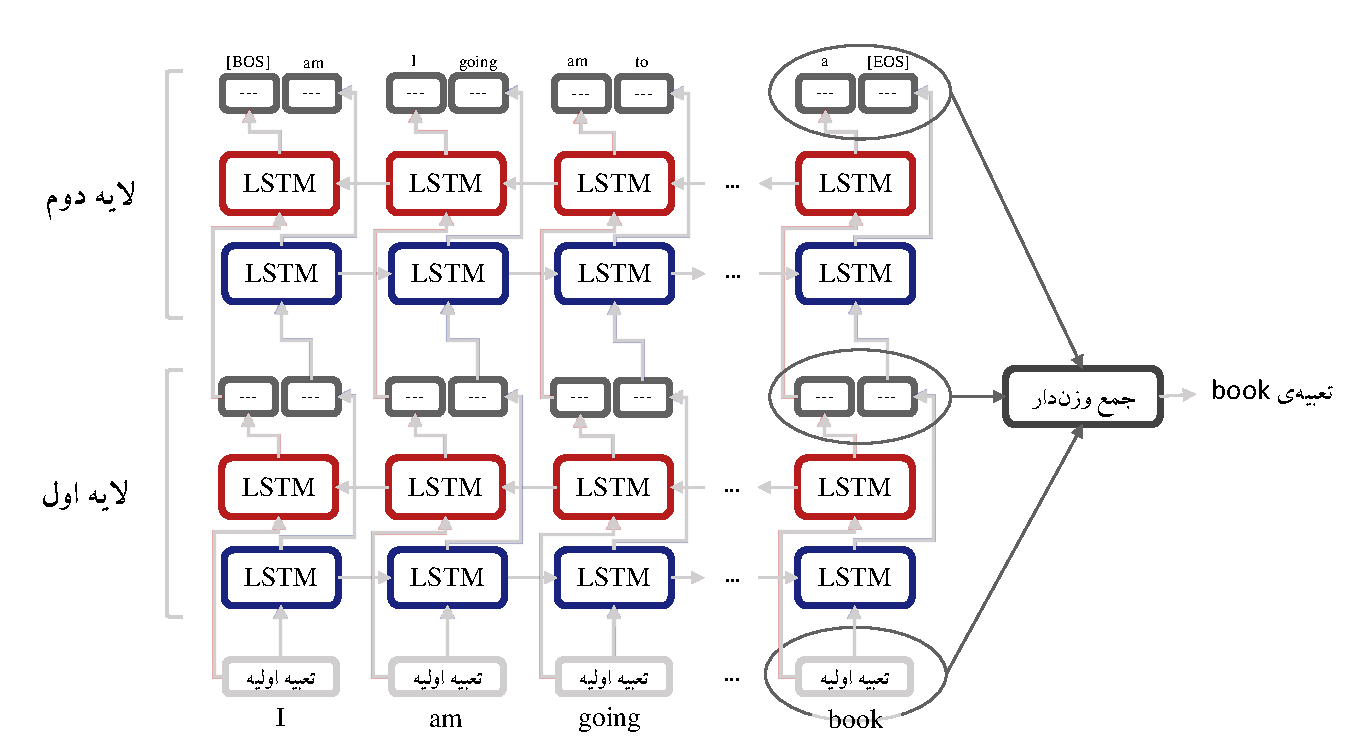
\includegraphics[scale=0.65]{Figures/elmo.pdf}
	\caption[معماری مدل زبانی المو]{معماری مدل زبانی المو. ورودی شبکه \lr{"I am going to read a book"} است. رنگ آبی برای  تعبیه‌ی چپ به راست و رنگ قرمز برای راست به چپ اختصاص دارد. برای جلوگیری از پیچیدگی شکل، اتصال باقی‌مانده در این شکل رسم نشده است.}
	\label{Fig:elmo}
\end{figure}
همانطور که گفته شد، برای ورود واژه‌ها به شبکه‌ی عصبی، باید واژه تبدیل به شناسه و شناسه تبدیل به بردار شود. در اِلمو \LTRfootnote{ELMo: Embedding From Language Models}، برای ایجاد بردار اولیه‌ی نشانه، از تعبیه‌ی الفبایی\LTRfootnote{Character Embedding} استفاده می‌شود. بدین منظور، ابتدا واژه به سطح الفبا شکسته شده، برای هر حرف الفبا یک شناسه‌ی یکتا، و برای هر شناسه یک بردار در نظر گرفته می‌شود. در مرحله‌ی بعد، مجموعه تعبیه‌ی الفبای واژه وارد شبکه‌ی کانولوشنی با اندازه هسته‌ی گوناگون می‌شود. مدل اصلی المو از هسته‌هایی با اندازه‌های ۱ تا ۷، با کانال‌های 32، 32، 64، 128، 256، 512 و 1024 استفاده می‌کند. خروجی‌های هر لایه کانولوشن پس از آن \lr{Max-Pool} شده و به هم الحاق می‌شوند تا برداری با تعداد بعد 2048 را بسازند. این خروجی به عنوان تعبیه‌ی اولیه واژه در نظر گرفته می‌شود تا مطابق شکل \ref{Fig:elmo} وارد شبکه‌ی \lr{LSTM} شود. المو در ساختار شبکه‌ی خود از \lr{LSTM} در دو جهت و به صورت دو لایه استفاده می‌کند. باید توجه داشت که ساختار شبکه با دو لایه‌ی \lr{Bi-LSTM} متفاوت است، چراکه ابتدا دو لایه متن را از چپ به راست و دو لایه را از راست به چپ پردازش می‌کند. در لایه‌ی چپ به راست،  در هر گام زمانی، وظیفه‌ی \lr{LSTM}‌ حدس زدن واژه‌ی بعدی، و در لایه‌ی راست به چپ، وظیفه‌ی آن حدس زدن واژه‌ی پیشین است. میان تعبیه‌ی اولیه و خروجی لایه‌ی اول، یک اتصال باقی‌مانده اضافه می‌شود. این عمل به مقاومت بیشتر شبکه درمقابل گرادیان محو شونده کمک می‌کند \cite{residualconnection}. در نهایت، برای تولید تعبیه‌ی پایانی، در هر لایه به صورت جداگانه، تعبیه‌ی چپ به راست با راست به چپ به یکدیگر الحاق می‌شوند. در پایان، جمع وزن‌دار میان تعبیه اولیه، خروجی الحاقی لایه‌ی اول و خروجی الحاقی لایه‌ی دوم را محاسبه می‌کنند. وزن‌های مربوط به این جمع وزن‌دار، برای هر وظیفه در پردازش زبان طبیعی متفاوت است.\\ خروجی هر لایه‌ی المو معنا و کاربرد خاص خود را دارد. خروجی لایه‌ی اول، بیشتر درمورد صرف و نحو زبان و خروجی لایه‌ی دوم، مرتبط به معنای جمله و واژه‌ها است \cite{elmo}.

\subsubsection{برت}
\begin{figure}[!htb]
	\centering
	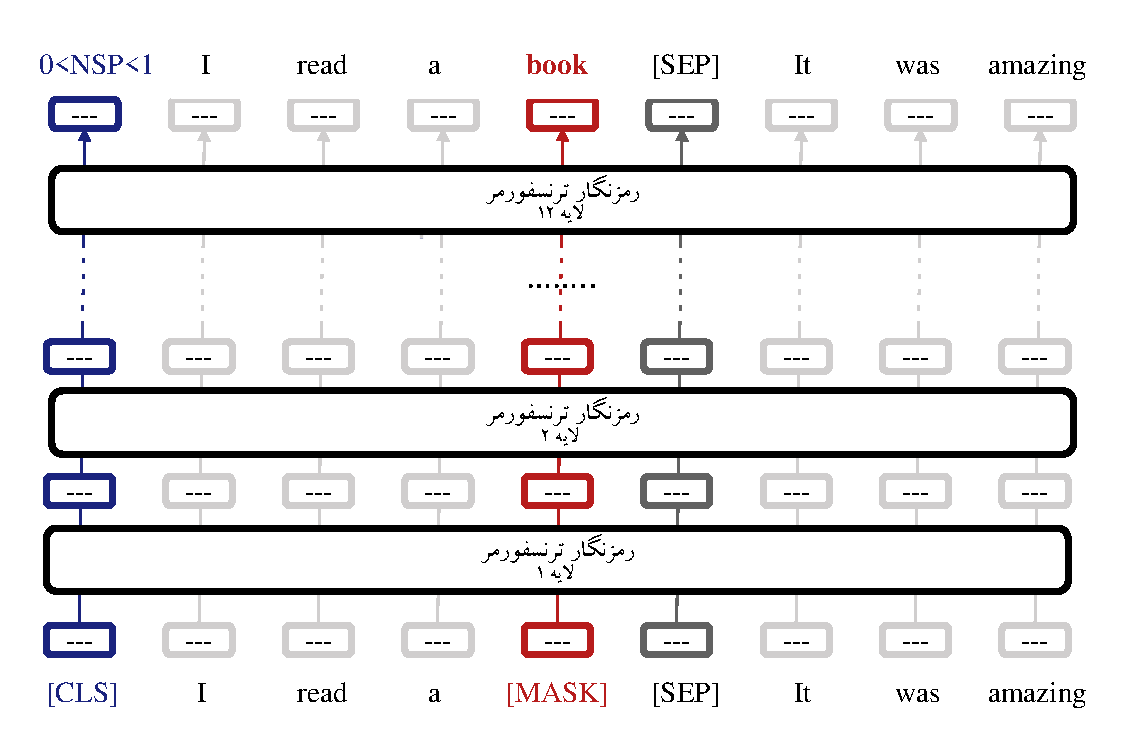
\includegraphics[scale=0.8]{Figures/bert.pdf}
	\caption[معماری مدل زبانی برت]{معماری مدل زبانی برت. ورودی شبکه دو جمله‌ی \lr{"I read a book. It was amazing"} است. واژه‌ی \lr{book} با استفاده از نشانه‌ی $[MASK]$ پوشیده شده است. این تصویر مربوط به نسخه‌ی $BERT_{base}$ می باشد.}
	\label{Fig:bert}
\end{figure}
بِرت\LTRfootnote{"Bert: Bidirectional Encoder Representations from Transformers"} 
یک مدل زبانی پیش‌آموز شده بر روی ترنسفورمرها است که برای استفاده در امور مختلف پردازش زبان طبیعی مورد استفاده قرار می‌گیرد \cite{bert}. با معرفی ترنسفورمرها \cite{transformer}، امکان ارائه یک تعبیه‌ی دوطرفه‌ی حقیقی فراهم شد. در \cite{bert} برای بهره‌گیری از قدرت ترنسفورمر، دو وظیفه‌ی خودناظر بر روی یک معماری لایه‌ای معرفی شده و ورودی‌ها به ترنسفورمر ساختارمند گردید. برای استفاده از برت، می‌توان مدل پیش‌آموز شده را دریافت کرد و با توجه به نیاز، آن را روی دیتاست مورد نظر تنظیم دقیق کرد. این شبکه در مدل پایه‌ی خود از ۱۲ لایه ترنسفورمر و در مدل بزرگ خود از ۲۴ لایه ترنسفورمر استفاده می‌کند. مدل برت در شکل \ref{Fig:bert} نمایش داده شده است.\\
  همانطور که بالا تلویحا گفته شد، برت در دو مرحله آموزش داده‌می‌شود؛ پیش‌آموزش\LTRfootnote{Pre-Training} و تنظیم دقیق\LTRfootnote{Fine-Tune}.\\
\textbf{پیش‌آموزش:}
 در این مرحله،‌ برت یاد می‌گیرد که زبان و پیش زمینه‌ی متن چیست. در مرحله پیش‌آموزش، مدل دو وظیفه‌ی متفاوت اما مرتبط را به صورت همزمان روی یک مجموعه متنی بدون برچسب یاد می‌گیرد. این دو وظیفه پیش‌بینی جمله‌ی بعد  و مدل‌سازی زبانی پوشیده هستند.\\
 الف) پیش‌بینی جمله‌ی بعد\LTRfootnote{Next Sentence Prediction (NSP)}: این وظیفه بر پایه‌ی این پیش‌فرض که دو جمله‌ی درون یک پاراگراف ازنظر معنایی به هم مرتبط هستند تعریف شده است. بر این اساس،  در وظیفه‌ی \lr{NSP}، برای دو جمله‌ی درون پاراگراف عدد ۱ و دو جمله‌ای که در یک پاراگراف نیستند عدد ۰ در نظر گرفته شده است. در این بخش، دو جمله‌ای که به مدل داده می‌شوند توسط نشانه‌ی $[SEP]$ از یکدیگر جدا شده‌اند. هدف مدل در این بخش تعیین ارتباط این دو جمله با یکدیگر است. نتیجه‌ی این تشخیص در اولین نشانه از خروجی (در شکل ‏\ref{Fig:bert} نشانه‌ی آبی رنگ) قرار دارد.\\
 ب) مدل‌سازی زبانی پوشیده\LTRfootnote{Masked Language Modeling (MLM)} : در این وظیفه مدل سعی می‌کند زمینه‌ی محتوایی متن را به صورت دوطرفه یاد بگیرد. به این منظور برخی واژه‌ها از جمله حذف شده و نشانه‌ی $[MASK]$ جای آن‌ها را می‌گیرد. سپس مدل سعی می‌کند با توجه به سایر واژه‌های موجود در جمله، جای خالی را با واژه‌ی مناسب پر کند. حذف واژه، با احتمال ۱۵ درصد روی تمام واژه‌های ورودی به جز واژه‌های کلیدی $[NSP]$ و $[SEP]$ صورت می‌گیرد.
 \\
\textbf{تنظیم دقیق:}
پس از مرحله‌ی پیش‌آموزش، برت زبان را یاد می‌گیرد اما نحوه‌ی استفاده از آن برای حل مسئله را بلد نیست. در مرحله‌ی تنظیم دقیق، مدل روش حل مسئله را آموزش می‌بیند. بدین منظور، با توجه به وظیفه‌ی مورد انتظار از مدل زبانی، نحوه‌ی آموزش مدل و ساختار رمزگشای آن مشخص می‌شود. به طور مثال می‌توان برای وظیفه‌ی پیش‌بینی احساسات، با قرار دادن یک شبکه‌ی تغذیه به جلو روی خروجی $[NSP]$ و آموزش مدل روی یک مجموعه داده‌ی پیش‌بینی احساسات، مدل را برای این وظیفه، تنظیم دقیق کرد. این کار نسبت به پیش‌آموزی، مدت زمان کمتری طول خواهد کشید؛ زیرا که شبکه به آموزش وزن‌های شبکه‌ی تغذیه به جلو که به تازگی اضافه شده‌اند می‌پردازد و بقیه‌ی پارامترهای مدل برت اندکی تغییر می‌کنند.
\section{جمع‌بندی}
در این فصل، ابتدا مفاهیم پایه‌ی این پایان‌نامه ذکر شد. سپس، مقدمه‌ای بر شبکه‌ی عصبی مطرح گردید. برای پردازش داده‌های ترتیبی، شبکه‌ی عصبی بازگشتی و \lr{LSTM} معرفی شدند. در ادامه، گفته شد که این نوع شبکه‌ها از مشکل گرادیان محو شونده رنج می‌برند. برای حل این مشکل مکانیزم توجه معرفی شد. اگرچه مکانیزم توجه مفید بود، اما اصل مسئله را حل نمی‌کرد. بنابراین، معماری ترنسفورمر معرفی گشت که از اساس ترتیبی نبوده و داده‌ها را به صورت همزمان وارد شبکه می‌کرد. همچنین، \lr{CRF} زنجیره خطی و شبکه‌ی عصبی کانولوشنی معرفی شدند. در پایان این فصل نیز، انواع تعبیه و مدل‌های زبانی معرفی گردیدند.

\chapter{کارهای پیشین}
\pagebreak
\section{‌مقدمه}
در دو فصل گذشته، مسئله‌ی درک زبان طبیعی تعریف شده و پایه‌های سازنده‌ی آن معرفی شدند. سپس مفاهیم پایه که برای فهم موضوع لازم بود ذکر شده و در ادامه، ساختار شبکه‌های عصبی گوناگون، که در حل مسئله‌ی درک زبان استفاده می‌شوند، تشریح شدند. برای بستر سازی لازم جهت معرفی مدل، لازم است کارهای پیشین معرفی شوند تا تلاش‌هایی که تا کنون برای بهبود دو وظیفه‌ی تشخیص هدف و پر کردن جای خالی صورت گرفته است، هویدا شود. بر این اساس، در فصل پیش رو، تحقیقات پیشین در این زمینه و مدل‌های ارائه شده توصیف می‌شوند. از آنجا که روش‌های ارائه شده با یکدیگر متفاوت بوده و اشتراکات اندکی دارند، دسته‌بندی آن‌ها به دسته‌های معنادار، کار دشواری است. در فصل پیش رو،  مدل‌های ارائه شده بر پایه‌ی سبک تعبیه و اساس معماری شبکه تقسیم بندی می‌شوند.


در گذشته، دو وظیفه‌ی پر کردن جای خالی و تشخیص هدف جداگانه مورد تحقیق قرار می‌گرفتند \cite{louvan2018exploring,vu2016bi}؛ اما اخیراً، نشان داده شده که آموزش مشترک این دو وظیفه، اثر مثبتی بر عملکرد هر دوی آن‌ها دارد
\cite{aligned_lstm_atten_nlu,Wang:18,goo-etal-2018-slot,zhang-2018-joint,jaech2016domain,wei2022joint}.
این امر نشان داده است که رابطه‌ای قوی بین این دو وجود دارد. آموزش همزمان این دو وظیفه به این صورت انجام می‌گیرد که برای هر دوی آن‌ها یک رمزنگار مشترک استفاده شده، اما برای هر وظیفه یک رمزگشای مستقل تعریف می‌شود. تمامی مدل‌هایی که در این زمینه‌ی درک زبان طبیعی وجود دارند، از این ساختار بهره می‌برند چراکه برتری آن ثابت شده است.
\section{مبتنی بر نمایش تعبیه برداری ثابت}

مدت‌ها است که مکانیزم توجه به همراه \lr{LSTM‌} مورد استفاده قرار می‌گیرد \cite{varghese2020bidirectional,jaech2016domain}. ترکیب این دو در وظیفه‌ی درک زبان طبیعی نیز مورد استفاده قرار گرفته و در زمان خود بهترین عملکرد را در پی داشت. از طرفی، به علت رابطه‌ی یک به یک واژه‌های ورودی به برچسب‌های خروجی، نیازی به فضای باز احتمالاتی خروجی یک \lr{LSTM‌} نبود. به عبارت دیگر، نیاز نبود طول جمله‌ی خروجی پویا باشد؛ بلکه خروجی با طول ثابت و هم اندازه با ورودی مورد انتظار است. از طرف دیگر، آگاهی از اینکه کدام موقعیت از ورودی، به خروجی مربوط است، خود یک مزیت محسوب می‌شود و باید از آن در طراحی معماری شبکه استفاده کرد \cite{xu2020end}. در طراحی مدل \lr{LSTM}‌ تراز شده، از رابطه‌ی یک به یک ورودی با خروجی بهره برده شد \cite{aligned_lstm_atten_nlu}. شکل \ref{Fig:alignedlstm} معماری مدل تراز شده را نمایش می‌دهد. در این معماری، برای رمزنگار، از یک \lr{LSTM‌} دوطرفه که به صورت مشترک در دو رمزگشا مورد بهره‌وری قرار می‌گرفت. در رمزگشای تشخیص هدف، از بردار توجه هدف، و همچنین آخرین حالت مخفی \lr{LSTM‌} رمزنگار برای کلاس بندی اهداف بهره برده شده بود. اما در رمزگشای پر کردن جای خالی، یک \lr{LSTM‌} یک طرفه تعریف شده و از رابطه‌ی یک به یک ورودی و خروجی استفاده شد. به این منظور، در هر گام زمانی، علاوه بر بردار توجه، بردار حالت مخفی مربوط به گام زمانی ورودی که متناظر با گام زمانی خروجی بود، به مدل تغذیه می‌شد. با این ترتیب از ورودی‌ها، آموزش دو وظیفه‌ی تشخیص هدف و پر کردن جای خالی، به صورت همزمان و اشتراک آن ازطریق مشترک بودن تابع خطای آن دو وظیفه بود.
\begin{figure}[!htb]
	\centering
	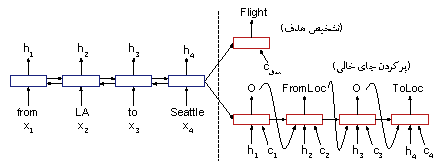
\includegraphics[scale=1.6]{Figures/alignedcnnblstm.pdf}
	\caption[ساختار مدل \lr{Aligned BLSTM}]{ساختار مدل \lr{Aligned BLSTM} \cite{aligned_lstm_atten_nlu}.}
	\label{Fig:alignedlstm}
\end{figure}


در پژوهشی دیگر، با ترکیب معماری \lr{LSTM‌} تراز شده با شبکه‌ی عصبی کانولوشنی و ساختار توالی ویژگی پنجره، نتایج بهتری به دست آمد \cite{Wang:18}. در این شبکه که آن را \lr{Aligned CNN-BLSTM} نامیدند، در بخش رمزنگار، عملیات کانولوشن با اندازه هسته‌های مختلف صورت گرفته، و نتیجه‌ی حاصل پس از ترانهاده شدن، به یکدیگر الحاق می‌شد. این ساختار را توالی ویژگی پنجره نامیدند. سپس خروجی این ساختار به یک \lr{LSTM‌} دوطرفه برای تعبیه داده می‌شد. رمزگشای پیشنهادی این مدل در هر دو وظیفه، با \lr{Aligned BLSTM} یکسان در نظر گرفته شد. شکل \ref{Fig:wang18} ساختار این شبکه را نمایش می‌دهد. این ساختار به عنوان پایه‌ی کار \lr{CTran} درنظر گرفته شد؛ از این رو در بخش ۴، شباهت زیادی میان ساختار رمزنگار پیشنهادی و این مدل خواهید دید. بخش رمزنگار این شبکه نیز کاملا با شبکه‌ی \cite{aligned_lstm_atten_nlu} یکسان بود. متعاقباً، اشتراک آموزش دو وظیفه نیز با اشتراک گذاری تابع خطا اتفاق می‌افتاد.
\begin{figure}[!htb]
	\centering
	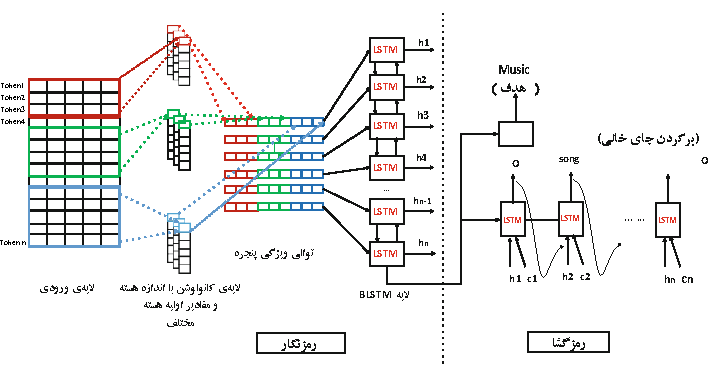
\includegraphics[scale=1.1]{Figures/cnnblstm.pdf}
	\caption[ساختار مدل \lr{Aligned CNN-BLSTM}]{ساختار مدل \lr{Aligned CNN-BLSTM} \cite{Wang:18}.}
	\label{Fig:wang18}
\end{figure}


اما در مدل \lr{Slot-Gated} \cite{goo-etal-2018-slot}، علاوه بر آموزش مشترک دو وظیفه از طریق اشتراک تابع خطا، با به اشتراک گذاری بردارهای توجه نیز اطلاعات وظیفه‌ی تشخیص هدف را در اختیار وظیفه‌ی پر کردن جای خالی گذاشتند. در معماری \lr{Slot-Gated} که در شکل \ref{Fig:slotgate} ترسیم شده، از یک شبکه‌ی \lr{LSTM‌} دوطرفه برای تعبیه‌ی جمله‌ی ورودی استفاده شد. این \lr{LSTM‌} میان هر دو وظیفه مشترکاً و به عنوان رمزنگار مدل به کار گرفته شد. سپس در رمزگشا، مکانیزم توجه \cite{attention_bahdanau} برای هر وظیفه به صورت جداگانه روی آن لایه‌ی \lr{LSTM‌} اعمال گردید. برای تولید احتمالات تشخیص هدف، آخرین خروجی \lr{LSTM‌} همراه با بردار توجه\RTLfootnote{ لازم به ذکر است که معمولا مکانیزم توجه از یک ماتریس $\mathbb{R}^{i\times j}$ تشکیل شده که در آن $i$ به عنوان طول جمله مبدا و $j$ طول جمله‌ی مقصد است؛ اما چون در تشخیص هدف تنها یک مقصد وجود دارد، یک بردار $\mathbb{R}^{i}$ تولید می‌شود.} جمع شده، سپس به یک لایه‌ی تماماً متصل تغذیه شد و با استفاده از سافت‌مکس، احتمالات خروجی برای تشخیص هدف به دست آمد.  اما برای وظیفه‌ی پر کردن جای خالی، یک دروازه‌ی جدید معرفی شد. این دروازه درواقع یک امتیاز بود که در بردار توجه جای خالی ضرب می‌شد. نتیجه‌ی ضرب، با بردار حالت مخفی برای هر مرحله از تولید برچسب جمع می‌شد و سپس بردار نهائی بدست آمده با استفاده از یک لایه‌ی تماما متصل و سافت‌مکس، احتمالات خروجی را تولید می‌کرد. به عبارتی، در معماری مدل \lr{Slot-Gated}، هیچ شبکه‌ی بازگشتی در رمزگشا استفاده نشد. امتیاز ذکر شده، از جمع وزن‌دار بردار توجه تشخیص هدف، که در بعد زمانی گسترده شده بود، با بردار توجه جای خالی بدست می‌آمد. 
\begin{figure}[!htb]
	\centering
	\includegraphics[scale=1.3]{Figures/slotgate.pdf}
	\caption[ساختار مدل \lr{Slot-Gate}]{ساختار مدل \lr{Slot-Gate} \cite{goo-etal-2018-slot}.}
	\label{Fig:slotgate}
\end{figure}


در روش \lr{Slot-Gate}، اطلاعات برچسب‌های تولید شده در تشخیص هدف مورد بهره‌وری واقع نمی‌شد؛ از این رو، ارتباطات مستقیم دوطرفه برقرار نمی‌گردید. مدل \lr{Inter-Related} \cite{e:2019} که در شکل \ref{Fig:interrelated} ترسیم شده، شبکه‌ی \lr{SF-ID} را معرفی کرد که از یک زیر شبکه‌ی پر کردن جای خالی و یک زیر شبکه‌ی تشخیص هدف ساخته می‌شد. زیر شبکه‌ی پر کردن جای خالی، اطلاعات تشخیص هدف را وارد پر کردن جای خالی کرده و در مقابل، زیر شبکه‌ی تشخیص هدف، اطلاعات برچسب‌های تولید شده را بر شبکه‌ی تشخیص هدف اعمال می‌کرد. اما برای تولید هرکدام، نیاز به داشتن دیگری است. از این رو، این مدل، مکانیزم تکرار را معرفی کرد که در آن، یک وظیفه به عنوان نقطه‌ی آغاز انتخاب می‌شد، اما فرایند انتخاب تا تعداد دفعه‌ی مشخصی تکرار می‌شد. به این ترتیب اطلاعات معنایی هر دو وظیفه می‌توانستند با یکدیگر ترکیب شوند. ازنظر ساختار شبکه‌ای، این مدل در رمزنگار خود یک \lr{LSTM‌} دوطرفه را به صورت مشترک برای دو وظیفه استفاده می‌کند. سپس در این مدل، مکانیزم توجه جداگانه برای هر وظیفه تعریف می‌شود. در رمزگشای آن، مکانیزم تکرار ابداعی قرار گرفته است. در پایان، برای تولید احتمالات هدف از لایه‌ی تماماً متصل، و برای تولید برچسب از \lr{CRF} استفاده گردیده است.
\begin{figure}[!htb]
	\centering
	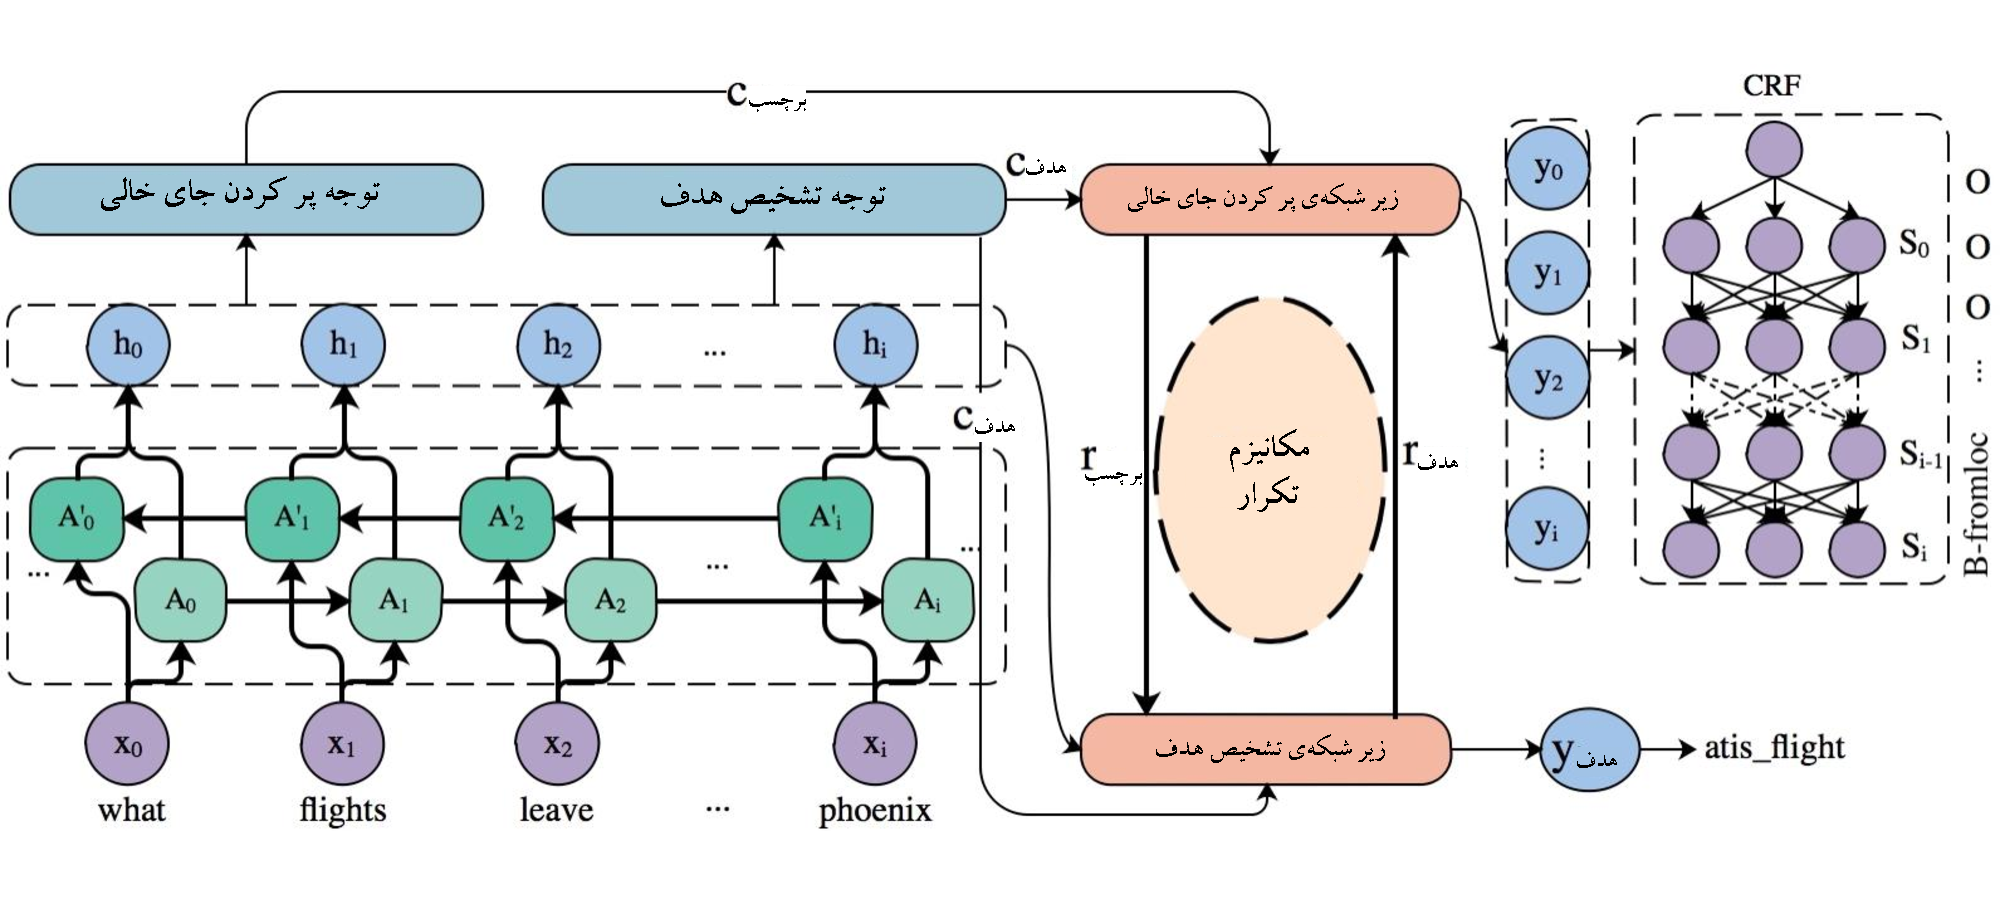
\includegraphics[scale=0.45]{Figures/interrelated.pdf}
	\caption[ساختار مدل \lr{Inter-Related}]{ساختار مدل \lr{Inter-Related} \cite{e:2019}.}
	\label{Fig:interrelated}
\end{figure}


در \lr{CharEmbed+GRU}\ \cite{Firdaus:2021} تعبیه‌ی سطح الفبا برای درک زبان طبیعی پیشنهاد شد. به این منظور، ابتدا کلمات را به الفبای سازنده شکسته، و حروف الفبای واژه را به یک \lr{LSTM‌} دوطرفه دادند تا تعبیه‌ی سطح الفبای دوطرفه ایجاد شود. در پایان، از الحاق تعبیه‌ی ایجاد شده از \lr{LSTM‌} با یک تعبیه‌ی سطح واژه مانند \lr{Word2Vec}، تعبیه‌ی نهائی واژه را ساختند. در معماری این مدل، از \lr{LSTM‌} دو طرفه برای رمزنگار و از \lr{CRF} برای رمزگشا استفاده شد.
شکل \ref{Fig:firdaus} نشان دهنده‌ی معماری \lr{CharEmbed+GRU} است که شیوه‌ی جدیدی برای ایجاد تعبیه‌ی واژه‌ها ایجاد کرد \cite{Firdaus:2021}. این مدل با قراردادن شبکه‌ی کانولوشنی بر روی الفبای کلمات و سپس عملیات \lr{Max-Pooling}، یک تعبیه‌ی سطح الفبا برای واژه ایجاد کرد. سپس تعبیه‌ی سطح الفبا را با تعبیه‌ی واژه‌ی مورد پردازش، الحاق کرد. حاصل این الحاق، به عنوان تعبیه‌ی یک واژه در نظر گرفته شد. این تعبیه برای تمام واژه‌های جمله ایجاد شده و وارد پشته‌ی \lr{LSTM} گردید تا یک تعبیه برای جمله ایجاد شود. سپس با استفاده از مکانیزم توجه \cite{attention_bahdanau} و تغذیه‌ی آن به یک لایه‌ی خطی و سافت مکس، احتمالات خروجی تشخیص هدف، پر کردن جای خالی و طبقه بندی قانون گفتگو\LTRfootnote{Dialogue Act Classification} تولید شد.
\begin{figure}[!htb]
	\centering
	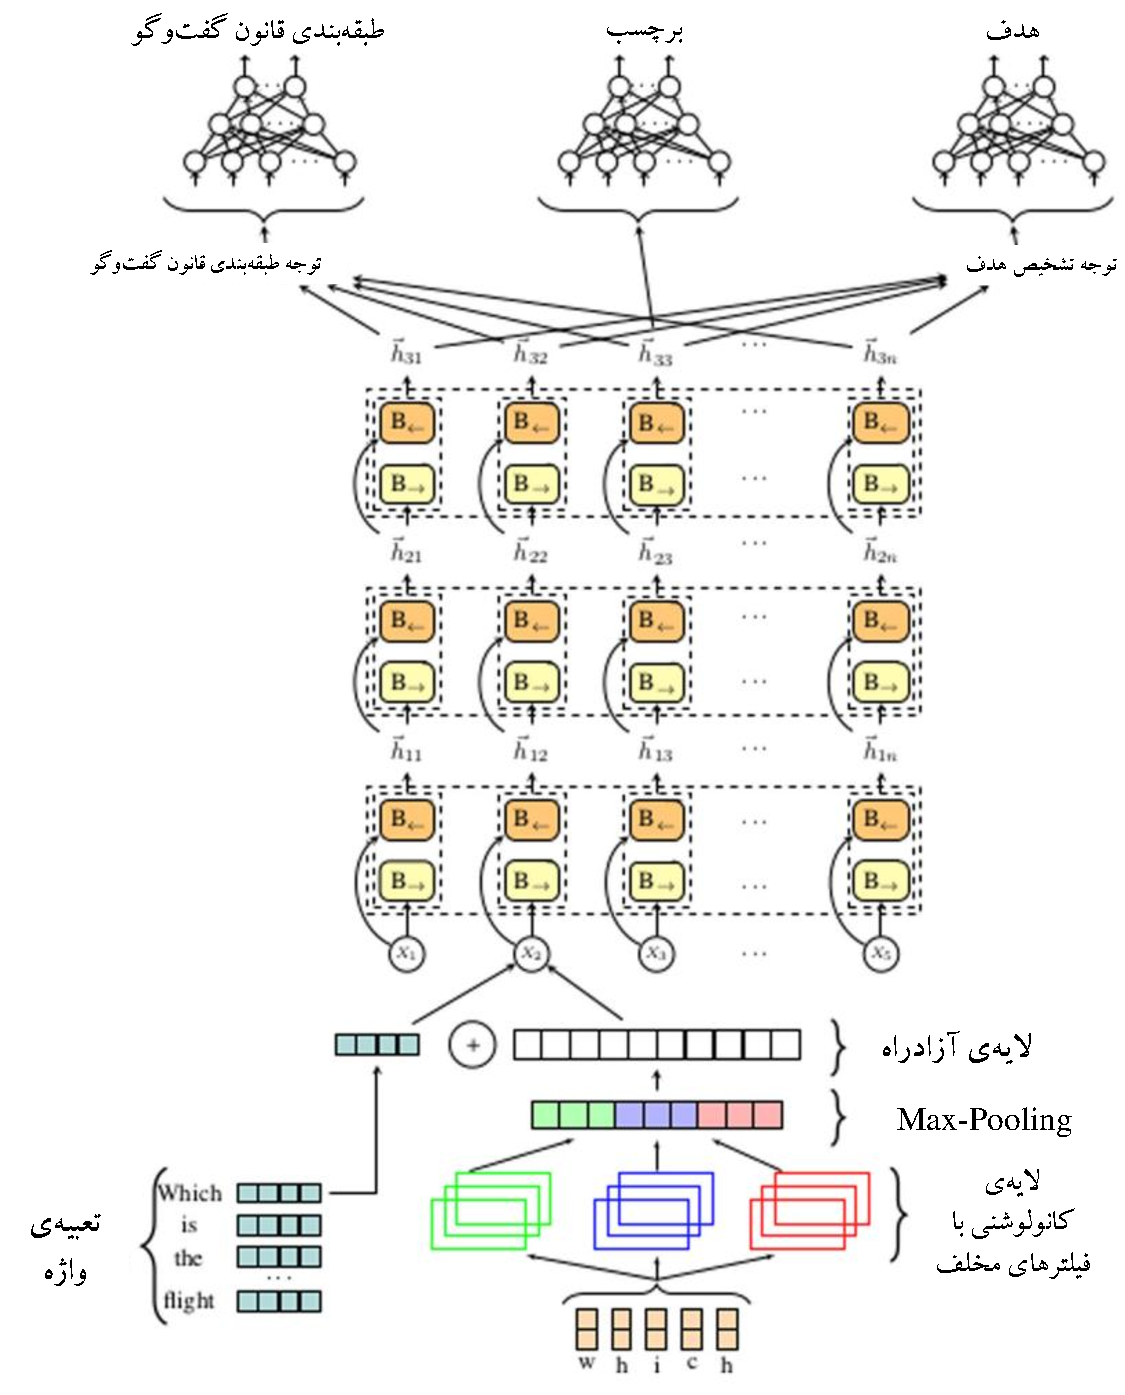
\includegraphics[scale=0.6]{Figures/firdaus2021.pdf}
	\caption[ساختار مدل پیشنهادی \lr{CharEmbed+GRU}]{ساختار مدل پیشنهادی \lr{CharEmbed+GRU} \cite{Firdaus:2021}.}
	\label{Fig:firdaus}
\end{figure}


مدل \lr{PKJL}\LTRfootnote{Prior Knowledge Joint Learning}  برای افزایش به اشتراک گذاری اطلاعات قبلی با دو وظیفه‌ی پر کردن جای خالی و تشخیص هدف معرفی شد \cite{priorknowledge}. منظور از اطلاعات قبلی، احتمال وقوع هر برچسب هدف با هر برچسب جای خالی در یک نمونه‌ی آموزشی است. در معماری پیشنهادی \lr{PKJL} که در شکل \ref{Fig:model_pkjl} ترسیم شده، مدل \lr{PKJL} با محاسبه‌ی این احتمالات و تغذیه‌ی آن به مدل خود در یک لایه‌ی ابداعی، دانش قبلی را با مدل به اشتراک گذاشت. معماری این مدل که در شکل \ref{Fig:model_pkjl}  به تصویر کشیده شده است، از یک \lr{LSTM} دو طرفه در رمزنگار و بردار احتمالات وقوع هر برچسب با هر هدف تشکیل می‌شد. یک ماژول ابداعی به نام لایه‌ی یکپارچه سازی اطلاعات بعد از رمزنگار ایجاد شد که سه ماتریس توجه برای تشخیص هدف، پر کردن جای خالی و دانش قبلی در آن تعریف می‌شدند. این سه ماتریس با یکدیگر تجمیع و تبدیل خطی شدند تا خروجی ماژول ابداعی تکمیل شود. در رمزگشای پر کردن جای خالی، یک \lr{CRF} و در رمزنگار تشخیص هدف، یک لایه‌ی خطی همراه با سافت‌مکس استفاده شد.
\begin{figure}[!htb]
	\centering
	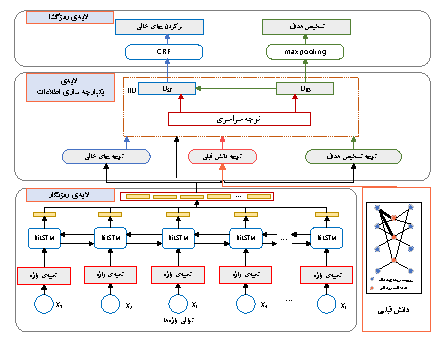
\includegraphics[scale=2]{Figures/priorknowledge.pdf}
	\caption[ساختار مدل \lr{PKJL}]{ساختار مدل \lr{PKJL} \cite{priorknowledge}.}
	\label{Fig:model_pkjl}
\end{figure}
\section{مبتنی بر مدل زبانی به عنوان رمزنگار}
طراحی مدل زبانی برت به نحوی است که استفاده از آن در وظایف مختلف پردازش زبان طبیعی بسیار ساده است. در مدل پایه که توسط \cite{chen:2019} معرفی شد، یک لایه‌ی تماماً متصل بر روی هریک از خروجی‌های برت قرار گرفت تا خروجی آن که به بعد آن، همان ابعاد تعبیه‌ی است، تبدیل به تعداد کلاس‌های برچسب‌ها و هدف‌های مجموعه داده شود. بدین ترتیب، خروجی نشانه‌ی $[CLS]$ برای مشخص کردن هدف کاربر، و نشانه‌های بخش اول ورودی به عنوان نتیجه‌ی برچسب‌زنی در نظر گرفته شد. بدین ترتیب، رمزنگار شبکه خود مدل برت و رمزگشا یک لایه‌ی تماماً متصل در نظر گرفته شد.
در معماری \cite{chen:2019}، از برت به عنوان رمزنگار استفاده شد. اما برت در درک روابط منطقی میان برچسب‌های هدف، خوب عمل نمی‌کند و این مشکل باعث می‌شود عملکرد پر کردن جای خالی شدیداً تحت تاثیر قرار گیرد \cite{Wang:2020}. از این رو، مدل \lr{SASGBC} \cite{Wang:2020} معرفی شد، که حاوی دو راهکار برای مقابله با مشکل ذکر شده  بود. این دو راهکار مکانیزم \lr{Slot-Gate} و رمزگشای \lr{CRF} بودند که هر دو مختص رمزگشای پر کردن جای خالی به کار گرفته شدند. مطابق شکل \ref{Fig:wang2020} در رمزگشای پر کردن جای خالی، نخست مکانیزم \lr{Slot-Gate} برای آمیختن هدف پیش بینی شده، با خروجی برت پیشنهاد شد. در مکانیزم \lr{Slot-Gate} پیشنهادی، خروجی تعبیه‌ی برت برای هر واژه، با بردار خروجی نشانه‌ی $[CLS]$ الحاق شده، و سپس با استفاده از یک لایه‌ی خطی بدون بایاس، ابعاد آن کاهش می‌یابد. دوم، در آخرین لایه از رمزگشا، از \lr{CRF} برای پیش‌بینی احتمالات برچسب‌ها و برای تولید برچسب‌های خروجی از الگوریتم \lr{Viterbi} استفاده شد. برای رمزگشای تشخیص هدف، صرفا یک لایه‌ی خطی همراه با سافت‌مکس، احتمالات خروجی را تعیین می‌کرد.
\begin{figure}[!htb]
	\centering
	\includegraphics[scale=0.9]{Figures/wang2020.pdf}
	\caption[ساختار مدل \lr{SASGBC}]{ساختار مدل \lr{SASGBC} \cite{Wang:2020}.}
	\label{Fig:wang2020}
\end{figure}
\section{مبتنی بر مدل زبانی به عنوان تعبیه‌گر}
از طرفی، \lr{Federated-Learning} \cite{huang:2020} رمزنگار چند نما را معرفی کرد. در این رمزنگار، یک رمزنگار برای تعبیه‌ی موقعیت، یک رمزنگار برای تعبیه‌ی اطلاعات محلی، یک تعبیه برای اطلاعات کلی (در سطح جمله) و یک رمزنگار اطلاعات توالی (سری زمانی) استفاده شد. از طرف دیگر، در برای آموزش مدل، یادگیری فدرال معرفی شد. مطابق شکل \ref{Fig:federated}، در این شیوه‌ی یادگیری، یک رمزنگار بین دو مجموعه داده‌ی \lr{ATIS} و \lr{SNIPS} مشترک بود، به این ترتیب، برای هر مجموعه داده، به صورت جدا، رمزگشای تشخیص هدف و پر کردن جای خالی تعریف شد. در نهایت، مدل باید پارامترهای رمزنگار را میان ۴ وظیفه‌ی مختلف (دو وظیفه برای هر مجموعه داده) به اشتراک می‌گذاشت. نکته‌ی پایانی در مورد مدل \lr{Federated-Learning} ، استفاده‌ی آن از برت به عنوان تعبیه‌ی کلمات بود.
\begin{figure}[!htb]
	\centering
	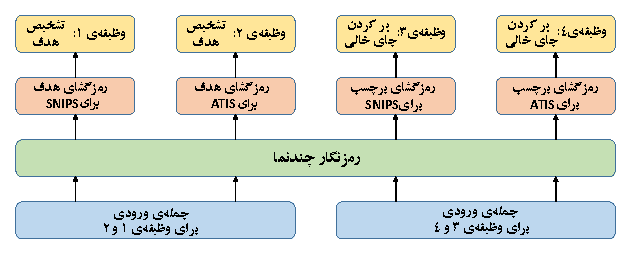
\includegraphics[scale=1.4]{Figures/federated.pdf}
	\caption[ساختار مدل \lr{Federated-Learning}]{ساختار مدل \lr{Federated-Learning} \cite{huang:2020}.}
	\label{Fig:federated}
\end{figure}


معماری \lr{Co-Interactive Transformer} \cite{Qin:2021} برای ادغام پیش زمینه‌ی تشخیص هدف و پر کردن جای خالی در یکدیگر معرفی شد و از مکانیزم توجه چند سر \cite{transformer} استفاده کرد. در \lr{Co-Interactive} به جای معماری رمزنگار - رمزگشا، معماری رمزنگار - ماژول تعاملی - رمزگشا معرفی شد. در رمزنگار، از یک \lr{LSTM‌} دوطرفه استفاده شد. سپس با استفاده از مکانیزم توجه \cite{attention_bahdanau}، برای تشخیص هدف و پر کردن جای خالی، به صورت جداگانه ماتریس توجه به دست آمد. در ماژول تعاملی پیشنهادی، از مکانیزم توجه چند سر \cite{transformer} استفاده شد؛ به این نحو که به ازای هر وظیفه‌ی، یک تبدیل خطی از ماتریس توجه آن وظیفه برای کلید، مقدار و پرسش ایجاد شد. سپس، ماتریس توجه برای هر وظیفه، با استفاده از کلید و مقدار همان وظیفه و پرسش وظیفه‌ی دیگر، محاسبه شد. بدین ترتیب در این ماژول، اطلاعات ماتریس توجه مربوط به هر دو وظیفه با یکدیگر ترکیب شد. در گام بعدی، مانند معماری ترنسفورمر، ماتریس ورودی با خروجی مکانیزم توجه توصیفی برای هر وظیفه، جمع و نرمالایز شد. در لایه‌ی تغذیه به جلو‌ی ماژول تعاملی، خروجی هرکدام از داده‌های نرمالایز شده مربوط به وظایف با یکدیگر الحاق شده و به یک لایه‌ی تغذیه به جلو داده می‌شود. حاصل خروجی این لایه‌ی تغذیه به جلو با خروجی لایه‌ی توجه تعاملی، جمع و نرمالایز شد. در پایان، برای رمزگشای پر کردن جای خالی از \lr{CRF}، و برای رمزگشای تشخیص هدف از \lr{Max-Pooling} استفاده شد.
\begin{figure}[!htb]
	\centering
	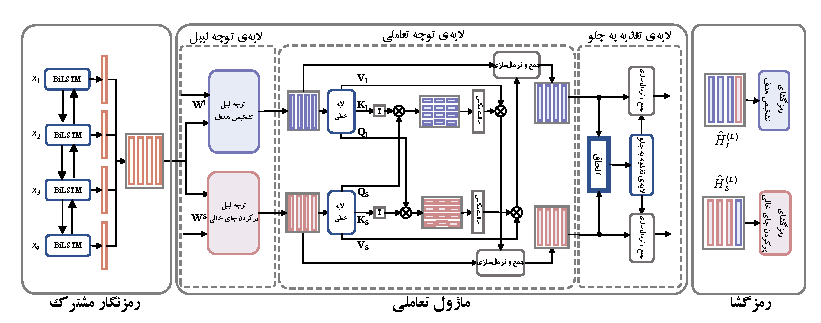
\includegraphics[scale=1.12]{Figures/cointeractive.pdf}
	\caption[ساختار مدل \lr{Co-Interactive Transformer}]{ساختار مدل \lr{Co-Interactive Transformer} \cite{Qin:2021}.}
	\label{Fig:cointeractive}
\end{figure}


در تلاشی دیگر برای ادغام بهینه‌ی دو وظیفه‌ی تشخیص هدف و پر کردن جای خالی، \lr{AISE} \cite{yang:2021} معرفی شد. معماری \lr{AISE}\LTRfootnote{Attending to Intent and Slots Explicitly} که در شکل \ref{Fig:aise} به تصویر کشیده شده، متشکل از یک رمزنگار مشترک، یک رمزنگار تشخیص هدف و مکانیزم پیشنهادی توجه چند سر پوشیده‌ی آگاه از موقعیت بود. مدل \lr{AISE} بر مبنای \lr{LSTM‌} و مکانیزم توجه چند سر بنا شد. در رمزگشای تشخیص هدف، از مکانیزم ادغام توجه چند سر استفاده کردند. ادغام توجه چند سر، نوعی از ادغام میانگین است که در آن وزن‌ها در میانگین گیری قابل تنظیم است. در این مکانیزم، کلید و مقدار از تعبیه‌ی رمزنگار و پرسش یک بردار، با مقادیر اولیه تصادفی و قابل آموزش است. خروجی این مکانیزم نیز، یک بردار با بعد تعبیه‌ی ورودی می‌باشد. در \lr{AISE}، برای رمزگشای پر کردن جای خالی، مکانیزم چند سر پوشیده‌ی آگاه از موقعیت معرفی شد. در مکانیزم پیشنهادی، از توجه چند سر پوشیده و برای تعبیه‌سازی ورودی نیز از تعبیه‌ی نسبی \cite{relative_positioning_transformer} استفاده شد. با توجه به اینکه خروجی‌های رمزگشای \lr{AISE} به صورت ترتیبی تولید شدند، در مکانیزم چند سر پوشیده، از تعبیه‌ی رمزنگار در موقعیت مربوط به نشانه‌ی درحال تولید به عنوان بردار پرسش استفاده می‌شد. همچنین از الحاق بردار زمینه‌ی تشخیص هدف و ماتریس تعبیه‌ی ابتدایی جمله به عنوان کلید و مقدار استفاده شد. در پایان، برچسب تولیدی در هر موقعیت، با استفاده از الحاق و سافت‌مکس بردار خروجی توجه چند سر پوشیده با بردار تعبیه‌ی مربوط به آن نشانه به دست آمد.
\begin{figure}[!htb]
	\centering
	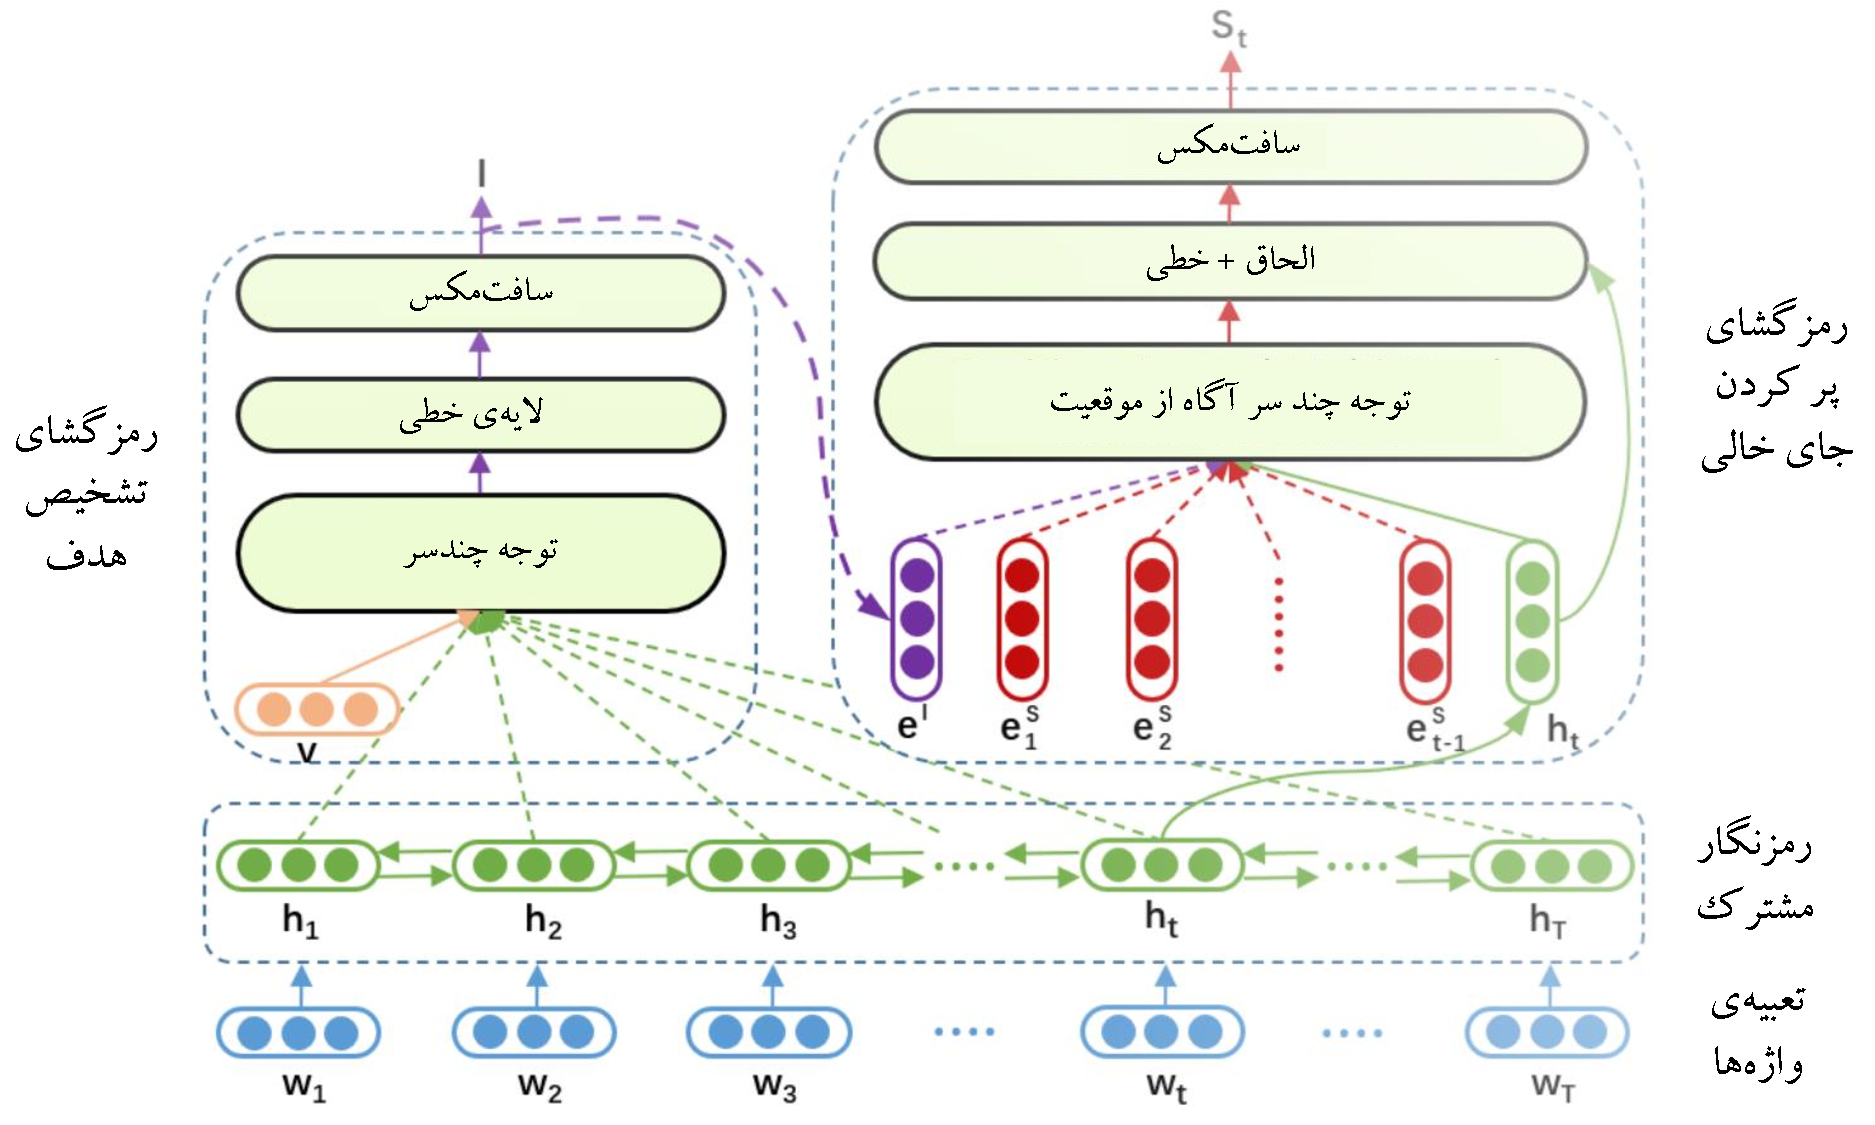
\includegraphics[scale=0.5]{Figures/aise.pdf}
	\caption[ساختار مدل \lr{AISE}]{ساختار مدل \lr{AISE} \cite{yang:2021}.}
	\label{Fig:aise}
\end{figure}


همچنین مدل پیشنهادی در \cite{Siddhant:2019} از المو به عنوان تعبیه‌ی اولیه، \lr{LSTM‌} دو طرفه به عنوان رمزنگار و \lr{CRF} به عنوان رمزگشا استفاده کرد. در این مقاله، به ارائه یک مدل زبانی تنظیم شده برای وظیفه‌ی برچسب زنی پرداخته شد و چند استراتژی برای سبک کردن مدل زبانی المو ارائه شد.
\section{جمع‌بندی}
در این فصل، انواع مدل‌های پیشین برای وظیفه‌ی درک زبان طبیعی ارائه شدند. از میان مدل‌های مبتنی بر تعبیه ثابت، \lr{Aligned LSTM} \cite{aligned_lstm_atten_nlu} با مکانیزم توجه، نخستین مدلی بود که اهمیت تراز بودن ورودی و خروجی را بیان کرد. سپس، مدل \lr{Aligned CNN-BLSTM} \cite{Wang:18} از ساختار لایه‌ی کانولوشنی-توالی ویژگی پنجره برای تعبیه‌ی ورودی خود استفاده کرد. مدل \lr{Slot-Gate} \cite{goo-etal-2018-slot} آموزش ضمنی دو وظیفه با یک رمزنگار مشترک را کافی نمی‌دانست؛ از این رو مکانیزمی برای کارگزاری هدف تشخیص داده شده در ورودی رمزگشای پر کردن جای خالی ارائه کرد. مدل \lr{Inter-Related} \cite{e:2019} این مکانیزم را یک طرفه دانست و مکانیزمی دو طرفه برای دخالت هر دو رمزگشا در یکدیگر ارائه کرد. همچنین، مدل \lr{PKJL} \cite{priorknowledge} برای دخالت دانش پیش‌زمینه در رمزگشا و مدل \lr{CharEmbed+GRU}‌ \cite{Firdaus:2021} برای ارائه یک تعبیه‌ی جدید معرفی گشتند. از طرف دیگر، در میان کارهایی که از مدل زبانی به عنوان رمزنگار استفاده کردند، برت و \lr{CRF} \cite{chen:2019} برای تولید برچسب استفاده شد. همچنین، \lr{SASGBC} \cite{Wang:2020} مکانیزم \lr{Slot-Gate} را پس از برت استفاده کرد. برخی از معماری‌های ارائه شده نیز مدل زبانی را به عنوان تعبیه‌ی کلمات استفاده کردند. در این میان، \lr{Federated Learning} \cite{huang:2020} رمزنگار چند نما و همچنین آموزش همزمان رمزنگار بر روی چند مجموعه داده را معرفی کرد. معماری \lr{Co-Interactive Transformer} \cite{Qin:2021} روشی جدید برای ادغام پیش زمینه‌ی تشخیص هدف و پر کردن جای خالی با استفاده از به اشتراک گذاری کلید و مقدار معرفی کرد. در پایان نیز، مدل \lr{AISE} \cite{yang:2021} شیوه‌ای جدید برای تولید برچسب، با استفاده از توجه چند سر آگاه از موقعیت ارائه کرد.






\chapter{مدل پیشنهادی}
\pagebreak
\section{مقدمه}
در فصل گذشته، روش‌های مطرح درک زبان طبیعی  معرفی شده و به بررسی هرکدام از روش‌ها پرداخته شد. از میان این روش‌ها، مدل \lr{Aligned CNN-BLSTM} \cite{Wang:18} به عنوان نقطه‌ی شروع این پایان نامه انتخاب شد. علت این امر، عملکرد مناسب این مدل در وظیفه‌ی پر کردن جای خالی، با وجود عدم استفاده از مدل‌های زبانی بود. به نظر می‌رسید مدل مذکور، با ایجاد تغییرات و استفاده از معماری‌های امروزی، بتواند عملکرد بهتری از خود نشان دهد. از طرف دیگر، \cite{Wang:18} در معماری خود از شیوه‌ی تراز کردن رمزگشا برای تولید تگ استفاده می‌کرد. شیوه‌ی تراز کردن \lr{LSTM} با رمزگشای ترنسفورمر سازگار نیست؛ از این رو جای خالی یک رمزگشای ترنسفورمر تراز شده نیز حس می‌شد. به همین دلیل، در این پایان‌نامه، مدل \lr{CTran}\LTRfootnote{\textbf{C}NN-\textbf{Tran}sformer} با تکیه بر شبکه‌ی کانولوشنی و ترنسفورمرها طراحی شد. در ادامه، ابتدا ساختار کلی معماری پیشنهادی را نمایش داده و سپس به تفصیل، اجزای سازنده‌ی آن توصیف می‌شود.

\section{طرح مدل}
معماری \lr{CTran} از یک رمزنگار مشترک، یک رمزگشای تشخیص هدف و یک رمزگشای پر کردن جای خالی تشکیل می‌شود. ابتدا جمله‌ی کاربر به عنوان ورودی، وارد رمزنگار شده و تعبیه‌ی میانی تولید می‌شود. این تعبیه‌ی میانی، به صورت همزمان وارد دو رمزگشا می‌شود. وظیفه‌ی رمزگشا در معماری، تولید خروجی‌های مدل است. هر رمزگشا، معماری منحصر به فردی دارد که برای وظیفه‌ی مورد نظرش طراحی گردیده است. برای اصلاح وزن‌های شبکه و آموزش مدل،خروجی‌های تولید شده با خروجی‌های مورد انتظار مقایسه شده و خطا محاسبه می‌شود. در مرحله‌ی بعد، وزن‌های هر رمزگشا به صورت جداگانه اصلاح می‌شود؛ اما از آن جا که رمزنگار بین دو وظیفه مشترک است، خطاهای هر دو وظیفه روی وزن‌های آن اثر می‌گذارند. در این بخش، ابتدا به معماری رمزنگار، سپس معماری رمزگشای تشخیص هدف و در پایان به معماری رمزگشای پر کردن جای خالی پرداخته می‌شود.
\begin{figure}[!htb]
	\centering
	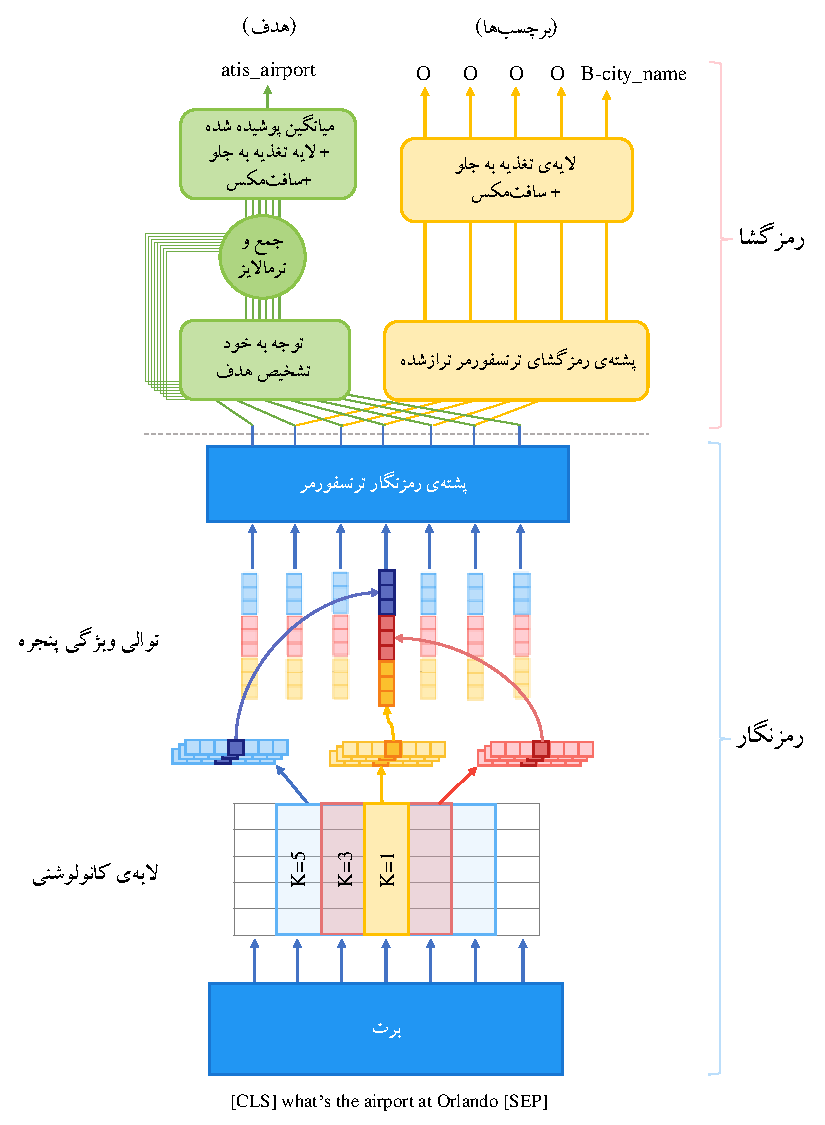
\includegraphics[scale=1]{Figures/modelarchitecture.pdf}
	\caption[معماری مدل پیشنهادی \lr{CTran}]{معماری مدل پیشنهادی \lr{CTran}. دو نشانه‌ی اضافه‌شده $[CLS]$ و $[SEP]$ از نشانه‌های ساختاری برت هستند. در زمان ورود تعبیه‌ی ایجاد شده به رمزگشای پر کردن جای خالی، تعبیه‌های متناظر با این دو نشانه، دور ریخته می‌شوند.}
	\label{Fig:architecture}
\end{figure}
\section{رمزنگار}
همانطور که گفته شد، \lr{CTran} از رمزنگار مشترک بهره می‌برد. رمزنگار شامل یک مدل زبانی پیش‌آموز شده، شبکه‌ی عصبی کانولوشنی، ساختار توالی ویژگی پنجره و پشته‌ی رمزنگار ترنسفورمر می‌شود. مطابق شکل \ref{Fig:architecture} در گام نخست، نشانه‌ها وارد مدل زبانی می‌شود تا تعبیه‌ای آگاه از پیش زمینه به دست آید. این تعبیه، به عنوان نقطه‌ی شروعی برای رمزنگار است. در گام بعد، این تعبیه‌ها وارد لایه‌ی کانولوشنی با اندازه هسته‌های مختلف می‌شود. استفاده از عملیات \lr{Max-Pooling} بعد از کانولوشن رایج است، اما با هدف حفظ توالی واژه‌ها، از ساختاری به نام توالی ویژگی پنجره استفاده شده است. در این ساختار، تمام بردارهای تولید شده برای یک واژه، ترانهاده شده و به یکدیگر الحاق می‌شوند. آخرین بخش رمزنگار، پشته‌ی رمزنگار ترنسفورمر است، که برای ایجاد تعبیه‌ی جدیدی که حاصل توالی ویژگی پنجره است، استفاده شده است. در ادامه، اجزاء سازنده‌ی رمزنگار تشریح می‌شوند.
\subsection{مدل زبانی پیش‌آموز شده}
اثبات شده که مدل‌های زبانی پیش‌آموز شده مانند برت و المو، برای بهبود عملکرد وظیفه‌های پردازش زبان طبیعی مفید هستند \cite{ethayarajh-2019-contextual}. در این پژوهش، هر دو مدل زبانی یاد شده در معماری پیشنهادی استفاده شده و نتایج آن‌ها مقایسه شدند.
ورودی برت جمعی تعبیه‌ی نشانه‌های \lr{WordPiece} \cite{wordpiece}، تعبیه‌ی موقعیتی و تعبیه‌ی بخش\LTRfootnote{Segment Embedding} می‌باشد. تعبیه‌ی بخش در مورد استفاده‌ی تک جمله‌ای معنا ندارد، چرا که تنها یک جمله وارد برت می‌شود. برای نشانه‌های ورودی $X=\left [x_{1},x_{2},x_{3},...,x_{L}\right ]$،  برت یک تعبیه‌ی آگاه به زمینه $H=\left [h_{1},h_{2},h_{3},...,h_{L}\right ]$ برای مدل فراهم می‌کند. توجه داشته باشید که نشانه ساز\LTRfootnote{Tokenizer} \lr{WordPiece} ممکن است واژه‌ها را به چند نشانه بشکند. این امر رابطه‌ی یک به یک واژه‌ی ورودی با برچسب را برهم میزند. همچنین، برچسب زدن نشانه‌های شکسته شده بیهوده است؛ چراکه همه‌ی آن‌ها به یک واژه تعلق داشته و برچسب یکسانی دارند. علاوه بر این، \lr{WordPiece} واژه‌های دارای علائم را نیز به چند نشانه می‌شکند. در روش پیشنهادی، این مشکل با حذف علائم درون واژه‌ها برطرف گردید. برای جلوگیری از حذف واژه‌هایی که فقط دارای علائم بوده و فاقد عدد و الفبا هستند، استثنا ایجاد گردید و علائم درون این واژه‌ها حذف نشدند. همچنین، همانطور که در بخش دو گفته شد، ورودی برت دارای نشانه‌های خاص است. این نشانه‌ها برای وظیفه‌ی پر کردن جای خالی در نظر گرفته نمی‌شوند.
	\\
برخلاف برت، نشانه ساز زبانی المو واژه‌ها را نمی‌شکند. از این رو ترتیب ورودی و خروجی یکسان است. در معماری پیشنهادی، از تعبیه‌های لایه‌ی آخر المو که حاوی تعبیه معنایی واژه‌ها است بهره برده شد.
\subsection{شبکه‌ی کانولوشنی}
در \cite{zhou:15clstm,Wang:18}، شبکه‌ی عصبی کانولوشنی برای پوشش کاستی‌های \lr{LSTM} استفاده شد. از آنجا که ترنسفورمر کاستی‌های یاد شده را برطرف کرده است، ممکن است استفاده از شبکه‌ی کانولوشنی بیهوده به نظر برسد. اما از طرفی، اثر استفاده از شبکه‌ی کانولوشنی در کنار ترنسفورمر برای وظیفه‌ی درک زبان طبیعی بررسی نشده است. در این پژوهش، از شبکه‌ی کانولوشنی، برای استخراج اطلاعات معنایی و همچنین ادغام آن‌ها در پنجره‌های مشخص استفاده شده است. این ویژگی از آن سو مورد توجه این پژوهش قرار گرفت، که ترنسفورمر، ذاتاً تفاوتی میان واژه‌های نزدیک به واژه‌ی اصلی و واژه‌های دورتر قائل نیست. این در حالی است که فرض اولیه‌ی مدل‌هایی مانند \lr{n-gram} \cite{ngram}، \lr{GloVe} و \lr{Word2Vec}، بر نقش کلیدی واژه‌های مجاور است. به همین علت، در معماری پیشنهادی، از چند لایه‌ی کانولوشنی، با اندازه هسته و مقادیر اولیه‌ی متفاوت استفاده شده، تا تعبیه‌ی واژه‌های همسایه با واژه‌ی مورد نظر آمیخته شود. این امر به منظور تاکید اثرگذاری واژه‌های همسایه بر معنای واژه‌ی فعلی است؛ امری که در \lr{LSTM} برای پوشش نقش دروازه‌ی ورودی صورت می‌گرفت.\\
اگر $d_{lm}$ نمایانگر بُعد تعبیه و جمله ورودی حاوی $L$ نشانه باشد، تعبیه‌ی جمله‌ی ورودی به صورت $h\in\mathbb{R}^{L\times d_{lm}}$ تعریف می‌شود و بردار تعبیه برای $i$-امین نشانه با $h_{i}\in \mathbb{R}^{d_{lm}}$ نشان داده می‌شود. اجازه دهید $k$ اندازه‌ی هسته باشد و $f\in\mathbb{R}^{k\times d_{lm}}$ یک هسته را نشان دهد. با این فرضیات، برای هر موقعیت $i$ در جمله، یک پنجره
 $w_{i}\in\mathbb{R}^{k\times d_{lm}}$
  وجود دارد که حاوی $k$ بردار نشانه بوده و به صورت $w_{i}=\left[h_{i},h_{i+1},h_{i+2}،\cdot،h_{i+k-1}\right]$ تعریف می‌شود. در صورتی که 
$\odot$
 ضرب عنصری، $b\in\mathbb{R}$ پارامتر بایاس و $A$ یک تابع فعال ساز باشد، عملیات کانولوشن $c_{i}$ برای هر پنجره $w_{i}$ توسط معادله‌ی \ref{Eq:Cnnoperation} محاسبه می‌شود. مدنظر داشته باشید که بعد از ضرب عنصری، تمام مقادیر ماتریس با یکدیگر جمع می‌شوند تا یک عدد به دست آید.
 \begin{equation}
 	c_{i}=A\left(w_{i}\odot f+b\right)
 	\label{Eq:Cnnoperation} 
 \end{equation}
این عملیات به ازاء $0<i<k$، یعنی تمام موقعیت‌های درون جمله انجام می شود. بر همین اساس، خروجی کانولوشن $f$ بر روی $x$ با $C=\left[c_{1},c_{2},c_{3},...,c_{i},...,c_{L}\right]$ نمایش داده می‌شود. لازم به ذکر است که در \lr{CTran} از پد صفر استفاده گردید؛ به همین دلیل اندازه‌ی ورودی و خروجی لایه‌ی کانولوشنی همواره برابر است. پد صفر برای حفظ برابر طول جمله‌ی خروجی با ورودی استفاده شد؛ چرا که در گام بعد، این بردارها با یکدیگر الحاق می‌شوند. از این رو، برابر بودن اندازه‌ی ورودی و خروجی اهمیت بالایی دارد.
\subsection{توالی ویژگی پنجره}
استفاده از عملیات \lr{Pooling} بعد از لایه‌ی کانولوشنی مرسوم است، اما نمونه بَرداری ناپیوسته\LTRfootnote{Discontinuous Sampling} باعث از دست رفتن برخی از اطلاعات می‌شود، و در نتیجه، این عملیات‌ها باعث از بین رفتن اطلاعات ترتیبی، در توالی داده‌ها می‌شود \cite{Wang:18}. در این پژوهش، به منظور حفظ ترتیب اصلی نشانه‌ها، از توالی ویژگی پنجره استفاده شد. در این ساختار، تعبیه‌ی نشانه‌ها با اندازه‌ی هسته‌ی مختلف و تعداد کانال خروجی مختلف، به یکدیگر الحاق می‌شوند تا یک بردار تعبیه برای آن نشانه تشکیل دهند.\\
فرض کنید $d_{conv}$ تعداد کل هسته‌ها، با اندازه‌ی هسته و مقادیر اولیه‌ی متفاوت برای هسته و $j$ بیانگر موقعیت $j$-امین فیلتر باشد. با در نظر گرفتن $\oplus$ به عنوان عملیات الحاق، $r_{i}\in\mathbb{R}^{d_{conv}}$ تعریف شده در معادله \ref{cnnfinal}، نمایش نهائی واژه‌ی $i$-ام را تعریف می‌کند و $C_{i}^{j}$ نشان دهنده $i$-امین عنصر فیلتر $j$-ام است.
\begin{equation}
	\label{cnnfinal}
	r_{i}=C_{i}^{1} \oplus C_{i}^{2} \oplus C_{i}^{3} \oplus ... \oplus C_{i}^{j} \oplus ... \oplus C_{i}^{d_{conv}}
\end{equation}
بنابراین $r_{i}$ تمام مقادیر کانولوشن متعلق به موقعیت $i$ را برای همه هسته‌ها به هم الحاق می‌کند.
این عملیات برای همه موقعیت‌ها انجام می‌شود تا زمانی که این نمایش برای همه واژه‌های ورودی تولید شود. خروجی ساختار توالی ویژگی پنجره، به شکل $R=\{r_{1},r_{2},r_{3},\cdots,r_{L}\}$ می‌باشد. در مرحله‌ی آخر، خروجی این ساختار به پشته‌ی رمزنگار ترنسفورمر تغذیه می‌شود تا نمایش نهائی تولید گردد.
\subsection{پشته‌ی رمزنگار ترنسفورمر}
امکان دسترسی مستقیم به تمام موقعیت‌های درون جمله، به رمزنگار ترنسفورمر کمک می‌کند تا بر از دست دادن اطلاعات غلبه کند. برتری آشکار ترنسفورمر باعث شد که از این شبکه، به جای  \lr{LSTM} استفاده شود.
پشته‌ی رمزگشای ترنسفورمر، همانطور که در شکل \ref{Fig:bert} نشان داده شد، از چندین لایه تشکیل شده است که در آن، خروجی هر لایه به عنوان ورودی لایه بعدی استفاده می‌شود. با توجه به ساختار رمزنگار ترنسفورمر، ابعاد خروجی آن برابر با ورودی است؛ یعنی خروجی این لایه برابر با $H\in\mathbb{R}^{L\times d_{conv}}$ می‌باشد.

\section{رمزگشا}
ماتریس ایجاد شده در رمزنگار $H$، که در این پایان‌نامه حافظه نامیده شده، به صورت همزمان به دو رمزگشا تغذیه می‌شود. این ماتریس به عنوان نقطه‌ی آغاز شبکه‌های رمزگشا است. هرکدام از این دو رمزگشا، تغییرات متناسب با ساختار احتمالات خروجی را، بر روی ماتریس ایجاد می‌کنند. در ادامه، شبکه‌های پیشنهادی برای رمزگشای تشخیص هدف و رمزگشای پر کردن جای خالی معرفی می‌شوند.
\subsection{رمزگشای تشخیص هدف}
همانطور که در شکل \ref{Fig:architecture} ترسیم شده، رمزگشای تشخیص هدف از یک لایه‌ی توجه به خود با اتصال باقی‌مانده و لایه‌ی نرمال سازی تشکیل شده است. معادله‌ی \ref{Eq:intent_attention} بیانگر عملیات یاد شده است. 
\begin{equation}
	D_{intent} = H + LayerNorm(  MultiHead(H)  )
	\label{Eq:intent_attention}
\end{equation}
 در ادامه، یک لایه‌ی تغذیه به جلو و سافت‌مکس برای محاسبه‌ی احتمالات خروجی مورد بهره‌وری قرار گرفته است. بر این اساس، ابتدا میانگین تعبیه‌ی نشانه‌های درون جمله محاسبه می‌شود. در محاسبه‌ی این میانگین، تعبیه‌ی نشانه‌هایی که برای پد کردن جمله اضافه شده‌اند نادیده گرفته می‌شود؛ بدین جهت، این میانگین، پوشیده نامیده شده است. بعد از اعمال میانگین پوشیده، طول جمله $L$ در خروجی مرحله قبل $D_{intent}\in\mathbb{R}^{L\times V}$، فرو می‌ریزد و این ماتریس تبدیل به یک بردار $D_{intent}^{\prime}\in\mathbb{R}^{1\times V}$ می‌شود. با در نظر گرفتن محصول نقطه‌ای با علامت $\cdot$، تعداد اهداف یکتای مجموعه داده با $I$، وزن‌ها $w\in\mathbb{R}^{V\times I}$
و بایاس $b\in\mathbb{R}^{1\times I}$ که هردو مورد اخیر قابل آموزش هستند، احتمالات خروجی $P_{intent}\in\mathbb{I}^{1\times I}$\RTLfootnote{علامت $I$ بیانگر فضای واحد (\lr{Unit Interval}) می‌باشد.} برای وظیفه‌ی تشخیص هدف، با معادله‌ی \ref{Eq:decoder_id} محاسبه می‌شود.
\begin{equation}
	P_{intent} = softmax( w\cdot D_{intent}^{\prime} + b )
	\label{Eq:decoder_id}
\end{equation}

\subsection{رمزگشای پر کردن جای خالی}
رمزگشای پیشنهادی برای پر کردن جای خالی از دو قسمت تشکیل شده است؛ یک رمزگشای ترنسفورمر تراز شده و یک لایه‌ی تغذیه به جلو برای کاهش ابعاد خروجی به تعداد برچسب‌های یکتای مجموعه داده.\\
 از آنجایی که واژه‌های ورودی با برچسب‌های هدف رابطه‌ی یک به یک دارند، بهتر است رمزگشا تراز شده باشد. تراز بودن به این معناست که مدل از نشانه، یا موقعیتی که درحال حاضر برچسب آن را تولید می‌کند، آگاه باشد. این آگاهی باید صریح باشد؛ یعنی مدل مستقیماً به بردار تعبیه‌ی آن نشانه دسترسی داشته باشد. این آگاهی به معنای دسترسی مستقیم به تعبیه‌ی آن نشانه است. تا به حال، روشی برای تراز کردن رمزگشای ترنسفورمر پیشنهاد نشده است؛ از این رو، در این پژوهش، رمزگشای ترنسفورمر تراز شده ابداع می‌شود. ترازی مورد نظر، در بخش توجه متقابل صورت می‌گیرد؛ جایی که کلید و مقدار از حافظه تولید می‌شود. برای پوشاندن حافظه، یک ماسک با اندازه‌ی $(S,T)$ نیاز است، که $S$ نشان دهنده‌ی طول ترتیب مبدا و $T$ نشان دهنده‌ی طول ترتیب مقصد است. از آنجا که طول مبدا و مقصد در وظیفه‌ی برچسب زنی ترتیب یکسان است، ماسک مورد استفاده‌ی به شکل $(S,S)$ تعریف می‌شود. در این پژوهش، رمزنگار ترنسفورمر با استفاده از ماتریس قطری\LTRfootnote{Diagonal Matrix} $M_{diagonal}\in\mathbb{R}^{S\times S}$ برای ماسک حافظه، تراز شد. ماتریس قطری، نوعی ماتریس است که تمام موقعیت‌ها بجز $s=t$ صفر هستند. در این تعریف $s$ بیانگر موقعیت ردیف و $t$ موقعیت ستون ماتریس است. در واقع، تمام عناصر صفر این ماتریس تبدیل به $-inf$ شده و قطر آن تبدیل به صفر می‌شود. این کار به قصد آن صورت می‌گیرد که پس از جمع کردن آن با ماتریس وزن‌های توجه، باعث نامعتبر شدن تمام موقعیت ها، بجز موقعیت متناظر با برچسب درحال تولید شود.  از این رو، مکانیزم توجه متقابل و متعاقباً رمزگشای ترنسفورمر، تنها بردار تعبیه‌ی موقعیتی که در جمله‌ی مبدا، مربوط به برچسب درحال تولید است را در نظر می‌گیرد.\\
 مانند رمزگشای ترنسفورمر، نسخه‌ی تراز شده‌ی آن نیز ازنظر کاربرد به سه بخش تقسیم می‌شود.
 با تعریف تبدیل خطی پرسش $Q\in\mathbb{R}^{d_{conv}}$، کلید $K\in\mathbb{R}^{d_{conv}}$ و مقدار $V\in\mathbb{R}^{d_{conv}}$ از تعبیه‌ی برچسب‌های هدف $E_{target}\in\mathbb{R}^{L\times d_{conv}}$، نخستین بخش رمزگشای ترنسفورمر تراز شده، مطابق معادله‌ی \ref{Eq:aligned_dec1} مکانیزم توجه به خود، بر روی تعبیه‌ی برچسب‌ها است که برای درک روابط میان برچسب‌های پیشین استفاده شده است.
 \begin{equation}
 	D_{slots} = E_{target} + LayerNorm(MultiHead_{masked}(Q,K,V,M_{upper}))
 	\label{Eq:aligned_dec1}
 \end{equation}
علت برابری تعداد بُعد تعبیه‌ی برچسب‌های هدف با بعد حافظه، سازگاری این دو برای انجام عملیات توجه متقابل است.\\
بخش دوم رمزگشای ترنسفورمر، توجه متقابل است. ترازی در این بخش تعریف شد تا از توجه رمزگشا به موقعیت‌هایی که متناظر با برچسب درحال پردازش نیستند، جلوگیری کند. با در نظر گرفتن تبدیل خطی پرسش $Q\in\mathbb{R}^{d_{conv}}$ از $C$، کلید $K\in\mathbb{R}^{d_{conv}}$ و مقدار $V\in\mathbb{R}^{d_{conv}}$ از حافظه $H$، خروجی لایه‌ی توجه متقابل تراز شده پیشنهادی، با استفاده از معادله‌ی \ref{Eq:aligned_dec2} به دست می‌آید.
  \begin{equation}
 	D_{slots} \prime = D_{slots} + LayerNorm(MultiHead_{masked}(Q,K,V,M_{diagonal}))
 	\label{Eq:aligned_dec2}
 \end{equation}
 بخش آخر رمزگشای ترنسفورمر تراز شده، یک لایه‌ی تغذیه به جلو است.
 \begin{equation}
 	D_{slots} \prime\prime = D_{slots}\prime + LayerNorm(FeedForward(D_{slots}\prime))
 	\label{Eq:aligned_dec3}
 \end{equation}
در پایان، برای به دست آوردن احتمال برچسب‌های خروجی $P_{slots}\in\mathbb{I}^{L\times T}$، با استفاده از معادله‌ی \ref{Eq:aligned_dec4}، به تمام برچسب‌های موجود در واژه‌نامه‌ی هدف $T$، احتمالی بین ۰ و ۱ اختصاص داده می‌شود.
\begin{equation}
	P_{Slots} = Softmax(LinearLayer(D_{slots}\prime\prime))
	\label{Eq:aligned_dec4}
\end{equation}


\section{تفسیر خروجی} %چجوری توکن خروجی رو برمیداری
همانطور که در بخش رمزگشا گفته شد، مدل یک خروجی احتمالاتی تولید می‌کند؛ به این معنا که به ازاء تمام برچسب‌های یکتا و همچنین به ازاء تمام هدف‌های یکتای موجود در مجموعه داده، عددی بین ۰ تا ۱ تولید می‌کند. اما برای استفاده از خروجی شبکه، باید سیاستی برای انتخاب خروجی شبکه از میان احتمالات وجود داشته باشد. در این پایان نامه، سیاست حریصانه  برای انتخاب برچسب و هدف استفاده شده است. سیاست حریصانه در انتخاب هدف، به معنای انتخاب کلاسی است که بیشترین احتمال وقوع را دارد. برای بهره‌وری از این سیاست در وظیفه‌ی پر کردن جای خالی، در هر موقعیت از جمله، برچسبی که بیشترین احتمال وقوع را دارد انتخاب می‌شود.
\chapter{پیاده‌سازی و نتایج}
\pagebreak
\section{مقدمه}
در فصل گذشته، معماری پیشنهادی، که مبتنی بر شبکه‌ی عصبی کانولوشنی و ترنسفورمر بود، به تفصیل معرفی گردید. برای بررسی عملکرد آن، مدل پیشنهادی پیاده‌سازی شده و نتایج آن با سایر مدل‌های مطرح در درک زبان طبیعی مقایسه گردید. در فصل پیش رو، تنظیمات و شرایط استفاده شده برای انجام آزمایش‌ها شرح داده می‌شود. سپس، نتایج پیاده سازی مدل پیشنهادی با سایر مدل‌های مطرح مقایسه می‌گردد. در انتهای فصل، به تحلیل میزان اثربخشی هر بخش از مدل پیشنهادی، در نتیجه‌ای که به دست آمده پرداخته می‌شود. 

\section{مجموعه داده}
به منظور بررسی عملکرد مدل پیشنهادی، آزمایش‌های این فصل بر روی دو مجموعه داده‌ی شناخته شده‌ی \lr{ATIS} و \lr{SNIPS} انجام می‌شود. این دو مجموعه داده، در میان مدل‌های درک زبان طبیعی به عنوان یک چالش، برای سنجش عادلانه‌ی عملکرد مدل‌ها و مقایسه‌ی نتایج با کارهای پیشین استفاده می‌شوند. برچسب‌های پر کردن جای خالی، گاهی دارای مفهوم هستند، اما مرسوم است برای آن‌ها، تعبیه‌ی مبتنی بر واژه ایجاد نشود. برای استفاده از این مجموعه داده، مدل بر روی مجموعه داده‌ی آموزشی، آموزش داده شده و ابر پارامترها بر روی مجموعه داده‌ی ارزیابی تنظیم شدند. سپس، نتایج پایانی روی مجموعه‌ی تست گزارش شد. برخی از برچسب‌های هدف و اهداف کاربر، در زمان آموزش مشاهده نشده‌اند. در چنین مواردی، کلاس \lr{''Unknown''} به آن‌ها اختصاص داده شد. در ادامه، این دو مجموعه داده معرفی می‌شوند.
\subsection{\lr{ATIS}}
\lr{ATIS}\LTRfootnote{Airline Travel Information Systems} 
که به صورت گسترده برای سنجش عملکرد مدل‌های درک زبان طبیعی مورد استفاده قرار گرفته است \cite{5700816}، یک مجموعه داده در مورد انسان‌هایی است که از سیستم‌های خودکار استعلام سفر هواپیمایی\LTRfootnote{Automated Airline Travel Inquiry Systems} سؤال مورد نظر خود را می‌پرسند \cite{atis:hemphill1990}. زمینه‌های تحت پوشش این مجموعه داده شامل پرسش در مورد پروازها، هزینه‌ی پرواز، خطوط هواپیمایی، شهرها، فرودگاه‌ها و خدمات زمینی می‌شود. این مجموعه داده شامل ۴۴۷۸ نمونه برای آموزش، ۵۰۰ نمونه برای ارزیابی و ۸۹۳ نمونه برای آزمایش می‌باشد. \lr{ATIS} دارای ۱۲۷ نوع برچسب یکتا، و همچنین ۲۱ هدف کاربر یکتا است. توزیع این نمونه‌ها به صورت نامتوازن بوده و میانگین طول جملات آن، ۱۱ واژه است.
\subsection{\lr{SNIPS}}
\lr{SNIPS} 
 یک مجموعه داده‌ی تولید شده از دستیار شخصی دیجیتال \lr{SNIPS} است، که دارای ۱۳۰۸۴ نمونه برای آموزش، ۷۰۰ نمونه برای ارزیابی و 700 نمونه برای آزمایش است \cite{snips:coucke2018}. همچنین، این مجموعه داده دارای ۷ نوع هدف یکتا و ۷۲ برچسب یکتا می‌باشد. در تضاد با \lr{ATIS}، مجموعه داده‌ی \lr{SNIPS} شامل پرسش درباره‌ی آب و هوا، رستوران‌ها، سرگرمی و غیره بوده  و دایره‌ی واژگانی آن گسترده‌تر است. توزیع نمونه‌های این مجموعه داده به صورت متوازن بوده و میانگین تعداد واژه‌ها در جمله، برابر ۹ است.
\section{معیارهای ارزیابی}
بعد از آشنایی با مجموعه داده‌های مورد استفاده، معیارهایی که در زمینه‌ی درک زبان طبیعی برای سنجش عملکرد مدل‌ها استفاده شده‌اند، معرفی می‌شوند. برای سنجش عملکرد در وظیفه‌ی پر کردن جای خالی، امتیاز \lr{micro f1}، و برای سنجش عملکرد تشخیص هدف، معیار دقت\LTRfootnote{Accuracy} استفاده می‌گردد.
\subsection{امتیاز \lr{f1} برای پر کردن جای خالی}
امتیاز \lr{f1} معیاری است که برای هر کلاس محاسبه می‌شود؛ به این معنی که اگر مقصود محاسبه‌ی امتیاز کلی \lr{f1} را برای مجموعه داده‌ای با بیش از یک کلاس باشد، باید به نحوی امتیازات به دست آمده جمع شود. امتیاز \lr{f1} به دو شیوه‌ی \lr{micro f1} و \lr{macro f1} جمع می‌شود. در شیوه‌ی \lr{macro f1}، ابتدا درستی\LTRfootnote{Precision} و به یاد آوری\LTRfootnote{Recall} هر کلاس محاسبه شده و سپس، میان درستی هر کلاس و به یاد آوری کلاس‌ها میانگین گرفته می‌شود. اما در مقابل، در شیوه‌ی \lr{micro f1} که در معادله‌ی \ref{Eq:microf1} تعریف شده، به جای میانگین گیری میان دقت و به یاد آوری، امتیاز \lr{f1} با استفاده از تعداد کل مثبت واقعی $TP$، مثبت کاذب $FP$ و منفی کاذب $FN$ حساب می‌شود. در این معادله، $c$ بیانگر تعداد کلاس‌ها است.
\begin{equation}
	Micro\,f1 = \frac{\sum^{c}TP}{\sum^{c}TP+\frac{1}{2}(\sum^{c}FP+\sum^{c}FN)}
	\label{Eq:microf1}
\end{equation}


در وظیفه‌ی پر کردن جای خالی، از امتیاز \lr{micro f1} استفاده شده است. علت استفاده از معیار \lr{micro} به جای \lr{macro}، در وظیفه‌ی پر کردن جای خالی، این است میزان توانایی حدس زدن یک کلاس برای این وظیفه کم اهمیت است؛ زیرا با وجود نامتوازن بودن برچسب‌ها، درصورت انتخاب اشتباه کلاس پر استفاده‌ی \lr{O} در مجموع داده‌ها، خروجی سیستم گفت‌وگو تحت تاثیر قرار می‌گیرد. به این معنا که در تشخیص اشتباه کلاس پر مثال \lr{O} و یک کلاس کم مثال، تفاوتی نیست. از این جهت، تمامی کلاس‌ها برای این وظیفه از اهمیت یکسان برخوردارند.


\subsection{دقت برای تشخیص هدف}
برای سنجش وظیفه‌ی تشخیص هدف، از معیار دقت استفاده می‌شود. معیار دقت، حاصل تقسیم تعداد نمونه‌های صحیح پیش‌بینی شده، بر تعداد کل پیش‌بینی ها است.
\section{تنظیمات آزمایش}\noindent
ابر پارامترها\LTRfootnote{Hyper-parameters} نقش اساسی در عملکرد یک مدل شبکه عصبی دارند. از آن‌جا که هر جزء \lr{CTran} از انواع شبکه‌های عصبی متفاوت استفاده می‌کند، از نرخ‌های یادگیری متفاوت $\alpha$ با بهینه ساز \lr{AdamW} \cite{adamw:Loshchilov} برای هر لایه استفاده شد. \lr{CTran} با بهره بری از زمان‌بند \lr{StepLR}، نرخ یادگیری پارامترها در هر دور آموزش، با ضریب $\gamma$ کاهش می‌یابد. همچنین، حذف تصادفی\LTRfootnote{dropout} روی لایه‌ها اعمال می‌شود، تا میزان بیش‌برازش\LTRfootnote{Overfitting} را کاهش دهد \cite{dropout:Srivastava}. همچنین مشاهده شد که استفاده از برش گرادیان\LTRfootnote{Gradient Clipping} با مقدار 0/5 به عملکرد نهائی مدل کمک می‌کند \cite{clipping:mikolov}. جدول \ref{Tab:rates}، $\alpha$، $\gamma$ و $\rho$ را برای هر لایه نشان می‌دهد. همچنین اندازه‌ی دسته\LTRfootnote{Batch-Size} در هر دو مجموعه داده برابر 16 می‌باشد.


برای اندازه‌ی هسته،اندازه‌های 1، 2، 3، [1،3]، [1،3،5]، [2،3،5]، و [1،2،3،5] امتحان شد، که در آن براکت‌ها نشان‌دهنده‌ی استفاده‌ی چند اندازه‌ی هسته به صورت همزمان است. تعداد هسته‌ها به صورت تجمعی همیشه برابر 512 می‌باشد و تعداد هسته‌ها به طور مساوی بین هسته‌های مختلف پخش می‌شود.
\begin{table*}[ht]
	\input{Tables/rates.txt}
	\caption[ابر پارامتر‌های استفاده شده در فاز آموزش]{
		ابر پارامتر‌های استفاده شده در فاز آموزش. در این جدول، نرخ یادگیری $\alpha$، نرخ زمان بند $\lambda$ و احتمال حذف تصادفی $\rho$ استفاده شده برای هر لایه در زمان آموزش مدل پیشنهادی هستند.
	}
	\label{Tab:rates}
\end{table*}


روش‌های گوناگونی برای توقف فرایند آموزش وجود دارد. از میان این روش‌ها می‌توان به مکانیزم توقف درصورت عدم رشد، توقف زودرس و توقف با تعداد دور مشخص اشاره کرد. تمامی مدل‌هایی که در فصل ۳ از آن‌ها نام برده شد، از شیوه‌ی توقف با دور مشخص استفاده کردند. در مدل پیشنهادی نیز، از این مکانیزم برای آموزش مدل استفاده گردید. بدین منظور، برای هر آزمایش، مدل برای ۵۰ دور روی مجموعه داده آموزش داده شد و در هر دور از آموزش، نتیجه‌ی آن گزارش گردید. زمانی که دو وظیفه‌ی پر کردن جای خالی و تشخیص هدف، همزمان حداکثر شوند، به عنوان حداکثر دقت مدل در نظر گرفته می‌شوند. برای اطمینان از صحت هر آزمایش، هرکدام از آن‌ها 10 بار اجرا شدند، که هر یک شامل 50 دور آموزش بود. در نهایت، برای گزارش نتیجه‌ی آزمایش، مقدار میانه، از میان ۱۰ بار انجام آزمایش، گزارش شد.
%Table 2 of the paper


\section{نتایج و آنالیز}
\begin{table*}[ht]
		\input{Tables/final_atis.txt}
	\caption[مقایسه میان مدل پیشنهادی و سایر مدل‌های شناخته شده بر روی مجموعه داده‌ی \lr{ATIS}]{
		مقایسه میان مدل پیشنهادی و سایر مدل‌های شناخته شده بر روی مجموعه داده‌ی \lr{ATIS}. علامت $\beta$ نمایانگر استفاده‌ی برت در طراحی مدل است. مقادیر همگی به درصد هستند.
	}
	\label{Tab:final_atis}
\end{table*}
زمانی که مدل‌ها به دقت ۱۰۰ درصد نزدیک می‌شوند، پیشرفت‌ها کوچک‌تر شده و سخت‌تر به دست می‌آیند. جدول \ref{Tab:final_atis}، نتایج مدل پیشنهادی در این پایان‌نامه را، با مدل‌های شناخته شده‌ی فعلی، که بالاترین عملکرد را در مجموعه داده‌ی \lr{ATIS} دارند، مقایسه می‌کند. مدل \lr{CTran+BERT\textsubscript{large}} در وظیفه‌ی پر کردن جای خالی و بر روی مجموعه‌داده‌ی \lr{ATIS}، از همه‌ی مدل‌های موجود عملکرد بهتری نشان می‌دهد. مدل پیشنهادی ما، نسبت به بالاترین عملکرد در گذشته، ۰‍/۶۴ درصد بهبود را نشان می‌دهد. همچنین، مدل پیشنهادی برای وظیفه‌ی تشخیص هدف، نسبت به مدل پایه  که مشابه این پایان‌نامه، از ساختار کانولوشن-توالی پنجره ویژگی استفاده کرده است، 0‍/9 درصد بهبود را نشان می‌دهد.
\begin{table*}[ht]
	\input{Tables/final_snips.txt}
	\caption[مقایسه‌ی مدل پیشنهادی و سایر مدل‌های شناخته شده بر روی مجموعه داده‌ی \lr{SNIPS}]{
		مقایسه‌ی مدل پیشنهادی و سایر مدل‌های شناخته شده بر روی مجموعه داده‌ی \lr{SNIPS}. علامت $\beta$ نمایانگر استفاده‌ی برت در طراحی مدل است. مقادیر همگی به درصد هستند.
	}
	\label{Tab:final_snips}
\end{table*}


برای سنجیدن صحت برتری مدل \lr{CTran} نسبت به کارهای پیشین، عملکرد آن روی مجموعه داده‌ی \lr{SNIPS} نیز سنجیده‌شد. جدول \ref{Tab:final_snips} دقت مدل‌های شناخته شده را با \lr{CTran} مقایسه می‌کند. برای مجموعه داده‌ی \lr{SNIPS}، \lr{f1} مدل پیشنهادی در پر کردن جای خالی، نسبت به بهترین مدل موجود، ۱ درصد افزایش دارد. اگرچه عملکرد \lr{CTran} در وظیفه‌ی تشخیص هدف، نسبت به اکثر مدل‌های پیشین برتری دارد، اما از بهترین نتیجه‌ی موجود پیشی نمی‌گیرد و رتبه‌ی دوم را در این وظیفه به خود اختصاص می‌دهد.
در زیر بخش‌های بعدی، بررسی می‌شود که چقدر هر ایده، \lr{CTran} را بهبود داده است.
\subsection{اثر لایه کانولوشن با رمزنگار ترنسفورمر}
از آن‌جا که در کارهای گذشته، از شبکه‌ی عصبی کانولوشنی برای رفع نقص شبکه عصبی بازگشتی استفاده می‌کرده‌اند، ممکن است بهره‌مندی از رمزنگار ترنسفورمر باعث کاهش اهمیت شبکه‌ی کانولوشنی شود. هدف از استفاده از معماری کانولوشن-توالی ویژگی پنجره با رمزنگار ترنسفورمر، آمیخته کردن تعبیه‌ی نشانه‌های مجاور در یکدیگر می‌باشد. جدول \ref{Tab:cnn_wfs_te}، عملکرد پشته‌ی رمزنگار ترنسفورمر تنها را، در مقابل معماری رمزنگار \lr{CTran} می‌سنجد. همانطور که مشهود است، برای هر دو مجموعه داده‌ی \lr{ATIS} و \lr{SNIPS}، هر دو معیار تشخیص هدف و پرکردن جای خالی با استفاده از معماری پیشنهادی، افزایش یافته است. این نتایج، سودمندی فرایند آمیختگی را تایید می‌کند. همچنین، این نتیجه نشان می‌دهد که با وجود توانمندی ترنسفورمر در درک دوطرفه‌ی معنای جمله، می‌توان با اضافه کردن معنای واژه‌های اطراف، به تعبیه‌ای غنی‌تر دست یافت.
\begin{table*}[ht]
		\input{Tables/cnn_wfs_te.txt}
	\caption[مقایسه‌ی عملکرد رمزنگار ترنسفورمر، با ساختار کانولوشن-توالی ویژگی پنجره-پشته‌ی رمزنگار ترنسفورمر]{
		مقایسه‌ی عملکرد رمزنگار ترنسفورمر تنها، با ساختار کانولوشن-توالی ویژگی پنجره-پشته‌ی رمزنگار ترنسفورمر. آزمایش‌ها با مدل زبانی $BERT_{base}$ صورت گرفته است. مقادیر همگی به درصد هستند.
	}
\label{Tab:cnn_wfs_te}
\end{table*}
\subsection{اندازه‌ی هسته}
اندازه‌ی هسته، بازه‌ای را که نشانه‌های در آن، با یکدیگر آمیخته می‌شوند را مشخص می‌کند. همچنین، می‌توان اندازه‌ی هسته را در کانولوشن، با \lr{n-gram}ها مقایسه کرد؛ به نحوی که اندازه‌ی هسته ۲ مانند \lr{bi-gram} است. تاکنون، اندازه هسته‌ی ۱ برای مدل‌های درک زبان طبیعی که مانند \lr{CTran} از شبکه‌ی کانولوشنی بهره می‌برند، استفاده نشده است. \lr{CTran} از اندازه‌ی ۱ برای حفظ صریح تعبیه‌ی نشانه استفاده می‌کند. همچنین، استفاده از اندازه‌ی ۱، باعث شده ابعاد تعبیه‌ی نشانه به اندازه‌ی سایر اندازه هسته‌ها شود. این امر سبب می‌شود که ضمن حفظ تعبیه‌ی صریح نشانه، تعبیه‌ی آمیخته با نشانه‌های همسایه نیز به آن اضافه شود. جدول \ref{Tab:cnn_kernelsize}، اثر اندازه‌های مختلف هسته را بر روی عملکرد \lr{CTran} نشان می‌دهد. در میان هسته‌های تک سایزی، ۱ از سایر موارد برای وظیفه‌ی پر کردن جای خالی عملکرد بهتری نشان داد. علت این امر، این است که اندازه‌ی هسته‌ی ۱، به نوعی مشابه \lr{1-gram} است، که این با رابطه‌ی یک به یک ورودی به برچسب خروجی تداخل ندارد. در همین راستا، مقایسه‌ی [2,3,5] و [1,2,3,5]، گفتار قبلی این پاراگراف را تایید می‌کند. بر مبنای این نتایج، می‌توان نتیجه گرفت که استفاده‌ی همزمان از چند اندازه‌ی هسته بهتر از هسته‌ی تک سایز است. در پایان، اندازه هسته‌ی [1,2,3,5] بهترین عملکرد را در هر دو وظیفه تشخیص هدف و پر کردن جای خالی دارد.
%Table 6 of the paper
\begin{table*}[ht]
		\input{Tables/cnn_kernelsize.txt}
	\caption[عملکرد مدل با اندازه هسته‌های متفاوت در لایه‌ی کانولوشنی]{
		عملکرد مدل با اندازه هسته‌های متفاوت در لایه‌ی کانولوشنی. براکت نشان دهنده‌ی استفاده از چند اندازه‌ی هسته به صورت همزمان است. مقادیر همگی به درصد هستند.
	}
\label{Tab:cnn_kernelsize}
\end{table*}

\subsection{ترازی رمزگشای ترنسفورمر}
رمزگشای ترنسفورمر اصلی، از هیچ ماسکی به جز ماسک‌های پد در بخش توجه متقابل استفاده نمی‌کند؛ به این معنی که در تولید هر نشانه هدف، بردار کلید تبدیل شده از تمام موقعیت‌های حافظه، در محاسبه توجه متقابل استفاده می‌شود. در مقابل، در رمزگشای ترنسفورمر تراز شده، تنها کلید تولید شده از زمینه مربوط به هر نشانه‌ی متناظر بر خروجی، روی توجه متقابل تأثیر می‌گذارد. به منظور تایید اثربخشی تراز پیشنهادی، رمزنگار \lr{CTran} با یک رمزگشای ترنسفورمر معمولی و در آزمایشی دیگر با یک \lr{LSTM} تراز شده با مکانیسم توجه که توسط \cite{Wang:18} ارائه داده شده است، ترکیب شد. در جدول \ref{Tab:notaligned}، \lr{f1} پر کردن جای خالی را از در هر سه مدل توصیف شده، مقایسه می‌کند، که در آن تراز پیشنهادی به طور متوسط 0‍/‍9 درصد بهبود را نسبت به رمزگشای ترنسفورمر معمولی نشان می‌دهد. علاوه بر این، مقایسه رمزگشای ترنسفورمر تراز شده‌ی پیشنهادی با رمزگشای \cite{Wang:18} در وظیفه‌ی پر کردن جای خالی 0‍/‍1 درصد بهبود را نشان می‌دهد. این امر، بیانگر این است که به طور کلی، معماری رمزگشای ترنسفورمر تراز شده، معماری بهتری برای وظیفه‌ی پر کردن جای خالی است.
%Table 7 of the paper
\begin{table*}[ht]
		\input{Tables/notaligned.txt}
	\caption[تاثیر ترازی رمزگشای ترنسفورمر بر روی مدل پیشنهادی]{
		تاثیر ترازی رمزگشای ترنسفورمر بر روی مدل پیشنهادی. اعداد نمایانگر میزان امتیاز \lr{f1} در وظیفه‌ی پر کردن جای خالی است. آزمایش‌ها با مدل زبانی $BERT_{base}$ صورت گرفته است. مقادیر همگی به درصد هستند.
	}
\label{Tab:notaligned}
\end{table*}

\subsection{شیوه‌ی استفاده از مدل زبانی در معماری مدل}
جدول \ref{Tab:strategy}، دو استراتژی مدل زبانی به عنوان رمزنگار و مدل زبانی به عنوان تعبیه‌ی واژه را با هم مقایسه می‌کند. در حالت اول، مدل زبانی به عنوان رمزنگار در معماری قرار گرفته، و برای رمزگشا، از رمزگشای پیشنهادی \lr{CTran} استفاده شده است. در مورد دوم، مدل زبانی نقش تعبیه‌گر واژه‌ها را دارد و تعبیه‌های تولید شده توسط مدل زبانی وارد رمزنگار \lr{CTran} می‌شود. \\
بر روی هر استراتژی، دو مدل زبانی برت و المو آزمایش گردید. بر اساس نتایج ما، استفاده از المو به عنوان رمزنگار، همراه با رمزگشای \lr{CTran}، از پیشرفته‌ترین مدل پر کردن جای خالی در \lr{ATIS} پیشی گرفته است. همچنین، هنگامی که المو تنها نقش تعبیه‌گر واژه‌ها را دارد، عملکرد مدل حتی از حالت قبلی نیز بهتر می‌شود و در هر دو وظیفه‌ی تشخیص هدف و پر کردن جای خالی، افزایش امتیاز مشاهده شد.


در مجموعه داده‌ی \lr{SNIPS}، استفاده از \lr{BERT\textsubscript{base}} به عنوان تعبیه‌ی واژه، عملکرد بهتری را در مقایسه با \lr{BERT\textsubscript{base}} به عنوان رمزنگار نشان می‌دهد. در مقابل، مدل زبانی به عنوان تعبیه‌ی واژه در \lr{ATIS} عملکرد خوبی نشان نداد و در نتیجه باعث بهبود نتایج نشد. علت این امر ممکن است کوچک بودن دایره‌ی واژگانی و همچنین تعداد کمتر مثال‌های آموزشی مجموعه‌ داده‌ی \lr{ATIS} باشد. از این رو، داشتن لایه‌های شبکه اضافی می‌تواند باعث بیش برازش مدل شود.
برای \lr{BERT\textsubscript{large}}، مدل زبانی به عنوان جاسازی کلمه، در هر دو مجموعه داده عملکرد خوبی داشت. علاوه بر این، معماری پیشنهادی با \lr{BERT\textsubscript{large}} به حداکثر کارایی دست یافت. اگرچه نتایج نشان می‌دهد که معماری پیشنهادی، بهترین عملکرد را نشان می‌دهد، اما بار محاسباتی بیشتری دارد. آزمایش‌های این بخش، نشان می‌دهد که برت در تمامی موارد، در قیاس با المو بهتر عمل می‌کند؛ اما المو می‌تواند برای مجموعه داده‌هایی که دامنه‌ی واژگانی محدودی دارند، با دقت عملکرد تقریباً مشابهی استفاده شود. این درحالی است که المو پیچیدگی محاسباتی و زمان آموزش کمتری دارد. علت وقوع این امر در این مورد، این است که مجموعه داده‌های هدف محور واژگان متنوعی ندارند؛ بنابراین حضور یک مدل زبانی پیش آموز شده را کمتر معنادار می‌کند. همچنین در آزمایش‌های صورت گرفته،  \lr{BERT\textsubscript{base}} و \lr{BERT\textsubscript{large}} برای کار تشخیص هدف مزیتی نسبت به یکدیگر ندارند. اما تفاوت آن‌ها در پر کردن جای خالی مشخص می‌شود، به نحوی که \lr{BERT\textsubscript{large}} نسبت به \lr{BERT\textsubscript{base}} برای همه مجموعه داده‌ها برتری خود را نشان می‌دهد.

%Table 8 of the paper
\begin{table*}[ht]
		\input{Tables/strategy.txt}
	\caption[دو استراتژی آزمایش شده برای پیدا کردن طرح مناسب برای معماری]{
		دو استراتژی آزمایش شده برای پیدا کردن طرح مناسب برای معماری.  از امتیاز \lr{F1} برای پر کردن جای خالی و معیار دقت برای تشخیص هدف استفاده گردید. مقادیر همگی به درصد هستند.
	}
\label{Tab:strategy}
\end{table*}

\section{هزینه‌ی محاسبات}
بار محاسباتی انجام تعبیه‌ی اضافی بعد از مدل زبانی، یک نگرانی به جا می‌باشد؛ زیرا در این استراتژی، پارامترهای بیشتری در شبکه تعریف می‌شوند. با توجه به اینکه از یک \lr{Nvidia RTX 3080} ۱۰ گیگابایتی برای محاسبات خود استفاده شد، جدول \ref{Tab:train_time} زمان آموزش را قبل و بعد از رمزنگار اضافی نشان می‌دهد. محاسبات نشان می‌دهد که بین 6 تا ۱۱ درصد زمان اضافی برای همگرایی مدل مورد نیاز است. برای این محاسبه، هر مدل را 10 بار، برای 10 دور آموزشی اجرا نموده و مقدار میانه گزارش شد.
\begin{table*}[ht]
		\input{Tables/train_time.txt}
	\caption[زمان اضافه شده به فرایند آموزش، با توجه به نقش مدل زبانی در معماری مدل]{
		زمان اضافه شده به فرایند آموزش، با توجه به نقش مدل زبانی در معماری مدل. مقدار زمانی اضافه، ناشی از حاصل استفاده از معماری کانولوشن-توالی ویژگی پنجره-ترنسفورمر است. مقادیر درون جدول نشان دهنده‌ی زمانی است برای یک دور آموزش مدل روی مجموعه داده‌ی مربوطه لازم است. واحد شمارش مقادیر، ثانیه است. مقادیر درون پرانتز نشانگر درصد افزایش زمان است.
	}
	\label{Tab:train_time}
\end{table*}
جدول \ref{Tab:inference_time}، زمان استنتاج مدل را نشان می‌دهد. برای این آزمایش، مدل 10 بار برای 200 نمونه و بدون دسته کردن ورودی اجرا و مقادیر میانگین گزارش شده است. اگرچه افزایش زمان تمرین محسوس بود اما افزایش زمان استنتاج بسیار ناچیز و تقریباً هم مقیاس با افزایش دقت مدل بود. با مقایسه قبل و بعد از استفاده از رمزنگار اضافی، بین ۱ تا ۱/‍‍۵ درصد تاخیر اضافی در استنتاج مشاهده می‌شود. این  افزایش در زمان آموزش و استنتاج قابل پیش‌بینی بود، زیرا معقول است که مدلی با پارامترهای بیشتر تاخیر اضافی داشته باشد.
\begin{table*}[ht]
		\input{Tables/inference_time.txt}	
	\caption[مقایسه‌ی زمان استنتاج مدل، با توجه به نقش مدل زبانی در معماری مدل]{
		مقایسه‌ی زمان استنتاج مدل، با توجه به نقش مدل زبانی در معماری مدل. مقادیر نشان دهنده‌ی تعداد میلی ثانیه‌ای است که برای استنتاج یک جمله‌ی ورودی لازم است. مقدار درون پرانتز نشان دهنده‌ی درصد افزایش است.
	}
\label{Tab:inference_time}
\end{table*}

\section{بررسی شیب آموزش}
\begin{figure}[!htb]
	\centering
	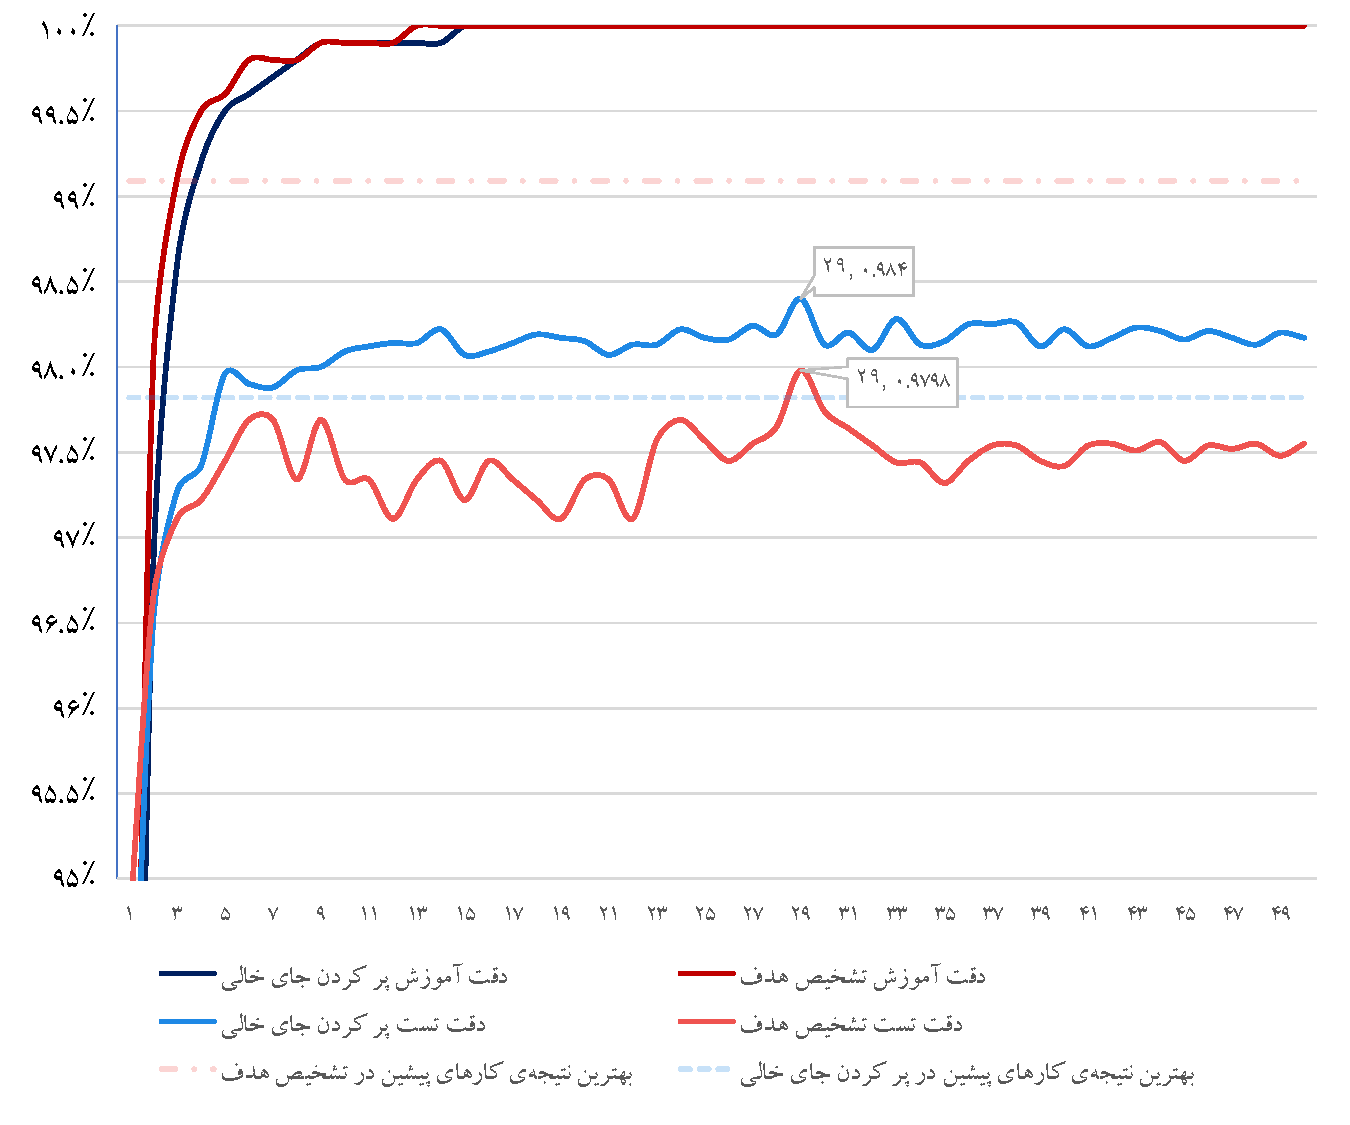
\includegraphics[scale=0.65]{Figures/atis_training_journey.pdf}
	\caption{شیب آموزش مدل پیشنهادی بر روی مجموعه داده‌ی \lr{ATIS}.}
	\label{Fig:atis_journey}
\end{figure}
شکل \ref{Fig:atis_journey} شیب آموزش مدل پیشنهادی به همراه $BERT_{large}$ را بر روی مجموعه داده‌ی \lr{ATIS} نشان می‌دهد. در راستای تحلیل وظیفه‌ی پر کردن جای خالی، در طول شیب آموزش مشاهده می‌شود که مدل در بازه‌ی دور ۱ تا ۱۰، دارای یک حداکثر محلی است. مدل در همین بازه نیز از کارهای پیشین سبقت می‌گیرد. برخی از کار‌های پیشین محدودیت ۱۰ دور را بر روی آموزش مدل اعمال کردند. در طول آزمایش‌ها مشاهده شد که مدل پس از اینکه در طول ۱۰ دور اول، مدل به حداکثر محلی رسیده و سپس رشد آن متوقف شده و گاهی کاهش می‌یابد. در این بازه، مدل شروع به حداکثر برازش خود رسیده و دقت مدل روی مجموعه‌ی آموزشی، به ۱۰۰درصد رسیده است. محدودیت تعداد دور آموزشی روی ۵۰ دور تنظیم شد. از این رو، پس از ۱۰ دور آموزش، مشاهده می‌شود که دقت مدل ثابت بوده و گاهی کاهش می‌یابد؛ اما در ادامه و در دور ۲۹-ام، حداکثر سراسری اتفاق می‌افتد و بیشترین دقت مدل کسب می‌شود. امتیاز مدل در وظیفه‌ی پر کردن جای خالی، پس از دور ۲۹-ام نیز به طور متوسط از دور ۱۰ تا ۲۹ بیشتر است. این پدیده، در \cite{doubledescent} نیز مورد بررسی قرار گرفته و نام آن را فرود عمیق دوگانه\LTRfootnote{Deep Double Descent} گذاشتند. فرود عمیق دوگانه بیان می‌کند که با بزرگ شدن اندازه‌ی مدل، دقت مدل بر روی داده‌ی آموزشی، ابتدا کاهش و سپس افزایش پیدا می‌کند. این قضیه برای تعداد دورهای آموزشی وجود دارد؛ جایی که مدل ابتدا به یک قله‌ی محلی می‌رسد، سپس دچار سکون یا افت دقت می‌شود، و سپس با ادامه دادن فرایند آموزش، دقت آن به تدریج زیادتر می‌شود و عملکرد بهتری از قله‌ی اولیه نشان می‌دهد \cite{doubledescent}. این قضیه، به وضوح در وظیفه‌ی تشخیص هدف در شکل \ref{Fig:atis_journey} مشهود است؛ جایی که مدل بعد از دور ۱۰-ام آموزش، تا دور ۲۴-ام دچار افت شدید دقت شده، و سپس در دور ۲۹-ام حداکثر دقت را نمایش می‌دهد. همچنین، بعد از این قله، میانگین دقت مدل، از پیش از قله بیشتر است.
\begin{figure}[!htb]
	\centering
	\includegraphics[scale=0.65]{Figures/snips_training_journey.pdf}
	\caption{شیب آموزش مدل پیشنهادی بر روی مجموعه داده‌ی \lr{SNIPS}.}
	\label{Fig:snips_journey}
\end{figure}
شکل \ref{Fig:snips_journey} شیب آموزش مدل پیشنهادی، بر روی مجموعه داده‌ی \lr{SNIPS} را به همراه $BERT_{large}$ ترسیم می‌کند. به نظر می‌رسد اندازه‌ی بزرگتر مجموعه داده‌ی \lr{SNIPS}، باعث کمتر شدن اثر افت دقت در طول فرایند آموزش شده است. آنطور که در شکل \ref{Fig:snips_journey} مشهود است، مدل در ۱۰ دور ابتدایی آموزش، برای هر دو وظیفه، دچار نوسان بوده و بلافاصله بعد از دور ۱۰-ام دچار افت شدید دقت شد. همچنین، دقت مدل در مجموعه‌ی آموزشی، در دور ۱۰-ام به ۱۰۰درصد رسیده است. در چنین شرایطی، مدلی که از مکانیزم توقف زودرس استفاده کند، آموزش را متوقف کرده و دچار حداکثر دقت محلی می‌شود. در همین راستا، مدل‌هایی مانند \cite{e:2019,goo-etal-2018-slot} که محدودیت ۱۰ دور را بر روی دور آموزش اعمال کردند، دچار این مسئله هستند. مدل پیشنهادی بعد از دور ۱۳-ام مجددا دچار افزایش دقت شد و در دور ۲۹ و ۳۰ بهترین عملکرد را از خود نمایش داد. علاوه بر این، میانگین دقت مدل بعد از قله، بیشتر از قبل قله است. دقت مدل پیشنهادی بر روی وظیفه‌ی پر کردن جای خالی، از دور ۴-ام از بیشترین دقت کارهای قبلی، پیشی می‌گیرد که این بیانگر توانایی تعمیم مدل پیشنهادی است.
\section{خطاهای باقی مانده}
همانطور که در جدول نتایج مشخص است، دقت مدل‌های پیشنهادی بسیار بالا و نزدیک به ۱۰۰ درصد است. مدل پیشنهادی در این پایان‌نامه، بالاترین دقت را در وظیفه‌ی پر کردن جای خالی به دست آورد. با توجه به این که تعداد نمونه‌های موجود در مجموعه‌ی تست، که مدل قادر به پیش‌بینی صحیح آن نیست، کم است، بهتر است برای ارائه یک مدل بهتر، ضعف‌های موجود در مدل را شناخته شود و با آگاهی نسبت به آن‌ها، معماری جدید پیشنهاد شود. از این جهت، در پیوست پایان‌نامه، تمام خطاهایی که برای وظیفه‌ی تشخیص هدف رخ داده، فهرست شده‌اند. همچنین، در بخش پیش رو، نمونه‌هایی را که مدل اشتباه پیش‌بینی می کند، تحلیل می‌شوند.
\subsection{تحلیل خطاها‌ی مدل پیشنهادی در \lr{ATIS}}
در مجموعه داده‌ی \lr{ATIS}، ۱۸ خطا در وظیفه‌ی تشخیص هدف، توسط مدل پیشنهادی رخ داد. ۵ مورد از این خطاها شامل مواردی است که برچسب هدف در زمان آموزش دیده نشد است. این برچسب‌ها، \lr{atis\_airfare\#atis\_flight}، \lr{atis\_day\_name}، \lr{atis\_flight\#atis\_airline} و \lr{atis\_flight\_no\#atis\_airline} هستند. با توجه به ماهیت چالش درک زبان طبیعی، نباید در طراحی معماری، از تجزیه‌گر برچسب، یا واژه‌های توصیفی برای برچسب‌ها و اهداف استفاده شود. از این رو، در زمان تست هرگز امکان حدس صحیح این اهداف، یا تشخیص آن‌ها از یکدیگر، وجود ندارد. همچنین، تعداد زیادی از خطاها به خاطر حدس یک برچسب برای هدف‌هایی است که ترکیبی هستند. در چنین شرایطی، مدل پیشنهادی تنها برچسب هدف اول را پیش‌بینی می‌کند و در پیش‌بینی برچسب ترکیبی ضعف دارد. با مشاهده‌ی لیست خطاها، مشهود است که در مجموعه داده‌ی \lr{ATIS}، با وجود حدس صحیح و کامل برچسب‌ها، هدف نهائی اشتباه حدس زده شده است. این موضوع، ممکن است بخاطر ادغام ضعیف دو وظیفه‌ی تشخیص هدف و پر کردن جای خالی، در مدل پیشنهادی باشد. در برخی از خطاها، مشاهده می‌شود که مدل، اشتباهاتی را به علت ابهام در مثال‌های آموزشی می‌دهد. به طور مثال، با مشاهده‌ی جمله‌ی \lr{"how many northwest flights leave st. paul"}، مدل، هدف \lr{atis\_quantity} را پیش‌بینی می‌کند. با بررسی دقیق‌تر نمونه‌های آموزشی مشاهده می‌شود که این تصمیم،  با نمونه‌هایی مانند \lr{"how many united flights are there from san francisco please"} که دارای مقدار تشخیص هدف \lr{atis\_quantity} است، همخوانی دارد؛ از این رو، نمی‌توان این نوع خطا ها را متوجه معماری دانست.
\subsection{تحلیل خطاهای مدل پیشنهادی در \lr{SNIPS}}
مدل پیشنهادی ما، در مجموعه داده‌ی \lr{SNIPS}، ۴ تشخیص اشتباه در وظیفه‌ی تشخیص هدف دارد. چیزی که میان خطاهای مذکور مشترک است، طول کوتاه آن‌ها است. در مجموعه داده‌ی \lr{SNIPS}، میانگین طول جمله برابر ۹ است و در خطاهای موجود، میانگین طول برابر ۵‍.‍۲۵ است. همچنین، مجدداً در خطاها مشاهده می‌شود که با وجود تشخیص صحیح تمام برچسب‌ها، هدف پیش‌بینی شده با هدف صحیح تفاوت دارد.
\chapter{نتیجه‌گیری}
\pagebreak
در این پایان‌نامه، \lr{CTran}، که مدلی مبتنی بر شبکه‌ی کانولوشنی و ترنسفورمر است، برای درک زبان طبیعی ارائه شد. مدل پیشنهادی از معماری رمزنگار-رمزگشا بهره می‌برد و برای آموزش دو وظیفه‌ی تشخیص هدف و پر کردن جای خالی، از یک رمزنگار اشتراکی استفاده می‌کرد. در معماری پیشنهادی، مدل زبانی برت به عنوان تعبیه‌گر واژه‌ها استفاده شد. سپس نمایش جدیدی از کلمات با استفاده از شبکه‌ی کانولوشنی ایجاد و به جای عملیات \lr{Pooling}، از ساختار توالی ویژگی پنجره استفاده شد. برای حفظ رابطه‌ی یک به یک واژه‌های ورودی با برچسب‌های هدف، اندازه هسته‌ی ۱ در شبکه‌ی کانولوشنی در کنار سایر اندازه‌ها هسته اضافه شد. همچنین برای ادغام معنای واژه‌های همسایه در یکدیگر، اندازه هسته‌های ۱ تا ۵، به صورت ترکیبی استفاده شد. در نهایت، از پشته‌ی رمزنگار ترنسفورمر برای ایجاد تعبیه‌ی نهائی واژه‌ها بهره برده شد. در معماری \lr{CTran} برای هر وظیفه، یک رمزگشا تعریف شد.
برای وظیفه‌ی تشخیص هدف، از توجه به خود و به دنبال آن یک لایه کاملاً متصل استفاده گردید.  همچنین، رمزگشای ترنسفورمر تراز شده برای وظیفه‌ی پر کردن جای خالی معرفی و ضمن ساخت یک پشته از آن، برچسب‌های هدف تولید شدند.  در پایان، مدل پیشنهادی با مدل‌های شناخته‌شده مقایسه شد و نتایج نشان داد که مدل \lr{CTran} در وظیفه‌ی پر کردن جای خالی از مدل‌های موجود بهتر عمل می‌کند. 


در این پایان‌نامه، دو سیاست مدل زبانی به جای رمزنگار و مدل زبانی به عنوان تعبیه برای به کارگیری مدل‌های زبانی در معماری شبکه آزمایش شد و نتایج نشان داد که استفاده از مدل‌های زبانی به عنوان تعبیه‌ی کلمه، استراتژی بهتری نسبت به ترکیب آن‌ها در ساختار شبکه دارد. در مقابل، استفاده از مدل‌های زبانی به عنوان تعبیه، به معنای معرفی یک رمزنگار جدا برای شبکه و در نتیجه، معرفی پارامترهای جدید به شبکه است. این امر ذاتاً باعث ایجاد بار محاسباتی جدید می‌شود. از این رو،  تاثیر این دو استراتژی در سرعت آموزش و سرعت استنتاج، اندازی گیری شد و تاخیر اضافه‌ی ایجاد شده در شبکه گزارش گردید.


در پایان کار، مواردی هست که می‌توان در آینده آن‌ها را بررسی کرد.\\
\textbf {\ding{118}معرفی یک مکانیزم برای تزریق صریح هدف به وظیفه‌ی پر کردن جای خالی یا برعکس:} 
در این شیوه، با تزریق بردار تعبیه‌ی اهداف یا بردار توجه آن‌ها، به رمزگشای پر کردن جای خالی، مدل را به منظور انتخاب برچسب‌های صحیح راهنمایی می‌کنند. ما در این راستا، دو سیاست را برای ترکیب خروجی‌ها آزمایش کردیم؛ سیاست اول، میانگین‌گیری از ماتریس تفکر برچسب، تبدیل آن به بردار و ترکیب آن با بردار توجه تشخیص هدف، بود. سیاست دوم، الحاق خروجی تشخیص هدف با هر برچسب، قبل از لایه‌ی خطی که ابعاد آن را کاهش می‌دهد، بود. ما هیچ بهبودی پس از اعمال این دو سیاست در مدل مشاهده نکردیم؛ از این رو نتایج آن در این پایان نامه ذکر نشده است. تحقیقات آینده می‌تواند به معرفی مکانیزمی برای ترکیب بهینه‌ی این دو وظیفه با یکدیگر بپردازد.\\
\textbf {\ding{118}مدل زبانی مبتنی بر شبکه‌ی کانولوشنی و ترنسفورمر:}
در این پژوهش، مشاهده شد که استفاده از شبکه‌ی کانولوشنی با پشته‌ی رمزنگار ترنسفورمر عملکرد شبکه را بهبود می‌بخشد. این نتیجه، نوید از سودمندی این معماری می‌دهد؛ بنابراین در آینده می‌توان یک مدل زبانی مبتنی بر کانولوشن-ترنسفورمر معرفی کرد و عملکرد آن را با مدل زبانی برت سنجید.\\
\textbf {\ding{118}آزمایش معماری در سایر وظیفه‌ها:} 
همان‌طور که در فصل اول گفته شد، معماری معرفی شده برای درک زبان طبیعی، کاربرد گسترده‌ای در پردازش زبان طبیعی دارد؛ چرا که خروجی آن به شکلی است که امکان استفاده از این ساختار شبکه را در بسیاری از وظایف پردازش زبان طبیعی می‌دهد. در پژوهش‌های آینده، می‌توان عملکرد این معماری در سایر وظایف را نیز سنجید. این سنجش نیازی به تغییر ساختار معماری ندارد و مدل عیناً قابلیت جابجایی برای وظایف یاد شده در فصل اول را دارد. همچنین، با بسط دادن معماری، می توان آن را در سایر وظایفی که نامی از آن‌ها برده نشده است نیز به کار گرفت.\\
\textbf {\ding{118}بررسی دقیق‌تر مدل‌های زبانی:} 
ما در پژوهش خود، عملکرد دو مدل زبانی المو و برت را سنجیدیم. ما همچنین عملکرد مدل را با سایر مدل‌های زبانی مطرح که شامل اکس ال نت\LTRfootnote{XLNet}، روبرت\LTRfootnote{RoBert}، الکترا\LTRfootnote{Electra} هستند نیز سنجیدیم. عملکرد این مدل‌ها در مقابل برت بر روی معماری ما بهبودی نداشت؛ اما از طرفی مقایسه‌ی انجام شده عادلانه نبود. علت ناعادلانه بودن آن، آموزش برت بر روی داده‌هایی با حروف کوچک بود؛\LTRfootnote{Uncased}. متن جملات در هر دو مجموعه داده‌ی \lr{ATIS}‌ و \lr{SNIPS}، با حروف کوچک است. این درحالی است که مدل‌های زبانی روبرت، الکترا و اکس ال نت، بر روی مجموعه داده‌ی با حروف کوچک و بزرگ\LTRfootnote{Cased} آموزش داده شده‌اند. از این رو، در جدول نتایج این پایان نامه، نتایج مربوط به سه مدل زبانی یاد شده، درج نشده است. در آینده می‌توان به دو روش، مقایسه‌ی عادلانه‌ای، بین این مدل‌های زبانی برای وظیفه‌ی درک زبان طبیعی انجام داد. نخست، آموزش مدل‌های زبانی مذکور بر روی داده‌های حروف کوچک است که این مورد از نظر هزینه‌ی محاسباتی، بار سنگینی دارد. دوم، تغییر جملات مجموعه داده به حروف کوچک و بزرگ است که نیازمند نیروی کار و هزینه‌ی مادی است.

% ░░░░░░░▒▒▒▒▒▒▓▓▓▓ Appendices ▓▓▓▓▒▒▒▒▒▒░░░░░░░
\MakeAppendices
\section{جزئیات اشتباهات مدل}
\setlength{\hoffset}{0cm}
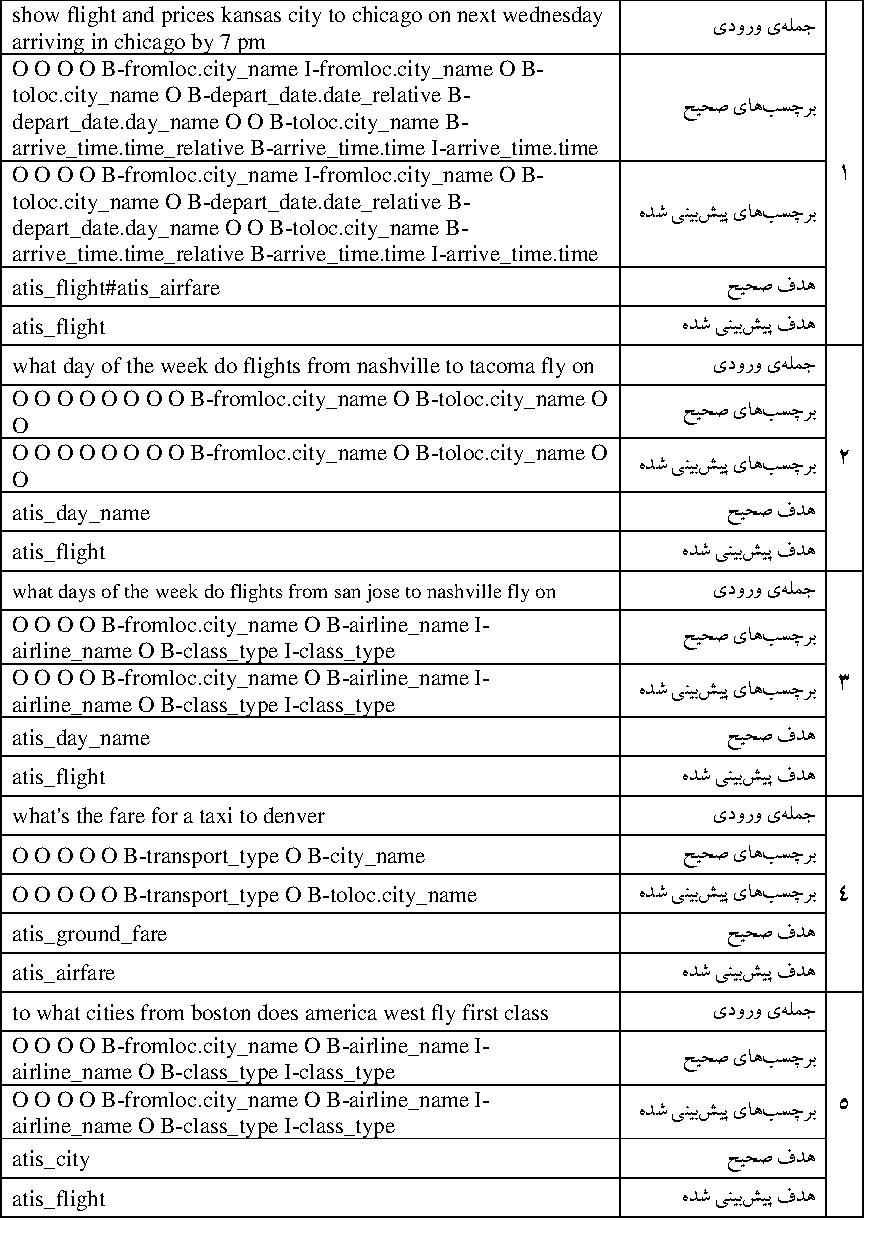
\includepdf[pages=1,nup=1x1,pagecommand={\rl{\subsection{اشتباهات در مجموعه داده‌ی\lr{ATIS}}}}\vspace{-\baselineskip},width=(\textwidth*8/9)]{Tables/atiserrors.pdf}
\includepdf[pages=2-,nup=1x1,pagecommand={},width=(\textwidth*1)]{Tables/atiserrors.pdf}
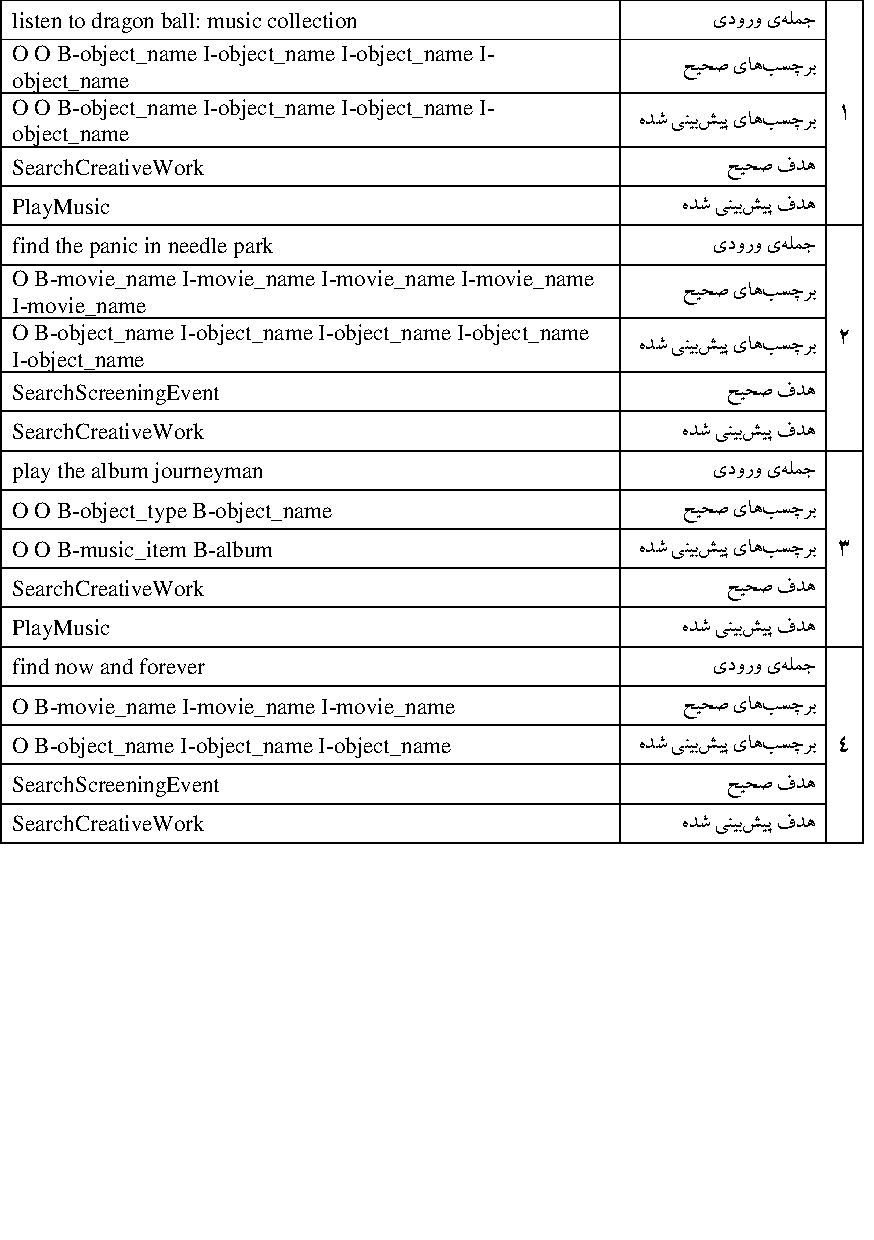
\includepdf[pages=1,nup=1x1,pagecommand={\rl{\subsection{اشتباهات در مجموعه داده‌ی\lr{SNIPS}}}}\vspace{-\baselineskip},width=(\textwidth*8/9)]{Tables/snipserrors.pdf}
%\includepdf[pages=2-,nup=1x1,pagecommand={},width=(\textwidth*1)]{Tables/snipserrors.pdf}


% ░░░░░░░▒▒▒▒▒▒▓▓▓▓ References ▓▓▓▓▒▒▒▒▒▒░░░░░░░
\MakeReferences
%\bibliographystyle{Settings/ModifiedIEEEtranFa}
%\bibliographystyle{ieeetr}
\bibliographystyle{Settings/IEEEtran}
%\lr{\bibliography{References}}
\bibliography{References}
% ░░░░░░░▒▒▒▒▒▒▓▓▓▓ ENtoFA Vocabulary ▓▓▓▓▒▒▒▒▒▒░░░░░░░
\MakeEnVocab
% ░░░░░░░▒▒▒▒▒▒▓▓▓▓ FAtoEN Vocabulary ▓▓▓▓▒▒▒▒▒▒░░░░░░░
\MakeFaVocab

% ░░░░░░░▒▒▒▒▒▒▓▓▓▓ Abstract - English ▓▓▓▓▒▒▒▒▒▒░░░░░░░
\DepartmentEn{Department of Electrical and Computer Engineering}
%%\DegreeEn{Doctor of Philosophy (PhD)} % Or 
\DegreeEn{Master of Science (MSc)} 
\YourFullnameEn{Mehrdad RafiePour}
\YourEmailAddress{rafiepour@grad.kashanu.ac.ir}
\DateEn{19/2/2023}
\FirstSupervisorEn{Javad Salimi Sartakhti, Prof.}
\FirstSupervisorEmailAddress{salimi@kashanu.ac.ir}
\FirstAdvisorEn{Fereshteh Dehghani, Prof.}
\FirstAdvisorEmailAddress{fdehghani@kashanu.ac.ir}
%\SecondSupervisorEn{Fereshteh Dehghani, Prof.} % Optional (Remove It If You Don't Have)
%\SecondSupervisorEmailAddress{dehghani@kashanu.ac.ir} % Optional (Remove It If You Don't Have)
\TitleEn{Proposing a Model for Natural Language Understanding  \\[0.2cm] Using Deep Neural Networks}
% اگر عنوان رساله طولانی بود، در دو خط به صورت نشان داده شده تقسیم شود.

\AbstractEn{
	With the increasing popularity of smartphones, adoption of dialogue-system-based tools have seen significant growth.  Natural language understanding is a key component of dialogue systems, as it can be a major bottleneck in the dialogue system workflow. Intent-detection and slot-filling are the two main tasks in natural language understanding. Recurrent Neural Networks have been extensively explored to improve these tasks, but they have well-established weaknesses, namely gradient vanishing and high training time. Recently, Transformer was introduced to rectify said flaws. Moreover, we observed that only a few models further encode the pre-trained language model's output. In this thesis, CTran is propose. CTran is a novel encoder-decoder CNN-Transformer-based architecture designed for intent-detection and slot-filling. In the encoder, BERT is utilized as a word embedding. Then, several convolutional layers with different kernel sizes are used, which are then transposed and concatenated. In the last part of the encoder, stacked Transformer encoders are used to provide final output of the encoder. For the intent-detection decoder, self-attention is utilized followed by a linear layer. In the slot-filling decoder, the aligned Transformer decoder is introduced, which utilizes a heuristical diagonal mask. The diagonal mask provides access to encoder positions which correspond to each target token, and hides other positions. Finally, to evaluate the performance of the proposed model, it is applied on ATIS and SNIPS. The results show that CTran achieve better results than the current state-of-the-art in slot-filling on both datasets.  Furthermore, two strategies, meaning language model as word embedding, and language model as an encoder, are compared. The results show that language model as word embedding strategy yields a better result.
}

\KeywordsEn{1-Deep Neural Networks, 2-Natural Language Processing, 3- Natural Language Understanding, 4-Intent-Detection, 5-Slot-Filling}
\MakeEnglishAbstract

% ░░░░░░░▒▒▒▒▒▒▓▓▓▓ Signature - English ▓▓▓▓▒▒▒▒▒▒░░░░░░░
\FirstAdvisorEn{Fereshteh Dehghani, Prof.}
%\SecondAdvisorEn{Second Advisor, Assist. Prof.} % Optional (Remove It If You Don't Have)
\FirstExaminerEn{First Examiner, Prof.}
\SecondExaminerEn{Second Examiner, Prof.} % Optional (Remove It If You Don't Have)
%\ThirdExaminerEn{Third Examiner, Prof.} % Optional (Remove It If You Don't Have)
%\FourthExaminerEn{Fourth Examiner, Prof.} % Optional (Remove It If You Don't Have)
%\FifthExaminerEn{Fifth Examiner, Prof.} % Optional (Remove It If You Don't Have)
\DeanOfDepartmentEn{Dean, Prof.}

%\MakeEnglishSignaturePage

\end{document} 
